\documentclass[a4paper, nofonts, notoc]{tufte-book}

	\title{Stata for Social Scientists}
	\author{François Briatte}
	\publisher{\url{http://f.briatte.org/teaching/quanti/}}

	\usepackage[utf8]{inputenc}

%
% fonts
%
\usepackage{libertine}
\usepackage{inconsolata}

%
% math
%
\usepackage{amsmath}
\usepackage{amssymb}

%% maxwidth is the original width if it is less than linewidth
%% otherwise use linewidth (to make sure the graphics do not exceed the margin)
\makeatletter
\def\maxwidth{ %
  \ifdim\Gin@nat@width>\linewidth
    \linewidth
  \else
    \Gin@nat@width
  \fi
}
\makeatother
\usepackage{framed}
\makeatletter
\newenvironment{kframe}{%
 \def\at@end@of@kframe{}%
 \ifinner\ifhmode%
  \def\at@end@of@kframe{\end{minipage}}%
  \begin{minipage}{\columnwidth}%
 \fi\fi%
 \def\FrameCommand##1{\hskip\@totalleftmargin \hskip-\fboxsep
 \colorbox{shadecolor}{##1}\hskip-\fboxsep
     % There is no \\@totalrightmargin, so:
     \hskip-\linewidth \hskip-\@totalleftmargin \hskip\columnwidth}%
 \MakeFramed {\advance\hsize-\width
   \@totalleftmargin\z@ \linewidth\hsize
   \@setminipage}}%
 {\par\unskip\endMakeFramed%
 \at@end@of@kframe}
\makeatother

\definecolor{fgcolor}{rgb}{0.2, 0.2, 0.2}
\definecolor{shadecolor}{rgb}{.97, .97, .97}
\definecolor{messagecolor}{rgb}{0, 0, 0}
\definecolor{warningcolor}{rgb}{1, 0, 1}
\definecolor{errorcolor}{rgb}{1, 0, 0}
\newenvironment{knitrout}{}{} % an empty environment to be redefined in TeX

%
% table of contents
%
\usepackage{minitoc}
	\dominitoc[n]
	\nomtcrule
	\setcounter{secnumdepth}{1}

%
% tables
%
\usepackage{booktabs}

%
% cover image
%
\usepackage{tabularx}

%
% diagrams
%
\usepackage{tikz}
\usepackage{circuitikz}
	%
	% ColorBrewer Set1 for \tikz figures, by Timothée Poisot
	% See: http://timotheepoisot.fr/2012/07/03/colorbrewer-in-pgfplots/
	%
	\definecolor{s1}{RGB}{228, 26, 28}
	\definecolor{s2}{RGB}{55, 126, 184}
	\definecolor{s3}{RGB}{77, 175, 74}
	\definecolor{s4}{RGB}{152, 78, 163}
	\definecolor{s5}{RGB}{255, 127, 0}

%
% images
%
\usepackage{graphicx}
	\setkeys{Gin}{width=\linewidth,totalheight=\textheight,keepaspectratio}
	\graphicspath{{images/}}

%
% links
%
\hypersetup{colorlinks}

%
% verbatims
%
\usepackage{fancyvrb}
	\fvset{fontsize=\normalsize}

%%
% Prints argument within hanging parentheses (i.e., parentheses that take
% up no horizontal space).  Useful in tabular environments.
\newcommand{\hangp}[1]{\makebox[0pt][r]{(}#1\makebox[0pt][l]{)}}

%%
% Prints an asterisk that takes up no horizontal space.
% Useful in tabular environments.
\newcommand{\hangstar}{\makebox[0pt][l]{*}}

%
% trailing spaces
%
\usepackage{xspace}

%
% month-year
%
\newcommand{\monthyear}{%
  \ifcase\month\or January\or February\or March\or April\or May\or June\or
  July\or August\or September\or October\or November\or
  December\fi\space\number\year
}

%
% citations
%
\newcommand{\footcite}[1]{\citeauthor{#1}\cite{#1}}

%
% blank page
%
\newcommand{\blankpage}{\newpage\hbox{}\thispagestyle{empty}\newpage}
 % style
	%%% DATASETS

\newcommand{\ess}{European Social Survey\xspace}
\newcommand{\ESS}{\textsc{ess}\xspace}

\newcommand{\gss}{General Social Survey\xspace}
\newcommand{\GSS}{\textsc{gss}\xspace}

\newcommand{\nhis}{National Health Interview Survey\xspace}
\newcommand{\NHIS}{\textsc{nhis}\xspace}

\newcommand{\qog}{Quality of Government\xspace}
\newcommand{\QOG}{\textsc{qog}\xspace}

\newcommand{\wvs}{World Values Survey\xspace}
\newcommand{\WVS}{\textsc{wvs}\xspace}

%%% HANDLES

\newcommand{\SSC}{\textsc{ssc}\xspace}
\newcommand{\PDF}{\textsc{pdf}\xspace}
\newcommand{\URL}{\textsc{url}\xspace}
\newcommand{\ZIP}{\textsc{zip}\xspace}
\newcommand{\SRQM}{\textsc{srqm}\xspace}
\newcommand{\README}{\texttt{README}\xspace}

\newcommand{\TL}{Tufte-\LaTeX\xspace}

%%% FOLDERS

\newcommand{\course}{\texttt{course}\xspace}
\newcommand{\data}{\texttt{data}\xspace}
\newcommand{\setup}{\texttt{setup}\xspace}
\newcommand{\code}{\texttt{code}\xspace}
 % word shortcuts
	\newcommand{\hlred}[1]{\textcolor{Maroon}{#1}} % prints in red

\newcommand{\kbd}[1]{\texttt{#1}\index{Keyboard shortcuts!#1}} % index keyboard shortcuts; TODO: differentiate Mac and PC
\newcommand{\ext}[1]{\texttt{#1}\index{File extensions!#1}} % index file extensions
\newcommand{\statacode}[1]{\texttt{#1}}
\newcommand{\filename}[1]{\texttt{#1}}

%%
%% Indexing of Stata commands.
%%

% \newcommand{\application}[1]{{\sffamily\subsection{#1}}}

% index for Stata commands: \cmd[shorthand]{command}
% ------------------------
\newcommand{\cmd}[2][]{%
	\ifthenelse{\isempty{#1}}%
		{% index command
			\hlred{\texttt{#2}}%
			\index{#2 command@\protect\texttt{#2}}% command name
		}%
		{% index command and shorthand
			\hlred{\texttt{#2}} (\hlred{\texttt{#1}})%
			\index{#2 command@\protect\texttt{#2} (shorthand: \texttt{#1})}%
		}%
}

% index for Stata command options: \opt or \coab for abbreviations
% -----------------------
\newcommand{\opt}[2]{\hlred{\texttt{#1}}\index{#1@\texttt{#1} (option to \texttt{#2})}\xspace}
\newcommand{\coab}[3]{\hlred{\texttt{#1}} (\hlred{\texttt{#2}})\index{#1@\texttt{#1} (\texttt{#2}; option to \texttt{#3})}\xspace}

% index for Stata packages: \pkg{package} (on first instance of external command)
% -----------------------
\newcommand{\pkgfirst}[1]{%
	\footnote{Requires the \cmd{#1} package, which installs from the online \SSC archive with the following command:\\\statacode{ssc install #1}}%
	\index{#1 command@\protect\texttt{#1}!installation@\protect installation of the \texttt{#1} package}% command name
}
\newcommand{\pkg}[1]{\texttt{#1}\index{#1 package@\protect\texttt{#1} package}\index{Packages!#1@\texttt{#1}}}% package name

% Macros for typesetting the documentation

%
% used for Stata code environments:
%
\newenvironment{docspec}{\begin{quotation}\ttfamily\parskip0pt\parindent0pt\ignorespaces}{\end{quotation}}% command specification environment

%
% \TL unused:
%

\newcommand{\hangleft}[1]{\makebox[0pt][r]{#1}}
\newcommand{\hairsp}{\hspace{1pt}}% hair space
\newcommand{\hquad}{\hskip0.5em\relax}% half quad space
\newcommand{\TODO}{\textcolor{red}{\bf TODO!}\xspace}
\newcommand{\ie}{\textit{i.\hairsp{}e.}\xspace}
\newcommand{\eg}{\textit{e.\hairsp{}g.}\xspace}
\newcommand{\na}{\quad--}% used in tables for N/A cells

\providecommand{\XeLaTeX}{X\lower.5ex\hbox{\kern-0.15em\reflectbox{E}}\kern-0.1em\LaTeX}
\newcommand{\tXeLaTeX}{\XeLaTeX\index{XeLaTeX@\protect\XeLaTeX}}

% \index{\texttt{\textbackslash xyz}@\hangleft{\texttt{\textbackslash}}\texttt{xyz}}
\newcommand{\doccmdnoindex}[2][]{\texttt{#2}}% command name -- adds backslash automatically (and doesn't add cmd to the index)

\newcommand{\doccmddef}[2][]{%
  \hlred{\texttt{#2}}\label{cmd:#2}%
  \ifthenelse{\isempty{#1}}%
    {% add the command to the index
      \index{#2 command@\protect\texttt{#2}}% command name
    }%
    {% add the command and package to the index
      \index{#2 command@\protect\texttt{#2} (\texttt{#1} package)}% command name
      \index{#1 package@\texttt{#1} package}\index{packages!#1@\texttt{#1}}% package name
    }%
}% command name -- adds backslash automatically

\newcommand{\doccmd}[2][]{%
  \texttt{#2}%
  \ifthenelse{\isempty{#1}}%
    {% add the command to the index
      \index{#2 command@\protect\texttt{#2}}% command name
    }%
    {% add the command and package to the index
      \index{#2 command@\protect\texttt{#2} (\texttt{#1} package)}% command name
      \index{#1 package@\texttt{#1} package}\index{packages!#1@\texttt{#1}}% package name
    }%
}% command name -- adds backslash automatically
\newcommand{\docopt}[1]{\ensuremath{\langle}\textrm{\textit{#1}}\ensuremath{\rangle}}% optional command argument
\newcommand{\docarg}[1]{\textrm{\textit{#1}}}% (required) command argument

% \newcommand{\docenv}[1]{\texttt{#1}\index{#1 environment@\texttt{#1} environment}\index{environments!#1@\texttt{#1}}}% environment name
% \newcommand{\docenvdef}[1]{\hlred{\texttt{#1}}\label{env:#1}\index{#1 environment@\texttt{#1} environment}\index{environments!#1@\texttt{#1}}}% environment name
% \newcommand{\doccls}[1]{\texttt{#1}}% document class name
% \newcommand{\docclsopt}[1]{\texttt{#1}\index{#1 class option@\texttt{#1} class option}\index{class options!#1@\texttt{#1}}}% document class option name
% \newcommand{\docclsoptdef}[1]{\hlred{\texttt{#1}}\label{clsopt:#1}\index{#1 class option@\texttt{#1} class option}\index{class options!#1@\texttt{#1}}}% document class option name defined
% \newcommand{\docmsg}[2]{\bigskip\begin{fullwidth}\noindent\ttfamily#1\end{fullwidth}\medskip\par\noindent#2}


% \newcommand{\docmsg}[2]{%\medskip
%   \noindent\texttt{#1}%\medskip
%   \par\noindent#2\bigskip}

% \newcommand{\docfilehook}[2]{\texttt{#1}\index{file hooks!#2}\index{#1@\texttt{#1}}}
% \newcommand{\doccounter}[1]{\texttt{#1}\index{#1 counter@\texttt{#1} counter}}

% Generates the index
\usepackage{makeidx}
\makeindex

 % documentation index

\begin{document}

% Front matter
\frontmatter

  %
% r-1
%
\newpage

\begin{fullwidth}
	
	\thispagestyle{empty}
	\setlength{\parindent}{0pt}
	\setlength{\parskip}{\baselineskip}

	\vskip 8em

	{
		\LARGE%
		\par%
			\smallcaps{François Briatte}%
			%
	}\\[0.167\textheight]

	\vfill
		
	\makebox[\textwidth]{%
		\begin{tabularx}{1.5\textwidth}{XX}
		  
\includegraphics[width=\paperwidth]{0-this-is-stata}
		\end{tabularx}}
		
	\vfill

	\par%
		\textit{This is release \texttt{0.988} from \monthyear.}
	
\end{fullwidth}

\cleardoublepage
 %% r-1
  %
% r-3
%
\newpage

\begin{fullwidth}

	\thispagestyle{empty}
	\setlength{\parindent}{0pt}
	\setlength{\parskip}{\baselineskip}

	\vskip 8em

	{
		\LARGE%
		\par%
			\smallcaps{François Briatte}%
			%
	}\\[0.167\textheight]
		
	\vfill
		
	{\normalsize\smallcaps{this is stata, or}}\\[.5\baselineskip]
	{\huge\allcaps{Stata for social scientists}}\\[\baselineskip]

	\vfill

	\index{Acknowledgements}%
	%
  \smallcaps{Acknowledgements} go first and foremost to Ivaylo Petev, with whom I co-taught many of the classes for which this guide was written, and to the students who offered their invaluable feedback on earlier draft versions, with a special mention to Laura Führer. I have also benefitted from the friendly advice of Baptiste Coulmont, Emiliano Grossman, Filip Kostelka, Sarah McLaughlin, Dawn Teele, Vincent Tiberj and Hyungsoo Woo. Final thanks to the \textsc{psia} and \textsc{glm} staff at Sciences Po for their excellent support. All mistakes are mine alone.%

	\par%
		\textit{Please do not cite this draft and send all feedback to %
		\href{mailto:f.briatte@ed.ac.uk}{f.briatte@ed.ac.uk}.}

\end{fullwidth}

\cleardoublepage
 %% r-3

	\newpage%
  \tableofcontents %% r-5
	\cleardoublepage
	
\mainmatter %% r-7

  %
% 1
%
\chapter{Introduction}%
	%
	\label{ch:intro}
	\index{Course!Introduction}%
	%
  \begin{mybox}%
    %
    \newthought{Dear reader,}\\[1em]%
  	%
  	You probably find yourself reading this because you enrolled in Statistical Reasoning and Quantitative Methods (\SRQM), a postgraduate introduction to statistics that Ivaylo Petev and myself have been teaching at Sciences~Po in Paris since 2010.\\[1em]%
    %
    Welcome to the course.\\[1em]%
    %
    \smallcaps{This guide} is a practical handbook to read while taking the course. The rest of the teaching material, which includes the syllabus and essential files to be used in and outside class, can be downloaded from the course webpage at the following address:\\[1em]%
      %
      \url{http://f.briatte.org/teaching/quanti/}\\[1em]%
      %
  	%
    \smallcaps{Start reading below} to learn about the course basics, making sure in particular that you have \textbf{run the course setup} on your computer and that you know how to run it again if necessary. Welcome again, and see you soon.%
    %  
  \end{mybox}\\[4em]%
  %
  \startcontents[chapters]%
  \printcontents[chapters]{l}{1}{\setcounter{tocdepth}{2}}%
	%
	\newpage%
	%

%
% 1.1 course topics
%
%
% 1.1
%
% \section{Topics}%
%   %
%   %
%   \label{sec:topic}%
	\index{Methods}%
	%
	%

% 1.1.1
%
% \subsection{Quantitative methods}
%   %
%   %
	\label{sec:quantitative-methods}
  \index{Quantitative methods}%
  
	\newthought{Quantitative methods} designate a branch of social science methodology that applies statistical procedures to experimental or observational data in order to produce explanatory models for the complex, recurrent phenomena that affect populations and organizations. These methods can be used to analyze things like attitudes towards highly skilled and low-skilled immigration in the United States,\footcite{HainmuellerHiscox:2010a} the effects of a program to develop fertilizer use in Kenya,\footcite{DufloKremer:2009a} or the historical vote that put Adolf Hitler into power in interwar Germany.\footcite{KingRosen:2008a}%
		%
		%

	The models produced by quantitative research account for the regularities that exist in the data by estimating how a set of independent, explanatory variables can predict the value of a dependent, outcome variable. To what extent, for example, is the prevalence of HIV/AIDS predictable from the level of economic inequality and degree of political unrest in a country? Does the support for violent action vary with age and education, in what direction, by how much, within what range and at what rate? A quantitative model can estimate these relationships, on top of which researchers develop theories to explain what causal paths are followed in the model.%
		%
		%

	A strong background assumption behind such questions is comparability. In quantitative data, the units of observation, such as individuals or countries, are defined through a set of commensurable characteristics—the variables. The first and perhaps most important requirement of a quantitative model is that you are measuring roughly the same thing among roughly similar units with sufficient reliability. This is far from obvious when you are aggregating, for instance, development statistics, because many countries have very low statistical capacity (among many other issues).\footcite{Jerven:2013a}%
		%
		%

	Each variable of a quantitative model is then attached to a concept, like `household income' or `democratic status,' each of which provides an explanatory component for the dependent variable. Measuring the predictive effect of the `independent' variables onto the `dependent' one is therefore a means to measure the respective influence of each explanatory component onto a given phenomenon, which might be a measure of something, like the number of children in a household or the GDP growth rate of a country, or the probability of occurence of something, like abortion or state collapse.%
		%
		%

	\newthought{From a learning perspective,} what you can immediately figure out of the short description above is that quantitative methods require some attention to terminology: `data' are `observations' described by `variables' made of `values', some of which we `predict' from the others through the `estimation' of their `independent' effects. The topic also requires some (really light) exposure to logic and mathematics. Finally, any quantitative analysis requires some knowledge of the practical aspects of empirical research design, such as data collection or sampling.%
		%
		%

	Contrary to what bookshelves of statistics textbooks and horror stories about equations feeding on human flesh might have led you to believe, your learning approach of quantitative analysis should actually have much more to do with its practice than with its theory. The practice of quantitative data analysis implies, for example, that you have to try things out until `they work' at the technical level. This aspect of things requires a lot of independent learning through trial-and-error.%
		%
		%
	
	Another practical dimension of quantitative analysis in the social sciences has to do with the limited degree of precision of any social statistic, which makes issues of statistical significance secondary to issues of measurement accuracy and data availability when it comes to social data. When your unit of analysis is a social one, start thinking in rounded figures: the measures are never more precise than what they are, nor the data more representative than what it can possibly be.%
		%
		\footnote{For that matter, a report that would speak of `1.474\% of the general population' is almost never going to be a credible result with social data, because three-digit precision would indicate spectacularly precise estimation.}%
		%
		%


% 1.1.2
%
% \subsection{About this guide}%
%   %
%   %
	\newthought{This `Stata guide'} was written as an introduction to Stata for students with a background in the social sciences. You are not expected to know anything about statistics, but you are expected to know a few things about social science research from your undergraduate curriculum. You should be familiar, for instance, with notions like cultural capital, gross domestic product per capita and political regimes.%
		%
		%

	We will cover the following topics:%

	\begin{itemize}
		\item This introduction deals with the course basics, essential computer skills and Stata fundamentals. It also explains how to set up a computer for the course.%
	
		\item %
		Section~\ref{ch:data} explains how to prepare data for analysis, and %
		Section~\ref{ch:distr} explains how to visualize distributions. This segment is primarily about description and univariate statistics. %
    It ends on instructions to submit your first draft.
	
		\item %
		Section~\ref{ch:asso} introduces statistical significance tests, and %
		Section~\ref{ch:ols} introduces ordinary least squares and simple linear regression. This segment is about association and bivariate statistics. %
    It ends on instructions to submit your revised draft.

		\item %
		Section~\ref{ch:lin} introduces multiple linear regression modelling, and %
		Section~\ref{ch:log} introduces logistic regression modelling. This segment covers the basics of statistical modelling for continuous and categorical variables in cross-sectional data. %

    The guide also includes an index including all commands cited in the text, and a list of bibliographic references.%
	\end{itemize}

\newthought{Several sections of the guide are still in draft form}, so watch for updates and read it along other documentation. Its writing started with students questions, and several sections were first written as short tutorials concerning specific issues with data management. One thing led to another, and we ended up with the current document. The aim is to cover 90\% of the course by version 1.0.%

	Several students have already provided very valuable feedback on the text—thanks, and keep the feedback flowing in!%

%
%
% 1.2 using stata
%
%
% 1.3
%
\section{Stata}%
  %
  %
  \label{sec:stata}%
  \index{Stata!Introduction}%
  \index{Quantitative software}%
  %
  %

\newthought{This course uses Stata}, a statistical software produced by StataCorp,%
  \footnote{\url{http://stata.com/}} %
  as its statistical software of choice. This means that we will show you how to code your analysis through scripts of commands written in the Stata language.%  

Stata is used by many social scientists working with quantitative data in areas such as economics and political science.%
%
\footnote{For example, you will find Stata output in some of Nate Silver's work at the \emph{New York Times} on his `FiveThirtyEight' electoral blog; see, \eg, ``'\href{http://fivethirtyeight.blogs.nytimes.com/2012/03/12/polling-in-deep-south-has-posed-challenges/}{Polling in Deep South Has Posed Challenges},'' 12 March 2012.} %
%
Most statistical procedures used in these disciplines know some form of implementation in Stata, and the software is supported by a large user community. It provides a good middle ground between a spreadsheet editor and a statistical programming environment.%

%
%
\newthought{You have probably never used Stata}, but you probably have some limited experience with number-crunching. For most users, this happens in a numerically inaccurate environment called a `spreadsheet editor', in which you can plot multidimensional pie charts and freely delete or edit the data without letting others know. In that kind of environment, programming means writing functions into cells and then hoping for the cells to stay where they are, which they never do (Figure~\ref{fig:dilbert-spreadsheets}).%
  %

  \begin{figure}
    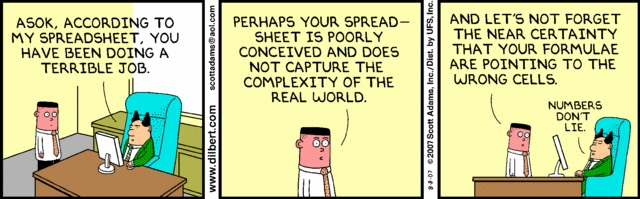
\includegraphics{dilbert-excel}
    \caption{\href{http://dilbert.com/strips/comic/2007-08-08/}{Dilbert on spreadsheets}, by Scott Adams. For a real-world illustration, find the `Reinhart and Rogoff' story online, or read some horror stories compiled by the European Spreadsheet Risks Interest Group (EuSpRIG):   \url{http://www.eusprig.org/horror-stories.htm}}%
    \label{fig:dilbert-spreadsheets}%
  \end{figure}

  A more balanced account would find some qualities to spreadsheet editors,%
  \footnote{See William Huber's answer to the CrossValidated topic ``\href{http://stats.stackexchange.com/a/3398/3582}{Excel as a statistics workbench}''.} %
   and using Stata will remind you of a few things that you might have already learnt from using these them. This will include using keyboard shortcuts to move around the interface and do things quicker, and will also include using functions like \texttt{if} or \texttt{mean} that you might have already used on spreadsheet cells.%
  %
  %

Statistical programming, on the other end, is probably new to you. Its general principle consists in composing a sequence of instructions that enables others to `replicate' your analysis. The current de facto standard in statistical programming is R, a free and open source software with excellent graphics support that lets you crunch numbers like a statistician would want you to: neatly, if at the cost of intuitiveness.%
  \footnote{\url{http://www.r-project.org/}} %
  %
  %

\newthought{Stata is a compromise} between these two worlds that lets you work on a single spreadsheet of data through a set of predefined and user-contributed commands. Its language is arguably more convenient than those developed by other solutions like SAS or SPSS, and its capabilities reach beyond those of more focused software, such as Epi~Info for epidemiology or gretl for econometrics.%
  %
  %

Stata has its own limitations: its graphics engine is not bad, but it is far from excellent, and despite being open to user-contributed commands, Stata is a commercial product with a price tag and a closed proprietary format. Finally, and although that can be seen as a feature of the software, Stata can only work on a single dataset at a time, because it works like an accountant's book, one page after the other.%
  %
  %

\newthought{This section} first covers some basic computer components. It then explains how to operate Stata from the command line, how to write code in the Stata language, and how to execute it by writing and `running' do-files, scripts of Stata code.%

We will use the `Standard Edition' (\textsc{se}) of Stata~12 that works on most current computers.%
\footnote{See the list of Stata products and compatible operating systems: %
  \url{http://www.stata.com/products/compatible-operating-systems/}}%
  %
  The keyboard shortcuts we provide are for \OSX (Mac) and Windows (Win). The installation procedures on both systems are almost identical:% 

\begin{description}

  \item[On \OSX] %
  %
  The entire Stata application folder should be located in the \texttt{Applications} folder. You should drag the Stata application icon to your Dock for quicker access. The \kbd{Cmd} (Command) key used in keyboard shortcuts is the `Apple' modifier key located left and right of the spacebar.%

  \item[On Windows] %
  %
  The entire Stata application folder should be located in the \texttt{Program Files} folder, or whatever your version of Windows calls it. You should drag the Stata application icon to your Taskbar for quicker access. The \kbd{Ctrl} key used in keyboard shortcuts is the `Control' modifier key located bottom-left of the spacebar.%

\end{description}

\index{Course!Requirements!Computer skills}%
\newthought{Learning Stata requires using a computer for research}, not just as a clever typewriter or as a Web terminal. This in turn requires that you practice using keyboard shortcuts and managing files, and implies that you have daily access to a usable computer that can connect to the Internet, read/write \PDF files and uncompress \ZIP archives.%

You might use computers routinely for many different activities, but your level of familiarity with some of the fundamental aspects of computers can vary dramatically. A reasonable level of familiarity with computers will help you with using Stata and completing assignments.%

Besides building up your scientific and statistical computer skills, there are extrinsic reasons to why you might want to pay some attention to computing in the current times. One aspect of the argument is that computer code is the effective institution that rules over digital communication.%
  \footcite{Lessig:2006} %
  The gist of the argument might be put as follows: %

\begin{quote}%
Digital technology is programmed. This makes it biased toward those with the capacity to write the code. In a digital age, we must learn how to make the software, or risk becoming the software. It is not too difficult or too late to learn the code behind the things we use—or at least to understand that there \emph{is} code behind their interfaces. Otherwise, we are at the mercy of those who do the programming, the people paying them, or even the technology itself.%
\footcite[p.~128]{Rushkoff:2010}%
\end{quote}

Another aspect of the argument is that, whereas states are gradually expanding their grip over free and private electronic communication, companies are gradually turning general purpose computers into focused commercial appliances that provide less and less control to the user over the technology.%
  \footcite{Doctorow:2011} %

% 1.3.1
%
\subsection{Working with computers}%
  %
  %
  \label{ch:computers}%
  \index{Computers}%
  %
  %

\index{Computers!Hardware and software}%
\newthought{Your computer's physical and electronic parts (hardware)} include input and output (I/O) devices like your keyboard and screen, a central processing unit (CPU) and memory storage, both as hard drive space and as ``live'' or ``virtual'' random access memory (RAM), which is used to read and write data more rapidly.%
  \footnote{Stata~11 or older will require that you manually allocate the memory space to store datasets. You are spared from doing that if you are using a later version of Stata.} %
  All components communicate with each other over a communication network called the bus.%
%

\newthought{The software layer of your computer} are the programs that you use to send instructions to the hardware layer. Your operating system provides an initial layer of software that you can then expand with additional programs like Stata to perform more specific tasks. The speed at which you can use your computer is determined by the amount of RAM that you have installed, by the speed at which you can read or write to your hard drive, and by the speed of your processor, the `CPU'.%
%

%
\paragraph{CPU (Central Processing Unit)}%
  \index{Computers!CPU (Central Processing Unit)}%
  %
  %

\newthought{The CPU performs arithmetic and logic operations on your computer data} and stores their intermediate results. It also controls how tasks are executed on your system by allocating them processor time to compute. If you live in the early twenty-first century, there is a fair chance that your laptop runs a multi-core processor with several linked microchips that can compute separate tasks in parallel.%

Your CPU operates at a given cycle speed, which is currently calculated in GigaHertz (GHz). The 2.53GHz Intel Core 2 Duo CPU that ships with the Apple MacBook Pro, for example, is a dual-core processor that ticks at the clock rate of 2.53 billion cycles per second. These cycles are used to process low-level program instructions that underlie the software that you use. That software might live on your computer or in the cloud.%
  \footnote{See, for instance, the OpenCPU project for statistical computing: \url{https://public.opencpu.org/pages/}}%

%
\paragraph{Logic gates and truth tables}%
  \index{Computers!Logic gates}%
  \index{Computers!Truth tables}%
  %
  %
  
\newthought{Your computer is made of digital circuits that implement logic gates}, such as the ones shown in Figure~\ref{fig:gates}. These gates provide the basic mathematic logic that is also used in the software layer of your computer, as when you make use of logical statements to manipulate your data in Stata.%
  \footnote{See Table~p.~\ref{tbl:logical-symbols} at p.~\pageref{tbl:logical-symbols}.}%
%

\begin{figure}[h]
  \begin{circuitikz}
    \draw (0,0) node[american and port,color=s1] (aand) {};
    \draw (2.5,0) node[european and port,color=s2] (eand) {};

    \draw (5,0) node[american or port,color=s1] (aor) {};
    \draw (7.5,0) node[european or port,color=s2] (eor) {};

    \draw (9,0) node[american not port,color=s1] (anot) {};
    \draw (12,0) node[european not port,color=s2] (enot) {};
  \end{circuitikz}

  \caption{The \texttt{AND}, \texttt{OR} and \texttt{NOT} logic gates in American (red) and European (blue) representations.}%
  \label{fig:gates}
\end{figure}

These logic gates allow your computer to understand basic truth tables, as with the union of two conditions \texttt{A AND B}, their intersection \texttt{A OR B}, or the negation of \texttt{A}, \texttt{NOT A}. Combinations of logic gates are then used to build electronic circuits with two stable states, a.k.a. ``flip-flops''. All data in a computer are stored in that form as binary digits.%
%

%
%
\paragraph{Bits and bytes}%
  \index{Computers!Binary digits}%
  %
  %

\newthought{A \emph{bit} is a single binary digit (0/1).} Modern processors use units of data, or ``words'', that go from 8 to 64 bits. A \emph{byte} is a series of eight bits and a ubiquitous standard in computer architecture. Given that a bit take two values, a byte can take $2^8=256$ values to express a number in the $0-255$ range, or to represent up to 256 characters.%

In a computer environment, larger arrays of bits and bytes provide more power to process and define whatever stuff you are dealing with. The current Unicode UTF-8 standard, for instance encodes text in several alphabets by using up to four bytes to define thousands of different characters. The same logic applies to graphics on a video game console.%

The current technological frontier puts your computer processor at either 32-bit or, for the most recent machines, at 64-bit; Stata~12 for Windows exists in both versions, whereas Stata~12 for \OSX works only on 64-bit processors. %
  \footnote{\url{http://www.stata.com/support/faqs/windows/64-bit-compliance/}}

%
%
\paragraph{Operating system}%
  \index{Computers!Graphical User Interface (GUI)}%
  \index{Computers!Operating system}%
  %
  %

\newthought{Your operating system (OS) manages your files, I/O devices, memory and networks.} It manages each application as a process, uses your hard drive to swap data in and out of virtual memory, and makes multi-tasking possible by switching very quickly between programs. Your OS also comes with a graphical user interface (GUI) that makes the computer usable by human beings.%

%
% 
% 0.3.2.
%
\subsection{Working from the command line} %
  \label{sec:cli}
  \index{Computers!Command Line Interface (CLI)}%
  \index{Stata!Command line interface}%
  %
  % graphical user interface
  % command line
  % example: sysuse lifeexp
  %

\newthought{This section explains how to run commands in Stata}, and the next one will explain how to organize them into a do-file. A list of all commands used in the guide appear in the index, and a list of all commands used in the course appear on the course wiki.%
  \footnote{\url{https://github.com/briatte/srqm/wiki/code}} %
For now, open the Stata program by double-clicking its application icon (Figure~\ref{fig:stata-icon}).

  \begin{marginfigure}
    
\includegraphics[width=.66\textwidth]{stata-icon}
    \caption{The Stata~12 icon.}
    \label{fig:stata-icon}
  \end{marginfigure}

Stata can be used either through its GUI, like most of the software that you use, or through a Command Line Interface (CLI), which presents itself as a terminal where the user types instructions to produce certain results. The latter approach is more versatile and forces you to write up your operations in the form of a script, which Stata calls a `do-file'. This file is a plain text file containing code written in the Stata language.%

We are going to explore Stata from the command line, which relies only on three windows: the Command line window, the Results window attached to it, and the Do-file Editor window. This minimal setup is shown below in Figure~\ref{fig:stata-ide}. We will not use any other element of the graphic user interface in this course, but feel free to explore Stata and learn about its other functionalities.%

\begin{figure}
  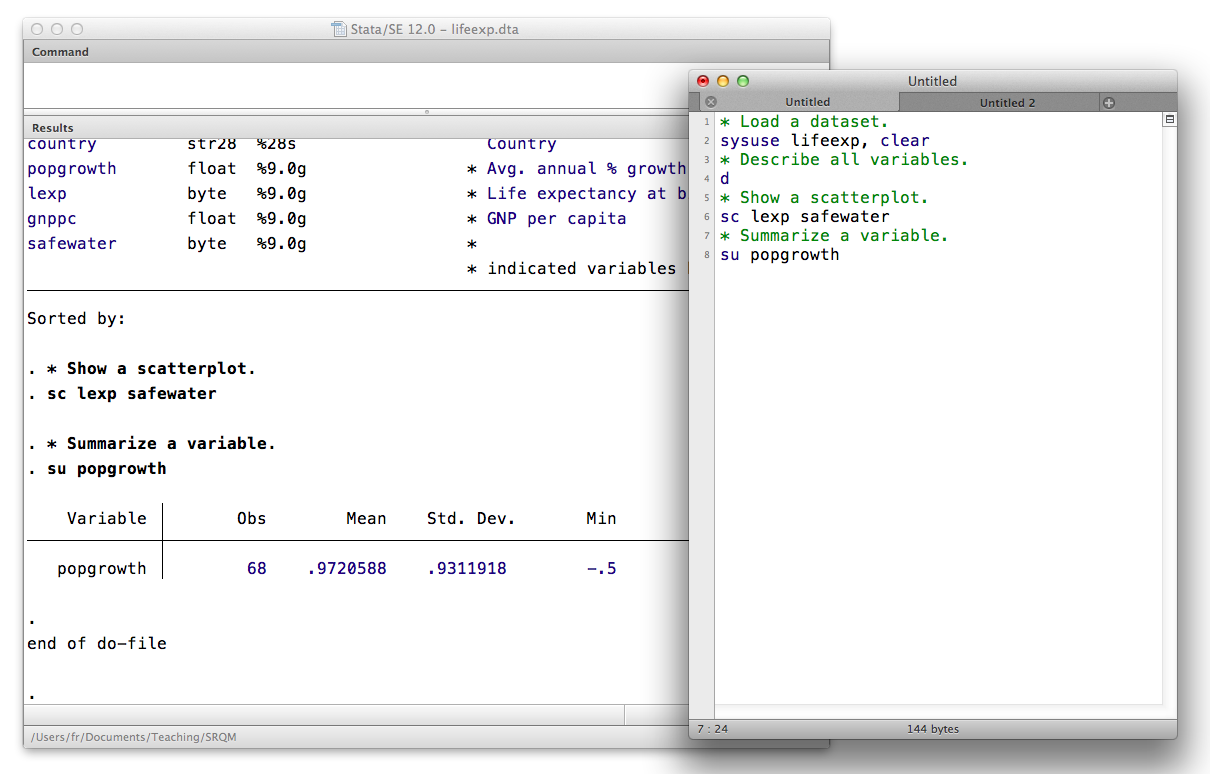
\includegraphics{stata-ide}%
  \caption{The Holy Trinity of Stata programming: the Command window (on top), the Results window (below it), and a do-file editor (in the background).}%
  \label{fig:stata-ide}%
\end{figure}

  \paragraph{Running commands}
  
  In Stata, focus on the Command window by clicking into it or by pressing \kbd{Cmd-1} (Mac) or\kbd{Ctrl-1} (Win). Type the following command and press \texttt{Enter} to run the command, which means to execute its code:%
    
  \begin{docspec}%
    \label{lifeexp}%
    sysuse lifeexp, clear
  \end{docspec}
    
  A Stata command is simply a line of code written on a distinct line of a do-file. If your command ran successfully, Stata will display its result:\\[1em]
    
    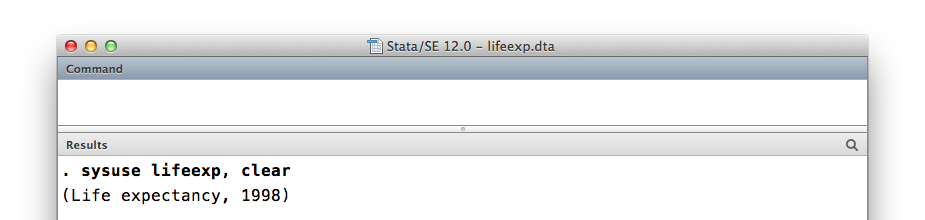
\includegraphics{stata-lifeexp-sysuse}\\[1em]

  Note that some commands produce `blank' output, which means that a command can be successfully entered and executed without printing any result. In this case, a simple \texttt{.} line dot will appear in the Results window, as to show that Stata encountered no problem while executing the command, and that it is ready to process another one.%
    %

  %
  %
  \paragraph{Fixing typos}%
      \index{Stata!Syntax}%

  Stata commands follow a strict syntax, and if you make a typo in a command, the software will return an error in red ink. In that case, you have to fix the issue by re-typing the command correctly. Try for example, to enter the following command:%
    
    \begin{docspec}
      summarizze popgrowth
    \end{docspec}%
    \marginnote{Examples with the \texttt{lifeexp} dataset continued from p.~\pageref{lifeexp}.}%
    
    The mistake is rather obvious here: the \cmd[su]{summarize} command should take only one `z':\\[1em]%
    
    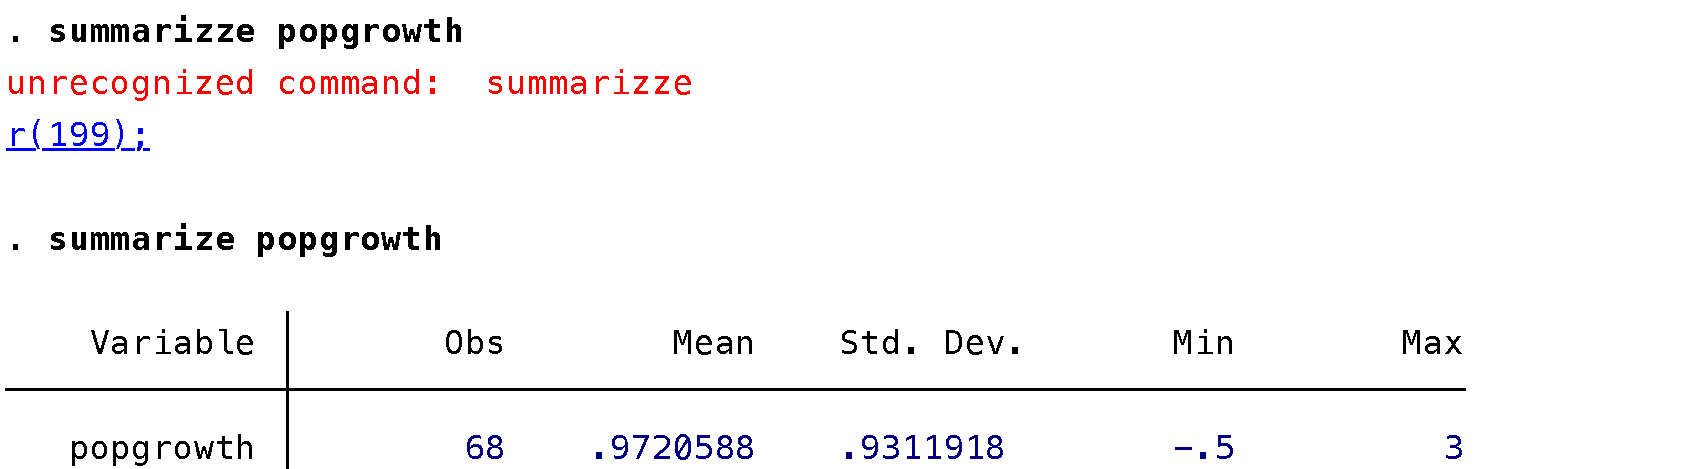
\includegraphics{lifeexp-sum-error-zz}\\[1em]
    
    If you need, as in this example, to correct a mispelled command, or to re-run a command that you have used earlier on, you should \textbf{press \kbd{PageUp} on your keyboard} to recall the previous command that you typed.%
    %
    \footnote{On laptop keyboards, \kbd{PageUp} is usually replaced by \kbd{Fn-UpArrow}. Past commands can also be examined in the Review window.} %
    %
    This allows you to fix your mistake by pulling the last command very quickly and correct only the typo, rather than having to type it again.%

    Here's another common mistake. Try the following in Stata:%
    
    \begin{docspec}
      Summarize popgrowth
      summarize POPGROWTH
    \end{docspec}

    In response to these commands, you will get more or less informative error messages. The issue here is that Stata commands are case-sensitive: the capitalized \texttt{Summarize} command is different from \texttt{summarize} command in lowercase. By that virtue, there is no variable called \texttt{POPGROWTH} in uppercase in the \texttt{lifeexp} dataset, but there is one called \texttt{popgrowth} in lowercase:\\[1em]%

    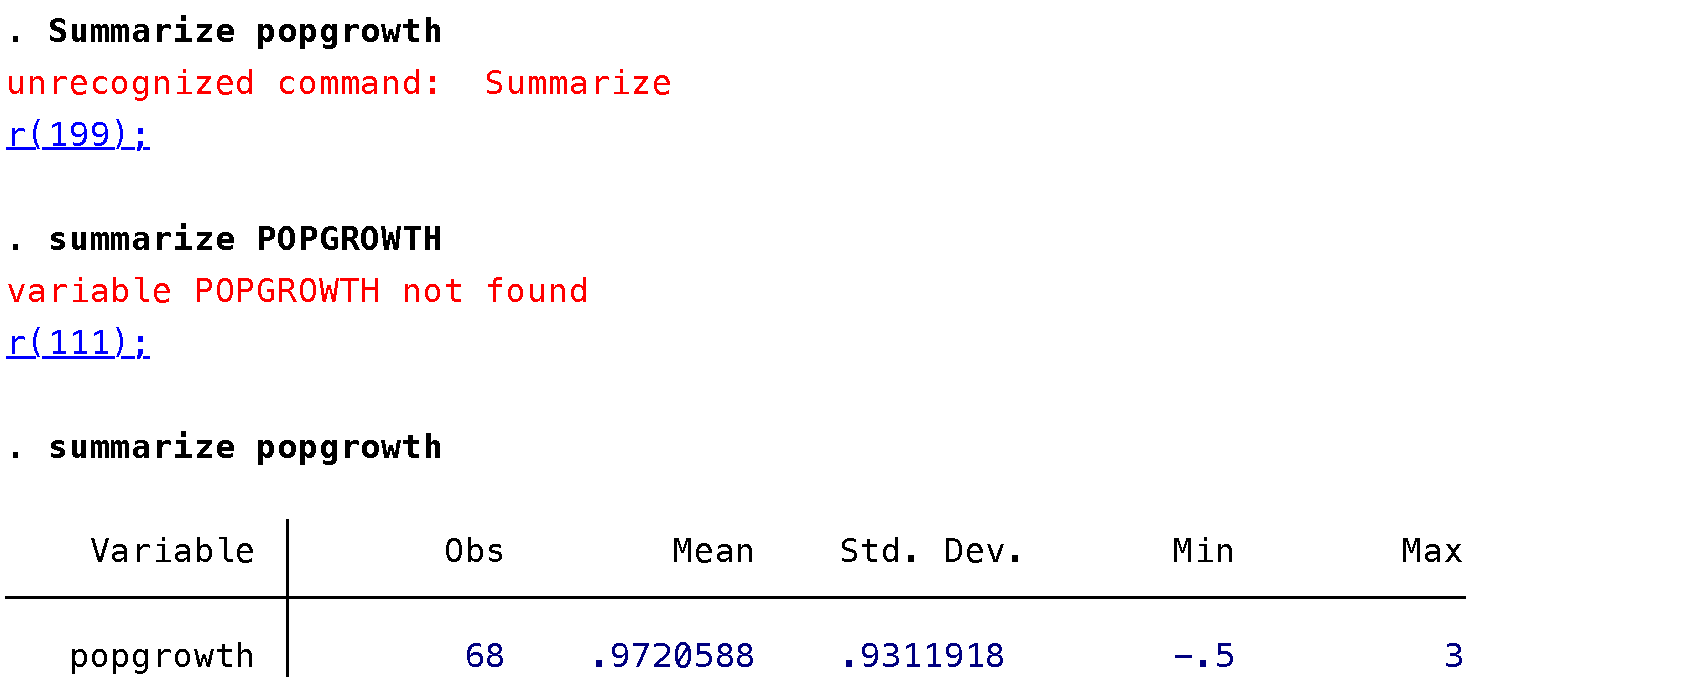
\includegraphics{lifeexp-sum-error-caps}\\[1em]
    
    Stata is usually operated in lowercase, although some variable names might show up in uppercase in some datasets. In order to keep things as straightforward as possible, avoid using uppercase yourself when naming variables.%
    
    %
    %
    \paragraph{Abbreviations}%
      \index{Stata!Syntax}%

    Most Stata commands can be abbreviated for quicker use. If you run the \statacode{help summarize} command, the help window will tell you that the \texttt{\underline{su}mmarize} command can be abbreviated to \texttt{su}. Type the following example in Stata to see how the language abbreviates:%
    
    \begin{docspec}
      * With a command:\\%
      summarize popgrowth\\%
      su popgrowth\\[1em]%
      %
      * With help pages:\\%
      help summarize\\%
      h su%
    \end{docspec}%
        \marginnote{Examples with the \texttt{lifeexp} dataset continued from p.~\pageref{lifeexp}.}%

  Note that the bottom lines show you how to open help pages with the single letter \texttt{h}, which is handy when you are often brought to verify syntax and read examples from the documentation. This guide shows commands that can be abbreviated in both forms, as with \cmd[su]{summarize}, which is shown in the example:\\[1em]%

    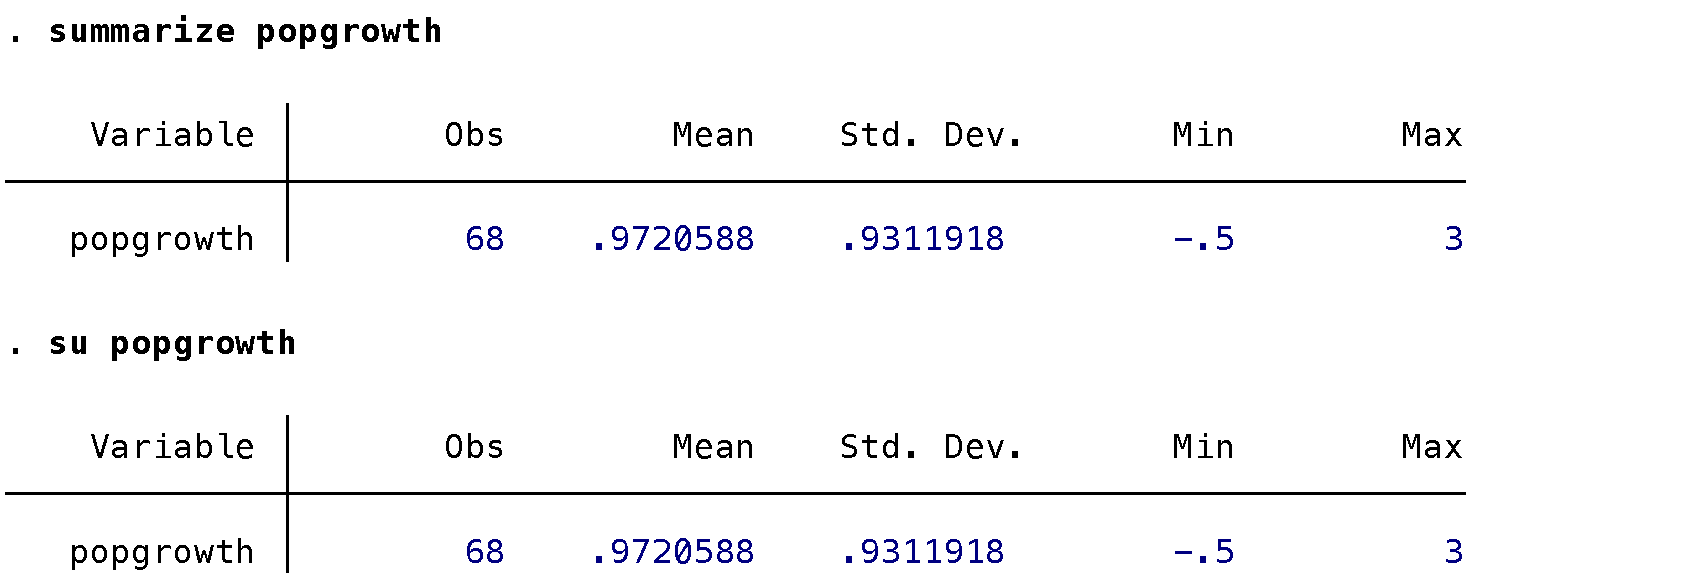
\includegraphics{lifeexp-summarize}\\[1em]

  Abbreviations exist for most commands and come in handy especially with commands such as \cmd[tab]{tabulate}, \cmd[d]{describe} or even \cmd[h]{help}. They also work for options like the \coab{d}{detail}{summarize} option for the \cmd[su]{summarize} command:\\[1em]%

    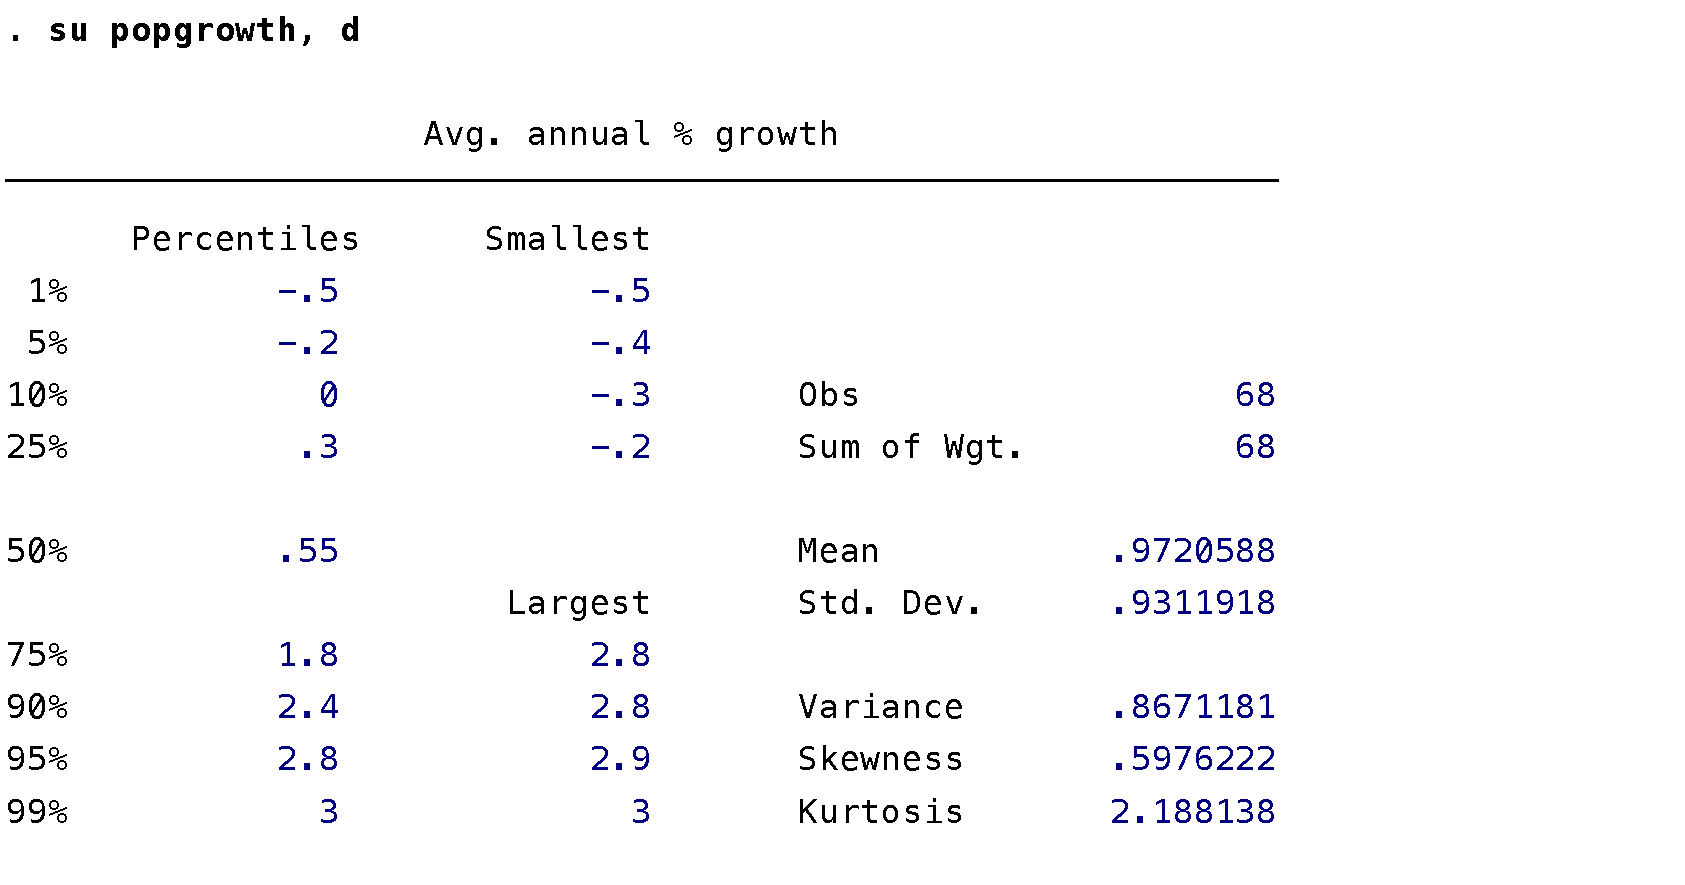
\includegraphics{lifeexp-summarize-d}\\[1em]
  
    %
    %
    \paragraph{Using help files}%
      \index{Stata!Help files}

    If you cannot find the right syntax or option for a command, turn to the technical documentation for precisions and examples of any given command. Use the \cmd[h]{help} command to access it in Stata,%
        \footnote{Stata help is also available online: \url{http://www.stata.com/help.cgi?help}.} %
        as in these examples:%

    \begin{docspec}
      * Help for the -summarize- command.\\
      help summarize\\[1em]
  
      * Help for the -lookfor- command.\\
      help lookfor
    \end{docspec}

    Getting to use the Stata help pages is a course objective in itself: even experienced Stata users use help pages on a daily basis. The details on each option and the final examples are often very useful in learning to use some commands efficiently.%

    \newthought{You can find additional help} for Stata in the series of manuals and handbooks published by Stata Press. Appropriate references for this course are the ``Getting Started'' manuals, which cover the same basic operations as this guide.%
      \footnote{\url{http://www.stata-press.com/}} %
      StataCorp also publishes the \emph{Stata Journal}, a blog and a video channel of Stata tutorials.%
      \footnote{\url{http://blog.stata.com/2012/09/26/stata-youtube-channel-announced/}}
  
    The course website features a list of additional online resources to learn Stata. One particularly interesting resource for beginners is the Stata video series by the LSE Methodology Institute.%
      \footnote{\url{http://www.youtube.com/user/MethodologyLSE/videos?query=stata}} %
      Stata users also share questions and answers on Statalist%
      \footnote{\url{http://stata.com/statalist/}} %
      and on Stackoverflow.%
      \footnote{\url{http://stackoverflow.com/questions/tagged/stata}}

%
%
\paragraph{Installing commands}%
  \index{Stata!Packages (additional commands)}%

Stata can install additional commands written by users with programming skills. New commands can be installed by downloading packages from the \SSC server with the \cmd{ssc install} command, which is used at a few points in this guide to install some of these packages. You can install the \cmd{fre} command right away by typing the following command:%
  
\begin{docspec}
  ssc install fre
\end{docspec}
  
Unless you are offline or already have installed the \cmd{fre} package, you should get a few result lines indicating where the package was installed on your hard drive:\\[1em]%
  
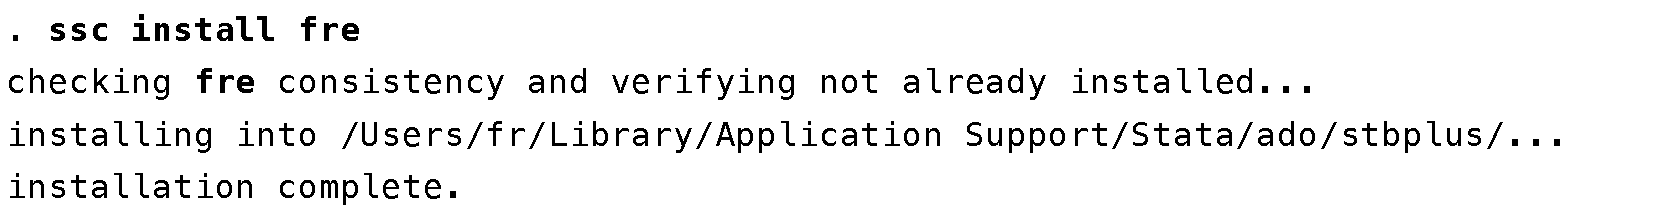
\includegraphics{ssc-install-fre}\\[1em]
  
Other handy user-contributed commands will be installed as part of the course setup that you will run in the next section.%

%
%
% 0.3.3
%
\subsection{Working from a do-file}%
  \label{sec:do-files}%
  \index{Stata!Do-files}%
  \index{Replication|seealso{Stata!Do-files}}%
  %
  % command execution
  % comments
  % log
  %

\newthought{When you run Stata commands} to explore a dataset, you are programming `on the fly', typing commands directly into the Stata command line to get quick results. But when you want to structure a complete analysis of your data, you need to record your commands to a script, which is a plain text file containing Stata code. An important part of your work in this course will therefore be to code your analysis into a script.%
%

Coding your analysis is meant to provide yourself as well as others with the means to \emph{replicate} your analysis. Maintaining a record of your operations—and commenting them inside as well as outside the code—will not only ensure that others can read and reproduce your work, but also that \emph{you} will be able to remember, in a few months or so, what you precisely ended up doing on your project. In this course as in many research settings,%
  \footnote{See \citeauthor{King:1995}'s article, \citetitle{King:1995}, and Nicole Janz's blog for more illustrations: \url{https://politicalsciencereplication.wordpress.com/}} %
  you will be required to bundle your Stata code with your analysis, so that the findings of your research project can be replicated by others. %

\newthought{Stata scripts} end with the \ext{.do} extension and are called \textbf{do-files} (Figure~\ref{fig:stata-do-icon}).%
  \footnote{Stata do-files will usually show as plain text in your Internet browser; if the browser adds a \ext{.txt} extension to a do-file when downloading it, make sure that you rename the file to \ext{.do} for Stata to recognize it as a do-file.} %
  %
  It will be one of your main missions throughout the course to learn how to structure and to write such a document. You will be given plenty of examples through a new course do-file every week, and the short vignette that follows will show you some essential aspects of working in Stata from a do-file.%

\begin{marginfigure}
  
\includegraphics[width=.66\textwidth]{stata-do-icon}
  \caption{Stata~12 do-file icon.}
  \label{fig:stata-do-icon}
\end{marginfigure}

%
%
\paragraph{Creating a do-file}

Type \cmd{doedit} in the Command window to open a blank Stata do-file, which is your first piece of draft Stata code. Let's write a few lines into it:%

\begin{docspec}
  * François Briatte, first do-file\\[1em]%
  %
  * Load UN data.\\%
  sysuse lifeexp, clear\\[1em]%
  %
  * Describe the data.\\%
  d\\[1em]%
  %
  * Summarize life expectancy\\%
  su lexp\\[1em]%
  %
  * Scatterplot.\\%
  sc lexp safewater\\[1em]%
  %
  * ttyl\\
\end{docspec}

Here are step-by-step instructions to the code:

\begin{enumerate}
  \index{Stata!Comments (code)}%
  \item First type in your name, preceded by an asterisk and a space. You will notice that the line will turn green, to indicate that it is a \textbf{comment}. Comments are for human readers of the code and are not evaluated by Stata, just passively printed to the Results window.%
  
  \item Now add the \cmd{sysuse} command that asks Stata to load a demo dataset in memory, removing any previous unsaved data. If you have run the previous examples, the same dataset will be loaded again.%
  
  \item Finally, add the \cmd[d]{describe} command to list the variables, the \cmd[su]{summarize} command to inspect the life expectancy variable, and the \cmd[sc]{scatter} command to produce a plot of the relationship between life expectancy and access to safe water.%
\end{enumerate}

Stata shows the code of your do-file in monospaced font with line numbers (so that you can easily navigate long documents) and colored syntax (so that you can distinguish syntax elements). The do-file editor should look like Figure~\ref{fig:hello-world-draft} on my system, which also highlights the currently selected line:%

\begin{figure}%
  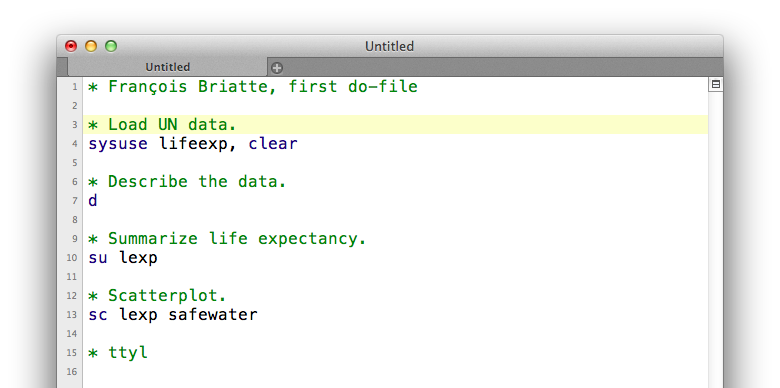
\includegraphics[width=\textwidth]{hello-world-draft}%
  \caption{A draft do-file using the \texttt{lifeexp} dataset.}%
  \label{fig:hello-world-draft}%
\end{figure}


\index{Stata!Comments (code)}%
\newthought{Every Stata command requires to be typed on a separate line.} You can skip lines and add whitespace in your code to improve its readability. Most importantly for that purpose, make sure to leave informative comments in your code, to explain how you designed your analysis.%

Increasing the readability of your research project is a requirement in courses that set the emphasis on data analysis. The general idea is to consider your code as a communication device with your peers, like a music sheet or as some other form of composition.%
  \footcite{WickhamGrolemund:2013} %  

\index{Programming!Literate programming}%
\newthought{Making your code readable by others} implies adding a `literate' component to it. This involves including some documentation of what your code does with the code itself, in order to help a human audience to read through your different files and functions.%
  \footnote{\url{http://www-cs-faculty.stanford.edu/~knuth/lp.html}} %

In your own work, you will be required to include short comments in your code to help the reader understand your analysis. Your code will also provide some general information such as the author(s), date and title, in an introductory header.%

\paragraph{Opening and saving do-files}

\newthought{Stata code is saved as plain text} into \ext{.do} files. Stata can open as many do-files as you need in a tabbed window environment, called the Stata do-file editor. You will have to work with course do-files and to write your own for your research project.%

Once you are done copying and editing the demo code from above, use \kbd{Cmd-S} (Mac) or \kbd{Ctrl-S} (Win) to save the do-file as \filename{draft.do} in your \code folder, where you should keep all your do-files within the \SRQM folder.%

Close your first draft and return to the Stata Command window. If you have saved your draft as \filename{draft.do} into the \code folder, as requested, then Stata will be able to open it with the following command:%

\begin{docspec}
  doedit code/draft
\end{docspec}

The \cmd{doedit} command opens do-files, and the \texttt{code/draft} argument is the short form of \texttt{"(your working directory)/code/draft.do"}, a file path that should lead Stata to open the do-file that you just saved. Note that \hlred{\textbf{opening a do-file by double-clicking it is not recommended}, because Stata will quietly change the working directory to the location of the do-file,} and you will have to set the working directory back to being the \SRQM folder.%
  \footnote{The same problem will arises if you open datasets by double-clicking it.}

Similarly, \hlred{\textbf{be careful when you download a do-file}, because your browser might add a \ext{.txt} extension to it}, in which case you will have to to rename the file by turning its file extension back to just \ext{.do} to open it correctly in Stata. Using the ``Save As'' contextual menu option of your browser can fix the issue, as shown in Figure~\ref{fig:save-as} with Google Chrome on \OSX.%

\begin{figure}
  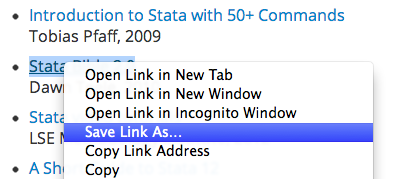
\includegraphics[scale=.5]{images/macosx-save-as.png}
  \caption{The ``Save Link As…'' option in Google Chrome for \OSX.}
  \label{fig:save-as}
\end{figure}

\paragraph{Running do-files}

\newthought{Having reopened your do-file}, click anywhere on line 2 of your draft do-file and then press \kbd{Cmd-L} (Mac) or \kbd{Ctrl-L} (Win) to select it in full. Then, press \kbd{Shift+DownArrow} or \kbd{Shift+UpArrow} to select the line below or above it.%

Finally, press \kbd{Cmd-A} (Mac) or \kbd{Ctrl-A} (Win) to select all three lines. These keyboard shortcuts show you how to quickly select one or more lines from your code: make sure to memorize them, as they will come in very handy.%

To execute the do-file, press \kbd{Cmd-Shift-D} (Mac) or \kbd{Ctrl-D} (Win). The first line is a comment, as indicated by the asterisk at the beginning of the line, so executing it will not accomplish anything: Stata will just print it to the Results window.%

The second and third lines of your do-file will be printed to the Results window with their respective results. The \cmd{cd} command should print the path to your \SRQM folder, and the \cmd{di} command will print a `hello' message, as shown in Figure~\ref{fig:hello-world-result}.%

\begin{figure}%
  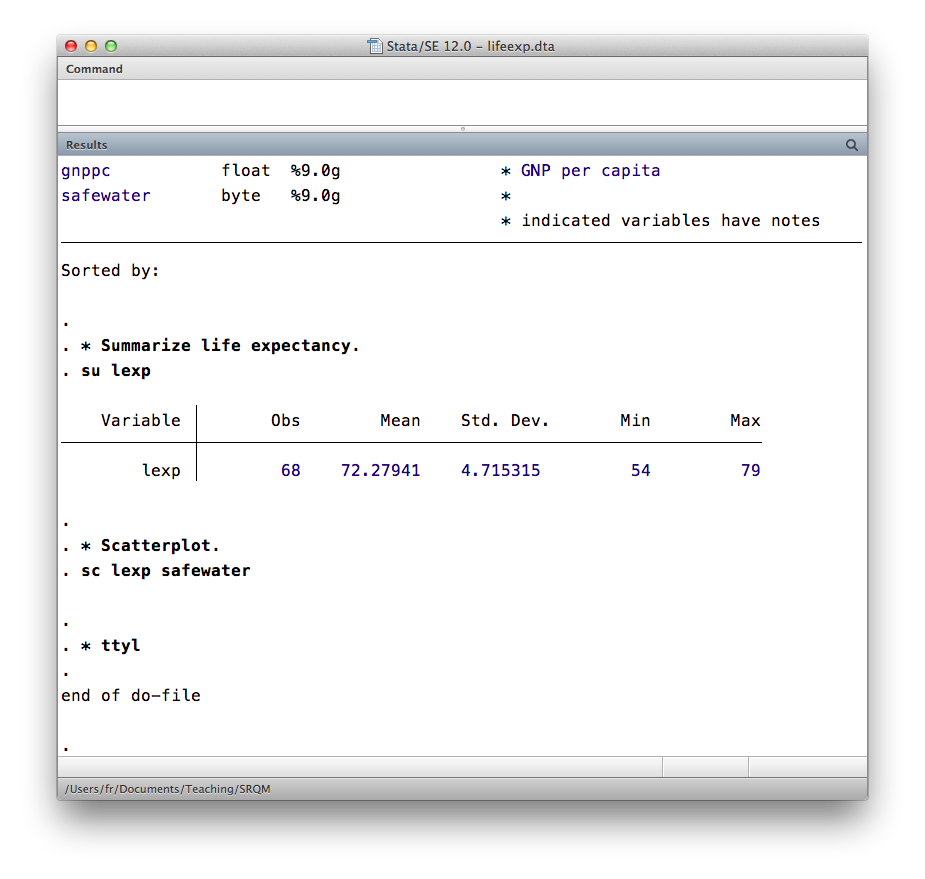
\includegraphics[width=\textwidth]{hello-world-result}

  \caption{`Hello World' in Stata.}
  \label{fig:hello-world-result}
\end{figure}

More generally, to execute (or `run') some code, open its do-file, select any number of lines, and ppress \kbd{Cmd-Shift-D} (Mac) or \kbd{Ctrl-D} (Win). You will practice executing Stata code when we go through the course do-files in class.%

\hlred{\textbf{Important:} check your commands for typos and syntax errors.} If your code fails to execute, Stata will send some red ink to the Results window. Check the code against the correct syntax, looking for forgotten (or extra) letters or spaces.%

\hlred{\textbf{Important:} be careful with copy-pasting to the Command window.} Copy-pasted commands that contain line breaks (\cmd{///}), for example, will not work properly. This point is covered again in the first course do-file.%

\hlred{\textbf{Tip:}} start using keyboard shortcuts as early as possible. For example, during class, you will often need to switch from a window to another one (between a do-file and its results). This can be done from the keyboard: use \kbd{Cmd-`} (Mac) or \kbd{Alt-Tab} (Win). Have a look at the `Window' menu for shortcuts to specific windows of the Stata interface.%

\paragraph{Logging your work}

The log is a text file that, once open with the \cmd{log} command, will save every single command you enter in Stata with its results to a text file. Systematically logging your work is good practice, even when you are just trying out a few things. Logs are useful when you have to read through your work again, share it with someone, or keep dated copies of your results.%

To open a log, type \texttt{log using} followed by a file name ending in \ext{.log} to produce a plain text file. Close a log with the \texttt{log close} command, optionally followed by the name of the log if you added one to it the \opt{name}{log} option. You will find examples of \cmd{log} commands at the very beginning and at the end of the course do-files.%

\index{Programming!Machine readability}%
\newthought{Your log should be produced as a plain text file} because these files are readable in any computer environment and can therefore be parsed and interpreted everywhere. The same applies to your code and to your data: using plain text formats will ensure that everyone will be able to read it.%

When your analysis uses quantitative data, you are often given a choice between an application-specific format, which is the \ext{dta} format in Stata, and a machine-readable format like \ext{csv}. The course uses the Stata format, but if you produce datasets on your end, maximize their portability by saving them to comma-separated values (\ext{csv}) format.%

\paragraph{Exiting}

When you are done with your work, just quit Stata like you would quit any other program. Stata will ask you whether you want to save your changes: \textbf{say no}. In this course, you will \hlred{never save any changes to the original datasets}: keep the teaching material intact at all times, so that it can be used throughout the semester.%
    %
    \footnote{If you ever alter a course dataset by saving it with modifications, quit Stata and delete its \ext{.dta} file in the \data folder. When you reopen Stata, the course setup will restore a pristine copy of the data from the \ZIP archive.}%

\newthought{The nerdy way to quit Stata} is to quit from the command line. A first optional step is to manually close all opened logs:%

\begin{docspec}
  * Close all open logs.\\%
  log close \_all
\end{docspec}

The \cmd{exit} command with the \opt{clear}{exit} option then erases any data in memory and quits:%

\begin{docspec}
  * Enjoy your day.\\%
  exit, clear
\end{docspec}
%
%
% 1.3 course setup
%
%
% 1.2
%
\section{Coursework}%

\newthought{The approach to social science} that we follow in this course is driven by a dual logic of inquiry: we start with the description of quantitative data, and we end with its analysis through statistical models. The procedures involved in this process are computational and require some technical knowledge of computers and mathematics.%
	%
	%

	%%% They’re someone who can ask and answer questions about and with data.
	%%% http://www.analyticstory.com/hadley-wickham/

	%%% I A key principle in applied statistics is that you should be able to connect between the raw data, your model, your methods, and your conclusions

	%%%%Controlled experiments are the gold standard, but I never do them!

%%% I (Some) computer scientists' view: we don't need controlled experiments; we can automatically learn from observational data

%%% I Psychologists' view: each causal question requires its own experiment

%%% I Observational scientist's version: each causal question requires its own data analysis

%%% Sample surveys (for the problem of extending from sample to population)

%%% Descriptive observational research (for the problem of modeling complex interactions and response surfaces)

%%%Political science is largely an empirical discipline. That is, most of us studying politics do so because we are motivated by real world political events, either historical, current, or even events yet to happen. We want to know why these events happen and how to make sense of them. Political science trys to answer these questions in a rigorous way. Data analysis is thus a critical component of political science, serving two important purposes: (1) providing numerical descriptions or summaries of political phenomena, facilitating comparisons across time, countries, states, people, etc; (2) testing theories, models and hypothesis about politics.


% All this is to say that this class involves a little math. Or, as I like to put it, this class is ‘‘techie for fuzzies’’: an introduction to the way political scientists use the tools of statistics to rigorously understand political events. I assume virtually zero mathematical background on your part, either because you didn’t take math in high school or because you’ve forgotten it. I assume no prior background with using computers for data analysis. The classes will have a heavy ‘‘show-and-tell’’ feel to them, where I will use statistical software to do data analysis.

%%%forecast the effects of interventions, the trajectory of existing trends, and the likely strategies

%%% http://understandingsociety.blogspot.fr/2009/01/predictions.html

% 1.2.1
%
\subsection{Course outline}%
  \index{Course!Outline and readings}
	%
	%

\newthought{This course} follows the standard regulations of Sciences Po, \ie, attendance is compulsory, every class comes with homework and readings, and plagiarism on any element of coursework is strongly sanctioned. Please turn to your academic regulations for more details on any of these topics.%

The course itself is organised in twelve two-hour sessions that run over a single semester. Its content is structured around three teaching goals:%

\begin{enumerate}
  
  % 1. Statistics

	\label{sec:textbooks}%
	\index{Course!Readings}%
  \item The course covers some \textbf{essential aspects of statistical analysis}, from describing variables to running regression models.%
  
  This learning objective requires that you read from textbooks that apply fundamental statistical theory to social science research. The primary textbook for this course is \citetitle{Urdan:2010a}\footcite{Urdan:2010a}, one of the shortest and most effective introduction to the course topics. %
	
	Towards the end of the class, we turn to \citetitle{FeinsteinThomas:2002d}\footcite{FeinsteinThomas:2002d}, a clearly worded introduction to quantitative methods for qualitatively-minded social scientists, for additional clarifications on regression modelling.%
  
	\index{Course!Syllabus}%
  Both textbooks appear in the course syllabus%
		\footnote{\url{https://github.com/briatte/srqm/blob/master/course/syllabus.pdf?raw=true}} %
    as well as in the final bibliography of this document. Please read the course syllabus in full at that stage, and copy the reading schedule to your agenda.%
		
  The textbook readings for this course will give you a more detailed view of statistics than this guide can provide. Furthermore, since the course slides are mostly trivia taken from the course blog,%
  \footnote{\url{http://srqm.tumblr.com/}} %
    you really have no other choice than to take the time to go through the assigned readings. The weekly readings appear at the beginning of each section of this guide, in the course syllabus, and on the course website.%

  % 2. Stata

  \item The course also explains \textbf{how to operate Stata} for basic data analysis and visualization.%

    \newthought{There will be one Stata do-file to study per week of class.} We will start looking at the do-file in class, and you will be asked to finish replicating it at home. Some online tutorials and Stata Press handbooks, like the recent one by \citeauthor{Mitchell:2012a} on applied regression,\footcite{Mitchell:2012a} can also be used as additional companions.%
		\footnote{See an indicative list of tutorials and books on the course website and on the course wiki: \url{https://github.com/briatte/srqm/wiki/stata}} %
    
    The do-file for the first week covers basic Stata settings and data exploration commands. It will show you how to start exploring the course datasets. Your weekly mission is to replicate the do-file of the current session. After running through the setup described in Section~\ref{sec:course-setup}, the following command will open the do-file for Week~1:%

      \begin{docspec}
        doedit code/week1.do
      \end{docspec}

     \newthought{Read through the do-file and execute (run) its commands sequentially}, reading the comments that precede each block of code. This practice (replicating the course do-files) will show you how to code various things in Stata, which will become handy when you start writing code for your own research project.%
    
     The baseline advice to survive the computing component of the course is very simple: practice by reading and writing code every week of class. If this is going to be the only time in your student life where you get to write statistical code, make sure that you get the most out of it. There is a fair chance that you will be offered to use that skill one day.%
  %

  % 3. Research

  \index{Course!Research projects!Final paper}%
  \item The course finally works assists students to work in pairs over \textbf{small-scale research projects}, on which the grading for the course is based.%
  
    Each student pair submits two draft versions of their empirical analysis (Stata code) and analytical report (research paper) during the semester, and one final version of their at the end of the class. The steps that each student pair needs to take throughout the semester to complete their research projects can be summarised as follows:%

    \begin{itemize}
      \item \textbf{setting up your computer} to follow the course and access the teaching material from the \SRQM folder (Weeks~1--2; Section~\ref{ch:intro});%
      \item \textbf{registering a research topic} with a student partner from your class in the course projects list (Weeks~2--3);%
      \item \textbf{exploring the course datasets} to find variables related to your research topic and select some variables of interest (Weeks~3--4; Section~\ref{ch:data});%
      \item \textbf{submitting your first draft} that presents the topic, the data the distributions of the variables under scrutiny (Weeks~4--5; Section~\ref{ch:distr});%
      \item \textbf{revising your draft} and resubmitting it with additional significance tests of associations in the data (Weeks~5--8; Sections~\ref{ch:asso} and \ref{ch:ols}); and%
      \item \textbf{submitting your final paper} in which you model your data with linear or logistic regression (Weeks~9--12; Sections~\ref{ch:lin} and \ref{ch:log}).%
    \end{itemize}

    \newthought{The deadline} for the first draft is generally set to mid-term (Week~6). The deadline for the revised draft is generally set to Week~10. The deadline for the final paper is generally set to one week after the last course session. In order to make all groups benefit from the challenges that arise in each project, you will be offered to submit questions to collective FAQs before every deadline.%
    %

    \hlred{Exact deadlines and all other project instructions are covered exclusively in class, which is why you should \textbf{attend every week and catch up if absent}.} The course sessions are cumulative: you cannot just skip one as if it had never happened. Your stress and workload \emph{will} increase if you skip a week with the hope of catching up later, and you will \emph{not} be able to fix your project if you let it rest.%
    %

		\newthought{Please read} \citeauthor{White:2005a}'s \citetitle{White:2005a}%
      \footcite{White:2005a} %
      for a refresher on how to write an empirical research paper. If you have never carried empirical research before, please also turn to \citeauthor{BoothWilliams:2003v}'s \citetitle{BoothWilliams:2003v}%
      \footcite{BoothWilliams:2003v} %
      for a detailed explanation on how to prepare a research project. All other teaching material for the research projects paper templates and example papers, is distributed through Google Documents in class.%
    % ^^^^^^^ 
    % replace by internal Google Documents support at Sciences Po (2013)?

		You are encouraged to use your research paper for other purposes than this course: think of it as work that you will be able to add to your student portfolio. Some students have used the coursework from this class to draft \textsc{Msc} dissertations, working papers or essays from other classes on research design and research methodology. Other students have used Stata for other projects in organizations that either consume or produce data.%
      \footnote{Examples from past years include a lot of consulting work on urban areas, research on land law and its effects on economic development, and estimating the number of refugees in a given geographical area to help plan the work of a nongovernmental organization.}%
		%
    
\end{enumerate}

% 1.2.2
%
\subsection{Course setup}%
	%
	%
	\label{sec:course-setup}%
	\index{Course!Setup}%
	%
	%

	\newthought{This section} explains how to set up Stata to follow the course. It assumes very little knowledge of computers or Stata, but please make sure that you have read through the previous section first. \hlred{\textbf{Make sure that you successfully set up your computer} for the course, and that you know how to run the setup again if needed.}%

	The setup below has been tested on Sciences Po workstations equipped with Stata~11. You might run into issues with this setup only if you use a computer with heavy user restrictions or with a really old copy of Stata. Please let us know if the setup fails.%
    \footnote{GitHub users can report issues on the course repository: \url{https://github.com/briatte/srqm/issues}}%
	
	% i
	%
	\paragraph{Get the teaching material}%
		\label{sec:teaching-pack}%
		\index{Course!Teaching material}

	\newthought{The `Teaching Pack' for this course comes in a single folder,} called the \SRQM folder, which you will have to access very frequently inside and outside class. Download and unzip the folder from its webpage%
		\footnote{\url{http://f.briatte.org/srqm/}} %
		or use the copy provided in class, and keep the \ZIP archive of the folder as a backup.%
		
	\hlred{Move the \SRQM folder to a \textbf{stable location} that you can easily locate on your hard drive, and keep it at that same location throughout the entire course.} Most users deal with this requirement by putting the \SRQM folder with the rest of their study files and then creating an alias to it on their Desktop.%
	
	Use any method that does not involve clicking for two full minutes to access the \SRQM folder, and do not rename its enclosing folders. For simplicity, leave the folder name to \SRQM for the class, and rename it to whatever you like at the end of the semester.%
	
	At that stage, \textbf{check the contents} of the \SRQM folder. The \SRQM folder contains the entire course material, minus the copyrighted textbooks and Stata software. The full contents of that folder, shown in Figure~\ref{fig:srqm-folder}, must stay available on your hard drive during the entire course.%
		%
		%

		\begin{figure}%
		  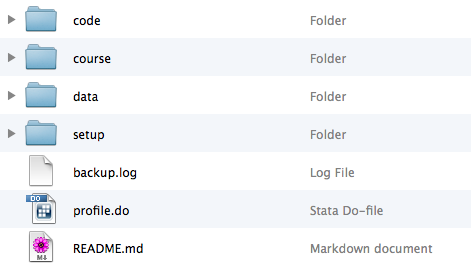
\includegraphics[width=\textwidth]{srqm-folder}
      
		  \caption{The contents of the \SRQM folder should match %
			this screenshot from a \OSX setup.}
		    \label{fig:srqm-folder}
		\end{figure}
		%
		%
		
	The \course folder contains the course slides and syllabus, as well as this guide. The \data folder contains a selection teaching datasets, and the \code folder will host the course do-files (covered below at p.~\pageref{sec:do-files}). The \setup folder and \filename{profile.do} files provide additional course functionalities. All folders are required for the course to roll out properly.%
		%
		%	\index{Computers!File and folder paths}%

	\index{Computers!URLs}%
	You need to understand the file structure of the course to understand how Stata will locate its files and folders from their \textbf{paths}. The path to the \SRQM folder, for example, might look like this on \OSX:\\[1em]%
	
	\begin{docspec}
		/Users/fr/Documents/Teaching/SRQM
	\end{docspec}
	
	The beginning of that path is often abbreviated through a tilde, so that \texttt{~/} designates the user folder. Stata understands that `tilde expansion' notation. Stata for Windows also understand paths with \texttt{\textbackslash} backslashes slashes as used in Windows, where the path generally starts on the \texttt{C:} drive:%

	\begin{docspec}
		C:\textbackslash{}Users\textbackslash{}Ivo\textbackslash{}Desktop\textbackslash{}SRQM
	\end{docspec}
	
	Once a folder has been set as the \emph{working directory}, Stata can locate files and folders from within it by using relative paths. The example below shows the relative path of the \texttt{nhis9711.dta} dataset in the \texttt{\data} folder:\\[1em]%
	
	\begin{docspec}
		/Users/fr/Documents/Teaching/SRQM/\hlred{\underline{data/nhis9711.dta}}
	\end{docspec}

	File paths are used in Stata to open and save datasets and other types of files. In some cases, it is also possible to open files from online sources by specifying their \URL. A \URL is an Internet address like the one that brings up the course webpage.%
		\footnote{\url{http://f.briatte.org/teaching/quanti/}}%
		%
		%
	
	We will use file paths and \URL\ s extensively throughout the course, so make sure that you understand both. I do my best to keep things tidy on my end by using Internet shortlinks and simple, informative folder and file names for the course material. You will have to do the same on your end.%
		%
		\footnote{For instance, you will be required to submit your work under a specific group name that includes your family names in alphabetical order.}%
		%
		%

	% ii
	%
	\paragraph{Set your working directory}%
		\label{sec:working-directory}%
		\index{Course!Teaching material}

  \newthought{Open Stata.} \OSX users can simply double-click the application icon. \hlred{\textbf{Windows users} will have to run Stata with administrator privileges: do this by right-clicking the Stata application icon then selecting `Run as Administrator.'} This will allow Stata to save files anywhere on the hard drive, which is required only for this setup.%
	 
	You are now going to set the working directory, which is the folder in which Stata opens and saves files by default. From the `File' menu, choose `Change working directory...', then select the \SRQM folder and press \texttt{Enter}. You will see something like the following printed in the Results window, that is, a folder path ending with the \SRQM folder:\\[1em]%
	
		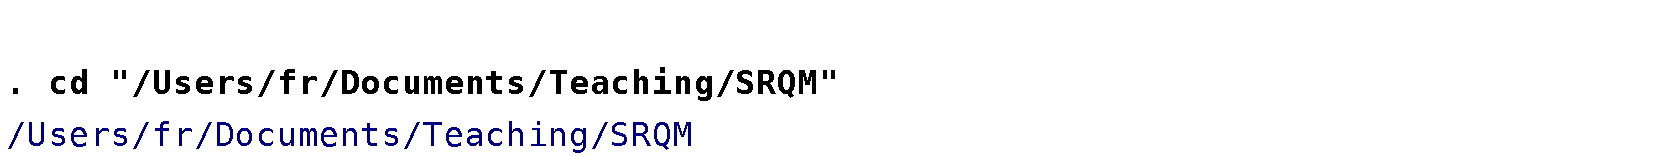
\includegraphics{srqm-cd}\\[1em]

	As the code output shows, the Stata command to do what you did through the `File' menu is \cmd{cd}, for `\underline{c}hoose \underline{d}irectory,' followed by the path to the desired folder. Now that you have learnt a Stata command, try it out by typing the following lines in the Command window and pressing \texttt{Enter} to execute each line:%
	
	\begin{docspec}
		cd ..\\
		cd SRQM
	\end{docspec}
	
	The first command, \texttt{cd ..}, changes the working directory to the enclosing folder, which in my case is the \texttt{Teaching} folder. The second command returns to the \SRQM folder and makes it the working directory again:\\[1em]%
		
	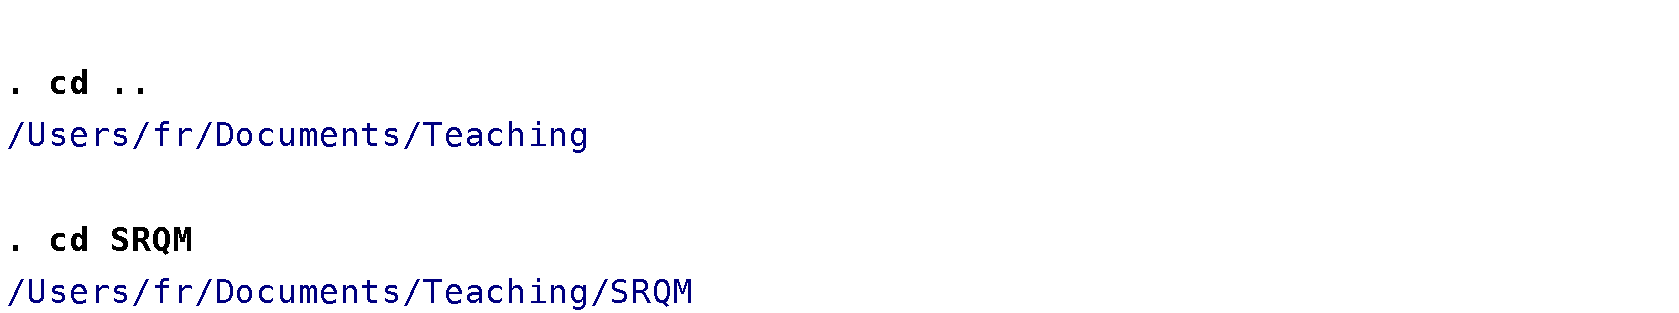
\includegraphics{srqm-cd-back}\\[1em]
	
	You can also list the contents of the working directory with the \cmd{ls} command. The example below will show the full contents of the \SRQM folder with detailed file information:%
	
		\begin{docspec}
			ls
		\end{docspec}

		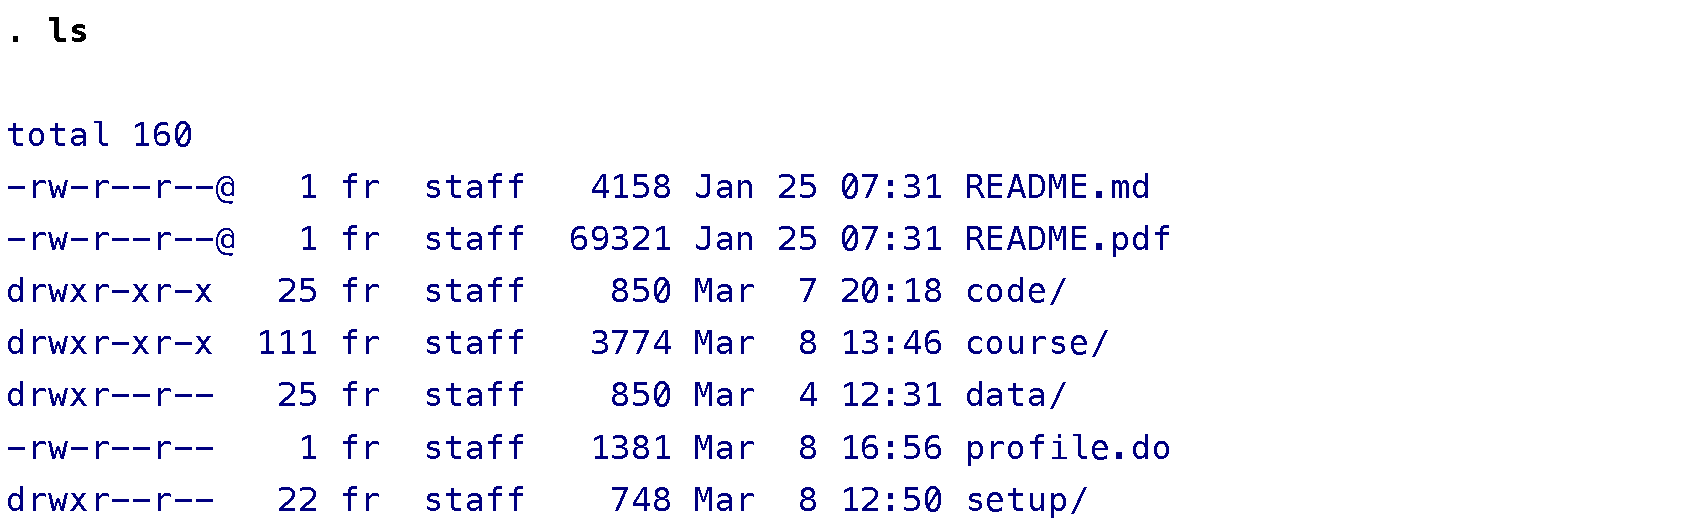
\includegraphics{srqm-ls}\\[1em]
			
	The \cmd{ls} command below will produce a more focused output by listing only the files located in the \data folder that end with the \ext{.dta} extension, which is the Stata dataset format (Figure~\ref{fig:stata-dta-icon}):%

		\begin{marginfigure}
			
\includegraphics[width=.66\textwidth]{stata-dta-icon}
			\caption{Stata~12 dataset icon.}
			\label{fig:stata-dta-icon}
		\end{marginfigure}

		\begin{docspec}
			ls data/*.dta, w
		\end{docspec}
			 
	The command will list the teaching datasets used in the course, showing only their filenames because you passed the \coab{wide}{w}{ls} option to it:\\[1em]%
 
		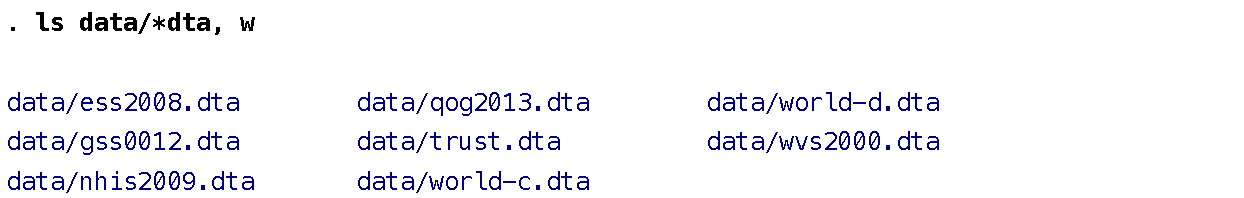
\includegraphics{srqm-ls-dta}\\[1em]
	
	To finish this little exercise with folder navigation from the command line, make sure that your working directory is the \SRQM folder. Use the \cmd{pwd} command to get the path printed once more:%
	
		\begin{docspec}
			pwd
		\end{docspec}
	
	Your working directory should again end with the \SRQM folder, which is what we need to run the course setup in the next section:\\[1em]%
	
		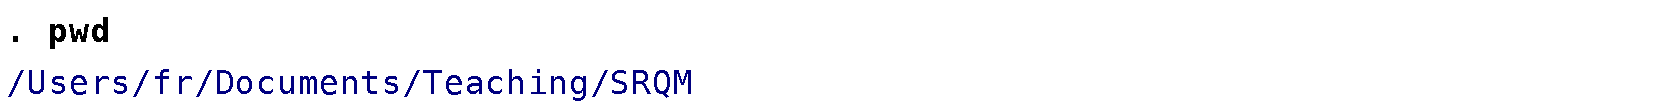
\includegraphics{srqm-pwd}\\[1em]
  
	% iii
  %
  \paragraph{Run the \SRQM setup}%
		\label{sec:setup}%

	To finish setting up your computer for the course, make sure that you are connected to the Internet, then type the following command in the Command window and press \texttt{Enter}:%
		%
		%
		
		\begin{docspec}
			run profile
		\end{docspec}
	
	\hlred{\textbf{Note:} the command will not work if you have not set the \SRQM folder as your working directory}, and that its syntax is a strict one: do not add capital letters, separate the words \texttt{run} and \texttt{profile}, and of course, use the exact spelling.%
	
	This command will trigger a bunch of setup utilities that install the additional Stata commands listed in Table~\ref{tbl:additional-commands}, uncompress the course datasets and adjust some Stata system options.%
		%
		\footnote{For example, the setup adjusts Stata memory on older versions of Stata to deal with some of the larger course datasets. Stata~12 now handles memory automatically.} %
		%
		%
		
	\bigskip

\begin{fullwidth}
	\begin{table}
		\footnotesize
		\begin{tabular}{lll}
		\toprule
		Package & Description \\
		\midrule
		\emph{Installed from the \SSC server:} & & \\
	  \quad \pkg{estout} & export regression results \\
		\quad \pkg{fre} & frequencies with value labels \\
	  \quad \pkg{kountry} & standardised regions and country names\\
	  \quad \pkg{leanout} & simplified regression results\\
		\quad \pkg{lookfor\_all} & search for variables across datasets \\
	  \quad \pkg{mkcorr} & export correlation tables\\
	  \quad \pkg{plotbeta} & regression coefficient plots \\
    % \quad \pkg{qog} & download \QOG data\\
		\quad \pkg{scheme-burd} & graph scheme \\
		\quad \pkg{spineplot} & mosaic plots \\
	  \quad \pkg{spmap} & maps \\
	  \quad \pkg{tab\_chi} & residuals for Chi-squared tests\\
	  \quad \pkg{tabout} & export summary statistics\\
	  \quad \pkg{wbopendata} & download World Bank data\\
		\addlinespace
		\emph{Installed from elsewhere:} & & \\
		\quad \label{install-gstd01}\cmd{gstd01} & standardize a variable to $0$-$1$\\%
    %; used at p.~\pageref{sec:gtsd01} \\
		\quad \label{install-clarify}\pkg{clarify} & simulation\\%
    %; used at p.~\pageref{sec:clarify} \\
    % \quad \pkg{schemes} & graph schemes \\
		\emph{Installed with the course setup:} & & \\
    % \quad \pkg{repl} & replication utility \\
		\quad \cmd{srqm} & course utilities \\
    \quad \cmd{sbar} & plots for categorical data\\
		\quad \cmd{stab} & export summary statistics tables \\
		\bottomrule%\\[1em]
		\end{tabular}
		%
		\caption{Additional commands installed by the course setup.}
		\label{tbl:additional-commands}
	\end{table}
\end{fullwidth}

%
  
	You will get a `\texttt{Hello!}' message when the setup is complete.%
	
  \hlred{\textbf{Note:} if you move or rename the \SRQM folder, the setup will break and you will have to repeat the steps covered in the previous paragraphs to fix the issue:}%
		%
		%	
		\begin{enumerate}
			\item run as administrator (if using Windows),
			\item select the \SRQM folder as the working directory, and
			\item type \texttt{run profile} to go through setup again.
		\end{enumerate}
	  
	The setup overwrites the \filename{profile.do} file of the Stata application folder to redirect it to the \SRQM folder for the time of the course. From there, it runs another \filename{profile.do} file that verifies the integrity of the teaching material and reruns parts of the setup if necessary.%
		%
		%
		
	The setup also loads the \cmd{srqm} teaching utilities, like \cmd{srqm\_get}, which is used in class to download the latest version of the course material from a temporary course server, and \cmd{stab}, which is used to produce \underline{s}imple \underline{tab}les of summary statistics (see its detailed instructions at p.~\pageref{cmd:stab}).%
    %
    %
		
  \newthought{At the end of the course}, delete the \texttt{profile.do} from the Stata application folder to stop automatically setting the \SRQM folder as your working directory. Alternately, run the \texttt{srqm\_link, clean} command to do so and get a `\texttt{Bye}' message. This will let you work with Stata from any other working directory.%
		%
		%

%
%
\subsection{Course datasets}
	\label{sec:data-sources}
	\index{Datasets!Data sources}%
	%
	%

  \newthought{Stata can load example data} with the \cmd{sysuse} and \cmd{webuse} commands, as shown with the \code{lifeexp} dataset at p.~\pageref{lifeexp}. The course provides its own teaching datasets, listed in Table~\ref{tbl:data-sources}. The course setup will also download two files to plot world maps in Stata.%

  \bigskip
\begin{table}
  \begin{center}
  \footnotesize
  \begin{tabular}{lll}
    \toprule
    Filename & Data & Year(s) \\
    \midrule
    \emph{Teaching datasets:} & & \\
      \quad \texttt{ess0810}  & \ess  & 2008--2010\\
      \quad \texttt{gss0012}  & \gss  & 2000--2012\\
      \quad \texttt{nhis2009} & \nhis & 2000--2009\\
      \quad \texttt{qog2013}  & \qog  & 2009 ± 3 years\\
      \quad \texttt{wvs2000}  & \wvs  & Wave~4, 2000\\
    \midrule
    \emph{World maps:} & & \\
      \quad \texttt{world-c} & \pkg{spmap} dataset &\\
      \quad \texttt{world-d} & \pkg{spmap} dataset &\\
    \bottomrule
  \end{tabular}
  \end{center}
  \label{tbl:data-sources}%
\end{table}


	All course datasets are in the \data folder, from where they can be loaded into memory with the \cmd{use} command. The command requires that you pass the exact file path of the dataset, and that you include quotes if the file path contains spaces. Note that the \cmd{use} command can also copy data from a \URL, which we might quickly review later on.%

  The example below will load a course dataset in memory:%

		\begin{docspec}
			* Load the National Health Interview Survey, years 2000-2009.\\
			use data/nhis9711, clear
		\end{docspec}

  Stata looks for \ext{.dta} files by default, so the file extension can be omitted from the command. The \opt{clear}{use} option ensures that Stata will load the data even if there is already modified data in memory. Because you are never going to overwrite the original datasets, you are never going to lose anything crucial by doing so.%

	Stata can only open one dataset at the time and opens data silently: if the operation succeeds, nothing is printed on screen, except for a short message if the dataset has been labelled by its creator. All datasets for this course are slightly modified versions of the original ones and will print a short message when opened:\\[1em]%
		
		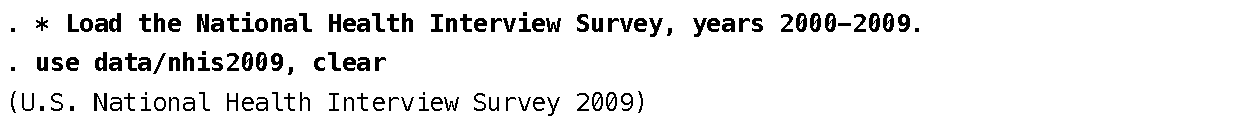
\includegraphics{use-nhis}\\[1em]%

  \newthought{The next paragraphs describe the course datasets}. These are provided in Stata 9/10 \ext{.dta} format on an ``as-is'' basis: please reference their original sources and use them for teaching purposes only. Modifications to the original files are coded in the \texttt{srqm\_data.ado} script, which is part of the course utilities.%
    \footnote{\url{https://github.com/briatte/srqm/wiki/course-utilities}}%
    
  The documentation below shows how to load the datasets in memory from the \SRQM folder with the \cmd{use} command, sometimes with an additional \cmd{if} argument to restrict the data to a particular survey year or round. Further illustrations of how to select a particular segment of your data for analysis are provided in the next sections. You will have to make your own data selection for your research project.%

\paragraph{\ess (\texttt{ess0810})}

The \texttt{ess0810} dataset holds Rounds~4~(2008) and 5~(2010) of the \ess (\ESS).%
	\footnote{\url{http://ess.nsd.uib.no/ess/round4/}}

\begin{quote}
	The \ess (the \ESS) is an academically-driven social survey designed to chart and explain the interaction between Europe's changing institutions and the attitudes, beliefs and behaviour patterns of its diverse populations.%
	\footnote{\url{http://www.europeansocialsurvey.org}}
\end{quote}

Example usage:

\begin{docspec}
  * Load the ESS dataset.\\%
  use data/ess0810, clear\\[1em]%
  %
  * Load latest survey round.\\%
	use data/ess0810 if essround == 4, clear\\[1em]%
  %
  * Load data for one country.\\%
  use data/ess0810 if cntry == "RU"\\[1em]%
  %
  * Load data for two countries.\\%
	use data/ess0810 if inlist(cntry, "CZ", "SK"), clear
\end{docspec}

The \ESS dataset should be used with the following survey weights:

\begin{docspec}
  * Set survey design weights.\\%
	svyset [pw = dweight]
\end{docspec}

See the \ESS weighting guide for details on using additional population weights to use a sample that representative of the European population.%
  \footnote{\url{http://ess.nsd.uib.no/ess/doc/weighting.pdf}} %
  You might also want to take a look at Matthias Ganniger's training module on weigthing the \ESS, which is an excellent five-chapter introduction to the topic.%
  \footnote{\url{http://essedunet.nsd.uib.no/cms/topics/weight/}}

The datasets for both rounds were downloaded from the ESS data server,%
  \footnote{\url{http://nesstar.ess.nsd.uib.no/}} %
  and the codebooks were downloaded from the \ESS data website, on which you can also find a very useful series of booklets that present overall and `topline' results.%
  \footnote{\url{http://ess.nsd.uib.no/}} %
  Check the cumulative dataset for other ESS survey waves,%
  \footnote{\url{http://ess.nsd.uib.no/downloadwizard/}} %
  and refer to the original datasets for nation-specific variables (\eg mother's education in Slovakia or party membership in Belgium).

\paragraph{\gss (\texttt{gss0012})}

The \texttt{gss0012} dataset holds data from the U.S. \gss (\GSS) for years 2000-2012.

\begin{quote}
	The \GSS contains a standard `core' of demographic, behavioral, and attitudinal questions, plus topics of special interest. Many of the core questions have remained unchanged since 1972 to facilitate time-trend studies as well as replication of earlier findings.%
	\footnote{\url{http://www3.norc.org/GSS+Website/}}
\end{quote}

Example usage:

\begin{docspec}
  * Load GSS dataset.\\%
  use data/gss0012, clear\\[1em]%
  %
  * Load latest survey year.\\%
	use data/gss0012 if year == 2012, clear
\end{docspec}

The \GSS dataset should be used with the following survey weights:

\begin{docspec}
  * Set survey design weights.\\%
	svyset vpsu [pw = wtssall], strata(vstrat)
\end{docspec}

% link to Pedlow requires fix
% http://tex.stackexchange.com/questions/12230/getting-percent-sign-into-an-url-in-a-footnote#12233

See Appendix~A of the \GSS codebook%
   \footnote{\url{http://publicdata.norc.org:41000/gss/documents//BOOK/GSS_Codebook_AppendixA.pdf}} %
   and the online technical paper ``Calculating Design-Corrected Standard Errors for the General Social Survey, 1988-2010''%
  \footnote{\url{http://publicdata.norc.org:41000/gss/documents//OTHR/GSS\%20design\%20variables.pdf}} %
   by Steven Pedlow for details, especially if you plan to use older survey years for which the sampling and weighting design are different.%

The data are extracted from the \GSS 1972-2012 cumulative cross-sectional dataset (Release 2, June 2013).%
  \footnote{\url{http://www3.norc.org/GSS+Website/Download/STATA+v8.0+Format/}}

\paragraph{\nhis (\texttt{nhis9711})}

The \texttt{nhis9711} dataset holds sample adult data for years 1997--2011 of the U.S. \nhis (\NHIS).

\begin{quote}
	The \nhis (\NHIS) has monitored the health of the nation since 1957. \NHIS data on a broad range of health topics are collected through personal household interviews. For over 50 years, the U.S. Census Bureau has been the data collection agent for the \NHIS. Survey results have been instrumental in providing data to track health status, health care access, and progress toward achieving national health objectives.%
	\footnote{\url{http://www.cdc.gov/nchs/nhis.htm}} 
\end{quote}

Example usage:

\begin{docspec}
  * Load NHIS dataset.\\%
  use data/nhis9711, clear\\[1em]%
  %
  * Load latest survey year.\\%
	use data/nhis9711 if year == 2011, clear
\end{docspec}

The \NHIS dataset should be used with the following survey weights:

\begin{docspec}
    * Set survey design weights\\
    svyset psu [pw = perweight], strata(strata)
\end{docspec}

See the IHIS/NHIS user notes on variance estimation for more details.%
  \footnote{\url{http://www.ihis.us/ihis/userNotes_variance.shtml}}

The data come from the Integrated Health Interview Series website.%
  \footnote{\url{http://www.ihis.us/}} %
  In the course, we use this dataset to illustrate normality in the distribution of the Body Mass Index in American adults. Our class estimates will slightly differ from the official figures because we will be using the public \nhis files, in which extreme observations of height and weight have been redacted. The data contain an additional variable for race and ethnicity, based on a simplified version of the official classification standard.%
  \footnote{\url{http://www.whitehouse.gov/omb/fedreg_race-ethnicity}}%

\paragraph{\qog (\texttt{qog2013})}

The \texttt{qog2013} dataset holds the \qog (\QOG) Standard cross-sectional dataset in its most recent revision of May~15, 2013. The data are country-level aggregates centered around 2009 $\pm$ 3 years.%

\begin{quote}
	Our research addresses the questions of how to create and maintain high quality government institutions and how the quality of such institutions influences public policy in a broader sense.%
  \footnote{\url{http://www.qog.pol.gu.se/}}%
\end{quote}

Example usage:

\begin{docspec}
  * Load QOG dataset.\\%
  use data/qog2013, clear%
\end{docspec}

The data and codebook come from the \QOG Standard download page.%
   \footnote{\url{http://www.qog.pol.gu.se/data/qogstandarddataset/}}

\paragraph{\wvs (\texttt{wvs2000})}

The \texttt{wvs2000} dataset holds data from Wave~4 (1999-2004) of the \wvs (\WVS).

\begin{quote}
	The \wvs (\WVS) is a worldwide network of social scientists studying changing values and their impact on social and political life. The \WVS in collaboration with EVS (European Values Study) carried out representative national surveys in 97 societies containing almost 90 percent of the world's population. These surveys show pervasive changes in what people want out of life and what they believe. In order to monitor these changes, the EVS/WVS has executed five waves of surveys, from 1981 to 2007.%
	\footnote{\url{http://www.worldvaluessurvey.org/}}
\end{quote}

Example usage:

\begin{docspec}
  * Load WVS dataset.\\%
  use data/wvs2000, clear\\[1em]%
  %
  * Load data for one country (using numeric code).\\%
	use data/wvs2000 if v2 == 4, clear\\[1em]%
  %
  * Load data for two countries (using names).\\%
  use data/wvs2000, clear\\%
  decode v2, gen(country)\\%
  keep if inlist(country, "Iran", "Iraq")\\%
  drop v2%
\end{docspec}

The \WVS dataset should be used with the following survey weights:

\begin{docspec}
  * Set survey design weights.
	svyset [pw = s017]
\end{docspec}

See the \WVS weighting guide for details.%
  \footnote{\url{http://www.jdsurvey.net/jds/jdsurveyActualidad.jsp?Idioma=I&SeccionTexto=0405}}

The data come from the official file found at the \WVS website.%
   \footnote{\url{http://www.wvsevsdb.com/}} %
   This version has encoding issues that are used as examples to teach recoding. The cumulative dataset has different variable names and proper variable encoding. More recent data is also currently getting assembled in Wave~6 (2010-2013) of the \wvs.%
  \footnote{\url{http://www.wvs-online.com/}}
%
%

\stopcontents[chapters]

%
% have a nice day
%
         %% ... session 1 (course, toc)
	
  % 1) data viz
  % 
  %
% 2
%
\chapter{Datasets}%
	%
	\label{ch:data}%
	\index{Datasets}%
	%
  \begin{mybox}
    %
    \smallcaps{This section} deals with data management. Because we will be using course datasets and preinstalled Stata commands, you will need to have \textbf{run the course setup} as explained in Section~\ref{sec:course-setup} to follow from here on.%
    %
    \paragraph{Coursework} %
    This section is covered in class during Weeks~2--3. Make sure that you have fully replicated the course do-files for these weeks by the end of this section. Read \citeauthor[ch.~2--3]{Urdan:2010a}, and optionally \citeauthor[ch.~2.1--2.4]{FeinsteinThomas:2002d}.%
    %
  \end{mybox}\\[4em]%
  %
  \startcontents[chapters]%
  \printcontents[chapters]{l}{1}{\setcounter{tocdepth}{2}}%
	%
	\newpage
	%

% 0. intro (use, count, use if)

\newthought{Quantitative data} is a form of data that simplifies information into variables that take different types and values. Some variables, such as gross domestic product or monthly income, hold \emph{continuous} data that are strictly numeric, while others hold \emph{categorical} data, such as social class for individuals or political regime type for nation states.%

As in qualitative research, the collection of data for quantitative analysis systematically raises issues of conceptualisation, measurement and reliability, with specific issues related to the sampling design that makes a sample representative of a target population, like the residents of a country.%

\newthought{Manipulating a dataset} is itself a complex task that requires some familiarity with the structure of the data, with the software commands available to prepare the data, and with the research design of your project. Using predefined datasets, as we will in this course, will simplify these operations a great deal, but will not entirely suppress them, so that we can learn some of the basics of data management and preparation.%

This section describes the essential steps that you should follow to prepare your data before starting your analysis. It also outlines some complementary data skills that will serve you if you have to work with quantitative data beyond the scope of this course.%

\newthought{A dataset} is a file that contains a set of variables for a given number of \emph{observations}. Each row of the dataset holds a single observation, and each column holds a single variable. The data will usually start with an `ID' or `Name' variable, which might be the country name or code in a country-level dataset, or a unique identifier code in an anonymous individual-level survey. That variable is set to characterise each \emph{unit of analysis} of the data, which might be just anything: countries, firms, NGOs, individuals, historical events, etc.%

% \input{T_data_cs}

\bigskip
\begin{table}
\begin{center}
\footnotesize
\begin{tabular}{lllll}
\toprule
Observation & ID & Variable 1 & Variable 2 & ... \\
\midrule
\emph{Country-level data:} & & & & \\
\quad 1. & Afghanistan   & Value   & Value   & ... \\
\quad 2. & Albania & Value & \na & ... \\
\quad 3. & Algeria   & Value   & Value   & ... \\
\quad ... & & & & \\
\addlinespace
\emph{Individual-level data:} & & & & \\
\quad 1. & 17534   & Value   & Value   & ... \\
\quad 2. & 17535 & Value & Value & ... \\
\quad 3. & 17536   & \na   & Value   & ... \\
\quad ... & & & & \\
\bottomrule
\end{tabular}
\caption{Basic data structures, with observations in rows and variables in columns. Note that the variables have some missing values.}
\label{tbl:basic-data}
\end{center}
\end{table}

\bigskip
\newthought{The total number of observations} of a dataset is denoted $N$. It might be small, as with $N = 27$ OECD countries, or huge, as with `big data' where $N > 100,000$. Statistical tests can easily fail to apply when the number of observations is low, typically somewhere around $N < 30$. The data can also suffer from overall sparsity if there are few variables or many missing values. 

Basic data structures like those shown in Table~\ref{tbl:basic-data} are \emph{cross-sectional} because they contain data for only one time period. Datasets that contain values for more than one time period $T$ are called \emph{time series}. Table~\ref{tbl:csts-data} shows an example of cross-sectional time series.

% \input{T_data_csts}

\bigskip
\begin{table}
\begin{center}
\footnotesize
\begin{tabular}{lllll}
\toprule
Observation & ID & Year & Variable 1 & ... \\
\midrule
\quad 1. & France & 2010 & Value & ... \\
\quad 2. & France & 2011 & Value & ... \\
\quad 3. & France & 2012 & Value & ... \\
\quad 4. & Germany & 2010 & Value & ... \\
\quad 5. & Germany & 2011 & \na & ... \\
\quad 6. & Germany & 2012 & Value & ... \\
\quad ... & & & & \\
\bottomrule
\end{tabular}
\caption{Cross-sectional time series, a.k.a. \smallcaps{csts} data. This data structure is common in some research areas like international relations and comparative politics. In a dataset that counts $N = 27$ countries over $T = 20$ years, the total number of country-year observations will be $27 \times 20 = 540$, or less as soon as there are missing values.}
\end{center}
\label{tbl:csts-data}
\end{table}

\bigskip
The structure of the data can get even more complex if there is more than one \emph{level of observation} nested within each other, as when some respondents are taken from the same household, region and country. Furthermore, the observations can repeat over time and form a \emph{panel}, as when epidemiologists observe a cohort of adults through their life course in a longitudinal study. Table~\ref{tbl:panel-data} shows an example of cross-country household panel data.

% \inpit{T_data_longit}

\bigskip
\begin{table}
\begin{center}
\footnotesize
\begin{tabular}{lllllll}
\toprule
Observation & Country & Year & Household ID & Person ID & Variable 1 & ... \\
\midrule
\quad 1. & Turkey & 2011 & 907 & 24101 & Value & ... \\
\quad 2. & Turkey & 2012 & 907 & 24102 & Value & ... \\
\quad 3. & Turkey & 2011 & 908 & 24103 & Value & ... \\
\quad 4. & Turkey & 2012 & 908 & 24104 & Value & ... \\
\quad 5. & Ukraine & 2011 & 403 & 46889 & Value & ... \\
\quad 6. & Ukraine & 2012 & 403 & 46890 & Value & ... \\
\quad 7. & Ukraine & 2011 & 404 & 46891 & \na & ... \\
\quad 8. & Ukraine & 2012 & 404 & 46892 & \na & ... \\
\quad ... & & & & & & \\
\bottomrule
\end{tabular}
\caption{Panel data, with individuals nested in households nested into countries. The time period covered by panel data can range from a few years for repeated surveys to decades for longitudinal studies of patient cohorts in biomedicine or financial time series holding stock values.}
\end{center}
\label{tbl:panel-data}
\end{table}

\newthought{In this course}, we focus on cross-sectional data in which we can assume that the observations are independent from each other. Special methodological requirements apply to panel data and times series, where this requirement is violated by the temporal dependence between recurring observations.\footcite{BeckKatz:2011e}%

A selection of datasets is available from the \data folder. It contains three individual-level surveys using large probability samples: the \ess (\ESS), \gss (\GSS) and \wvs (\WVS). For country-level analysis, the recommended source is the \qog (\QOG) Standard Dataset, which collates together variables from the World Bank and the United Nations as well as academic research and various other sources. All datasets are high quality sources.%

\newthought{For your project}, select one of these datasets and fetch additional documentation from the course appendix at p.~\pageref{sec:data-sources}. You will need to get the data codebook as well as information on the \emph{sampling procedure} if you are using survey data. The sampling procedure is the technique that guarantees the representativeness of the sample by ensuring that each member of the target population had an equal probability of selection within the sampling frame.%

Several techniques can enhance simple random sampling procedures, such as stratified or cluster sampling, where primary sampling units (\eg individuals) are selected within nested structures (\eg households). Weighting schemes can also provide postsurvey adjustment to correct for undercoverage, \ie the existence of different probabilities of selection among the survey respondents. You will find mentions to survey weights in the codebooks of your dataset and in the data appendix, so that you can easily set them in your own analysis.%

\label{external-data-warning}%
\newthought{Using external data sources for your research project}%
	\footnote{See the course wiki for a short selection: \url{https://github.com/briatte/srqm/wiki/data}} %
  is \textbf{not} recommended for this course, due to the extra workload that it will inflict on your group at the data preparation level. If you plan to ask for an exception, please make that decision reasonably and plan your work well in advance, especially if you have not yet assembled the data, which is an \emph{extremely} time-consuming task. \hlred{You will be asked to abandon any effort that has not been successful in the first month of class.}%
		%

You need to read this section to achieve three goals:

\begin{enumerate}
	\item \textbf{Prepare your dataset for analysis.} The code for this operation will form the first segment of your do-file, in which you check the description and encoding of your variables, and possibly recode some of them.
	\item \textbf{Describe the variables.} You will be required to provide summary statistics for continuous variables and relative frequencies (percentages) for categorical ones. More on variable types in a few pages.
	\item \textbf{Preserve a high sample size.} Your data preparation code will end on a diagnosis of how missing values affect your sample, as you will be required to delete all observations that contain missing values.
\end{enumerate}
   
Next to the data itself, you should now also organize and open the data documentation to read about the variables that you will be preparing for analysis.%

%
%
% 1
%
\section{Essential data skills}

	%
	%
  \newthought{This section shows how to manipulate datasets.} Start by opening the \ess:\\[1em]

		\begin{docspec}
			* Load the \ess, Rounds 4 (2008).\\
			use data/ess2008 if essround == 4 \& cntry == "FR", clear
    \end{docspec}
    
		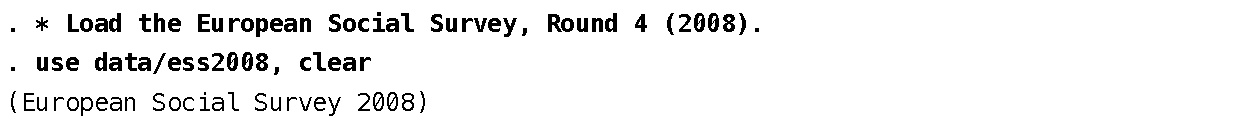
\includegraphics{use-ess}

  Notice that we are limiting the observations to a single country in a single survey round, as to get some data in the most basic cross-sectional structure. Similarly, when we use the \nhis, we limit the data to one year of data:%
  
    \begin{docspec}
      * Load the \nhis, latest survey year.
      use data/nhis9711 if year == 2011
    \end{docspec}
    
  You can build small-scale comparisons through time and space, \eg by comparing respondents from 2002 with respondents from 2012 in the \gss:%
  
    \begin{docspec}
      * Load the \gss, selected years.
      use data/gss0012 if inlist(year, 2002, 2012)
    \end{docspec}
    
  If you want to compare across countries from the \wvs or from the \ess, select a small number of cases out of the country code variables (consider three an operational maximum):%
  
    \begin{docspec}
      * Load data for one country (using numeric code).\\%
    	use data/wvs2000 if v2 == 4, clear\\[1em]%
      %
      * Load data for two countries (using names).\\%
      use data/wvs2000, clear\\%
      decode v2, gen(country)\\%
      keep if inlist(country, "Iran", "Iraq")\\%
      drop v2%
    \end{docspec}
    
	%
	%
	\newthought{Now take a look at the data.} Use the \cmd{browse} command to inspect the dataset in the Data Editor, which gives you a raw feel of the data in the `editor' layout that you know from spreadsheet editors:%

		\begin{docspec}
			browse
		\end{docspec}

  Optionally, you could have added a selection of variables to the \cmd{browse} command in order to show only some columns of the dataset:\\[1em]%

		\begin{docspec}
			use data/qog2013, clear\\
			browse ccode-version
      browse cname unna\_pop
		\end{docspec}

	The \cmd{browse} command is an exploratory command: it is a convenience tool to look at the data in read-only mode. You do not need to write exploratory commands like \cmd{browse} to your do-file, they are only meant to help you visualize the raw data.%
  	
  You should now be looking at the `top-left' observations and variables of the \QOG dataset, where you can see some unique identifier variables, like the version number of a dataset or the numeric codes and names of the country observations (Figure~\ref{fig:qog-browse}).%

		\begin{figure*}[h]
			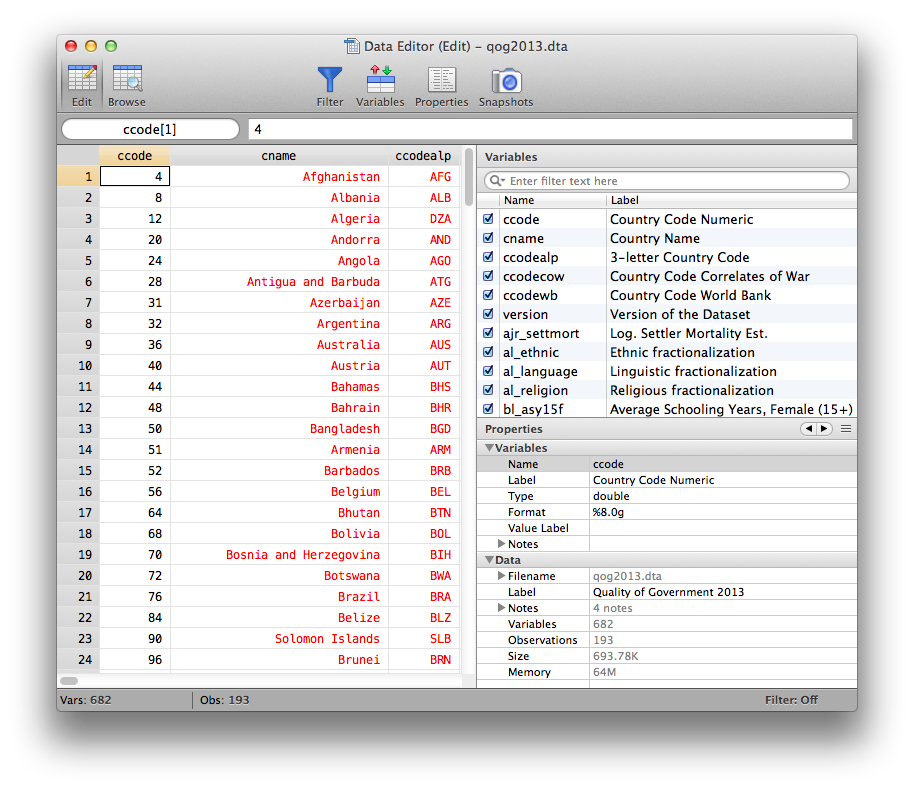
\includegraphics{qog-browse-screenshot}%
		  \caption{The Stata Data Browser, showing \QOG data.}%
		  \label{fig:qog-browse}%
		\end{figure*}

	%
	%
	Notice the different variable colors used in the Data Browser: in Figure~\ref{fig:qog-browse}, numeric measures are shown in black, whereas text descriptions, called `strings' in computer environments, are shown in red. While numeric values can be referred to directly in computing environments, strings require to be enclosed in \texttt{"quotes"} to be recognized as such.%
		
	There is another kind of variable \emph{encoding} that combines numeric values and text labels by assigning numbers to categories, groups or response items, like 1 coding for `Strongly agree' and 5 for `Strongly disagree'. These variables are shown in blue in the Data Browser, as illustrated with the \gss:\\[1em]%

		%
		\begin{figure*}[h]
			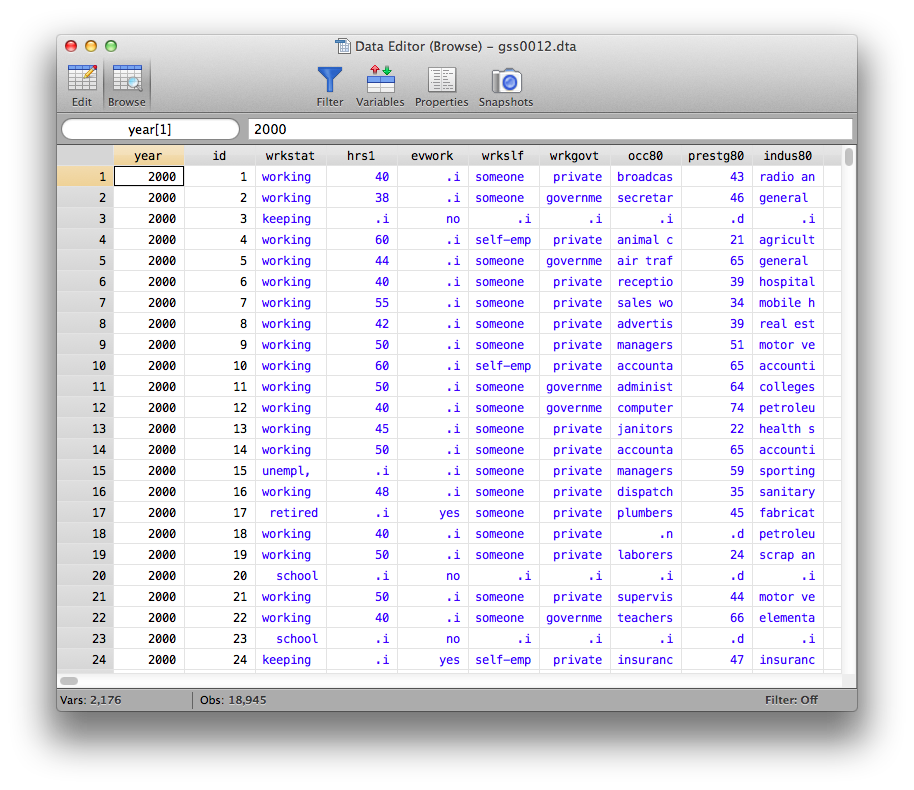
\includegraphics{gss-browse-screenshot}%
		  \caption{The Data Editor in Browse (read-only) mode, showing \GSS data.}%
		  \label{fig:gss-browse}%
		\end{figure*}

	In Figure~\ref{fig:gss-browse}, the blue color indicates that, for the \texttt{wrkstat} variable of the \gss, there is both a numeric coding scheme of the type 1, 2, etc., and a set of labels that correspond to employment categories: 1 for `Working full-time', 2 for `Working part-time', etc.%

	In Figures~\ref{fig:qog-browse} and \ref{fig:gss-browse}, some observations (rows of data) show values that start with a full period (\texttt{.}). This is how Stata codes \emph{missing values}. This scheme is idiosyncratic to Stata, and missing values can be coded differently (\eg by \texttt{NA}, \texttt{-1} or \texttt{999}) depending on the data collection protocol.%

	%
	%
	\newthought{Let's take a closer look at the values} by producing quick data extracts from a few variables and observations. We are going to use the \cmd[li]{list} command with the \cmd{li}{list} command followed by a few variable names and row numbers, from 1 to \texttt{\_N} where \texttt{\_N} is the total number of observations that you can get with the \cmd{count} command:%

		\begin{docspec}
			* Load Quality of Government data (2013).\\
			use data/qog2013, clear\\[1em]
	
			* Ask for the total number of observations.\\
			count\\[1em]
	
			* Alternately, ask for the "raw" result.\\
			di \_N
		\end{docspec}

		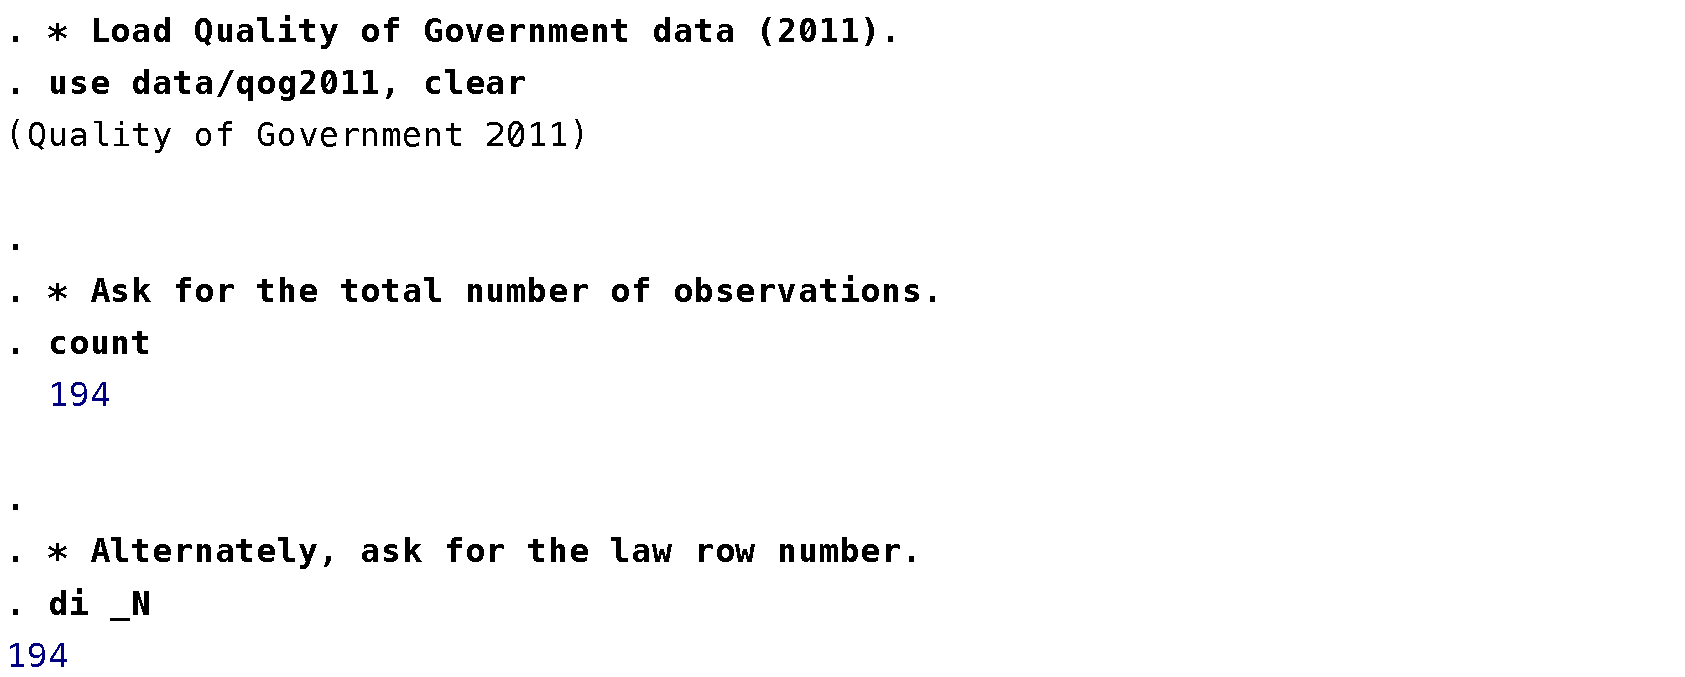
\includegraphics{qog-use-count}\\[1em]

  %%%

  \hlred{\textbf{Important:}} given its country-level unit of analysis, the \QOG dataset runs a smaller number of observations than the other teaching datasets used in the course. The largest possible sample of these countries is necessary to work with this dataset.%

  Thus, if you are using country-level data, do \emph{not} attempt to subset the \qog dataset to a particular selection of countries. The sample size is already very low in a country-level cross-section, as there are just that many countries at a given point in time.%
  
  If you still wish to take geographical context into account in your analysis, use the \cmd{kountry}\pkgfirst{kountry} package as described at p.~\pageref{qog:geo} to add regional descriptors to the \qog dataset, and compare across all available regions.%

  %%%
  
  \hlred{\textbf{Important:}} like the \cmd{browse} command, the \cmd[li]{list} command is just a convenience tool to take a look at the raw data. Listing the data is done only for exploratory motives: do not publish raw data listings or even save them to your log.%
  
  Similarly, when you are writing your analysis to a do-file, you do not need to make your code list the variables or the observations: describe only the parts of the data that are specifically relevant to your research, such as the names and labels of your selected variables.%

  %%%
  
  Let's use the \cmd{browse} command to read a few variables by passing their names to the \cmd{browse} command:%
		%
		\begin{docspec}
			browse cname-version\\
		\end{docspec}

%%%%%%%%%%fix!

\begin{docspec}
	* List first ten observations.\\
	li cname ccodealp in 1/10, clean\\[1em]
	
	* List last ten observations.\\
	li cname ccodealp in -10/l, clean
\end{docspec}

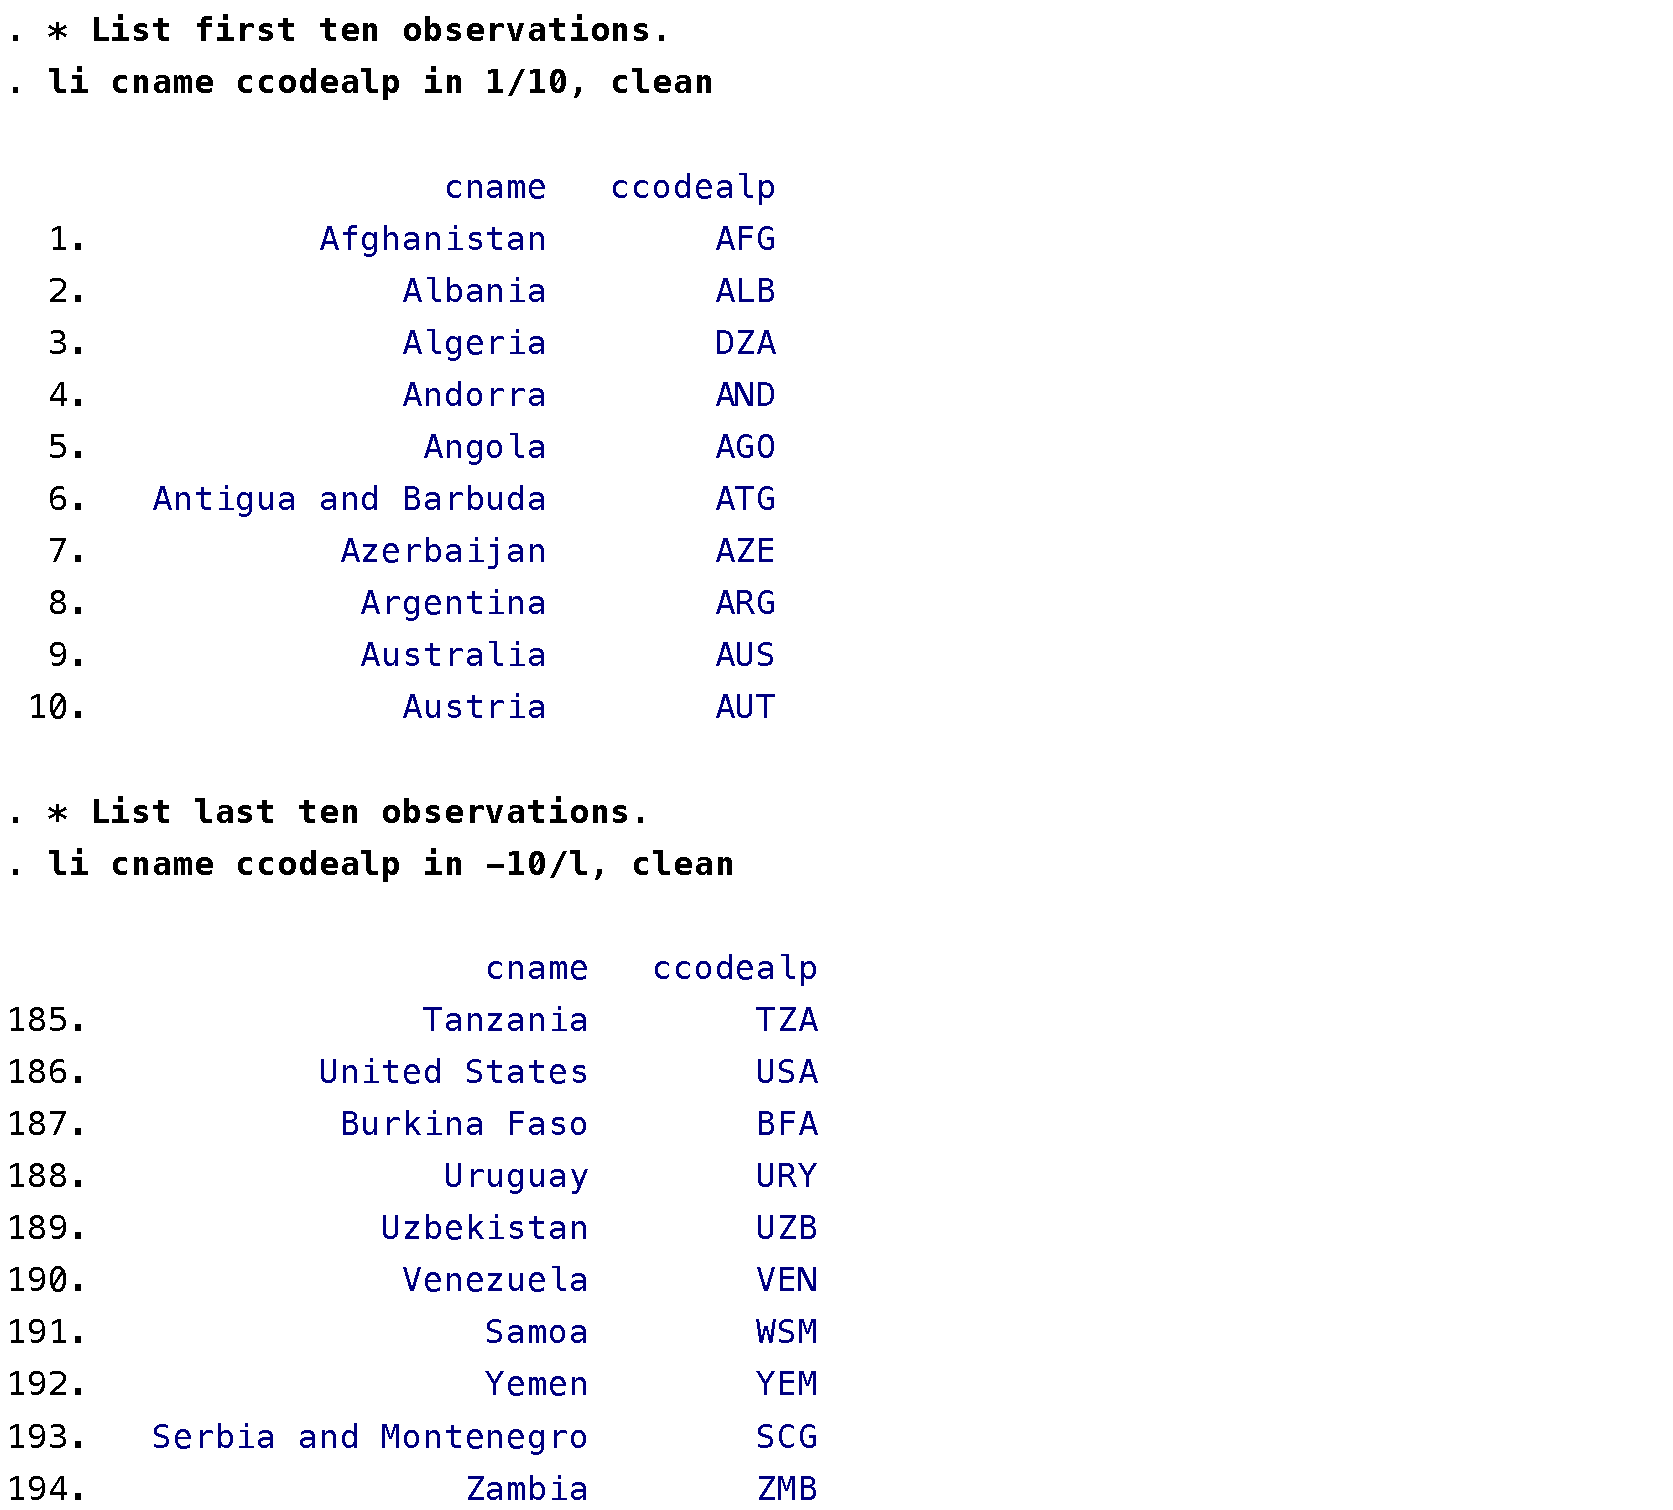
\includegraphics{qog-li-cname-ccodealp}\\[1em]

The \cmd{in} operator selects observations by their row number, which has limited use in most circumstances.%
	\index{Selectors!Observation ranges: \cmd{in}} %
	What you usually want to do instead is to select observations according to a given condition, which we will see how to do very soon.

\newthought{Describe the variables.} The command to list all variables in a dataset is \cmd[d]{describe}, which is more or less the first command that you want to run right after opening a dataset, if only to verify that the data have loaded properly. It can be used on its own or provided with a list of selected variable names:\\[1em]

\begin{docspec}
	use data/ess2008, clear\\
	d agea gndr edulvla
\end{docspec}

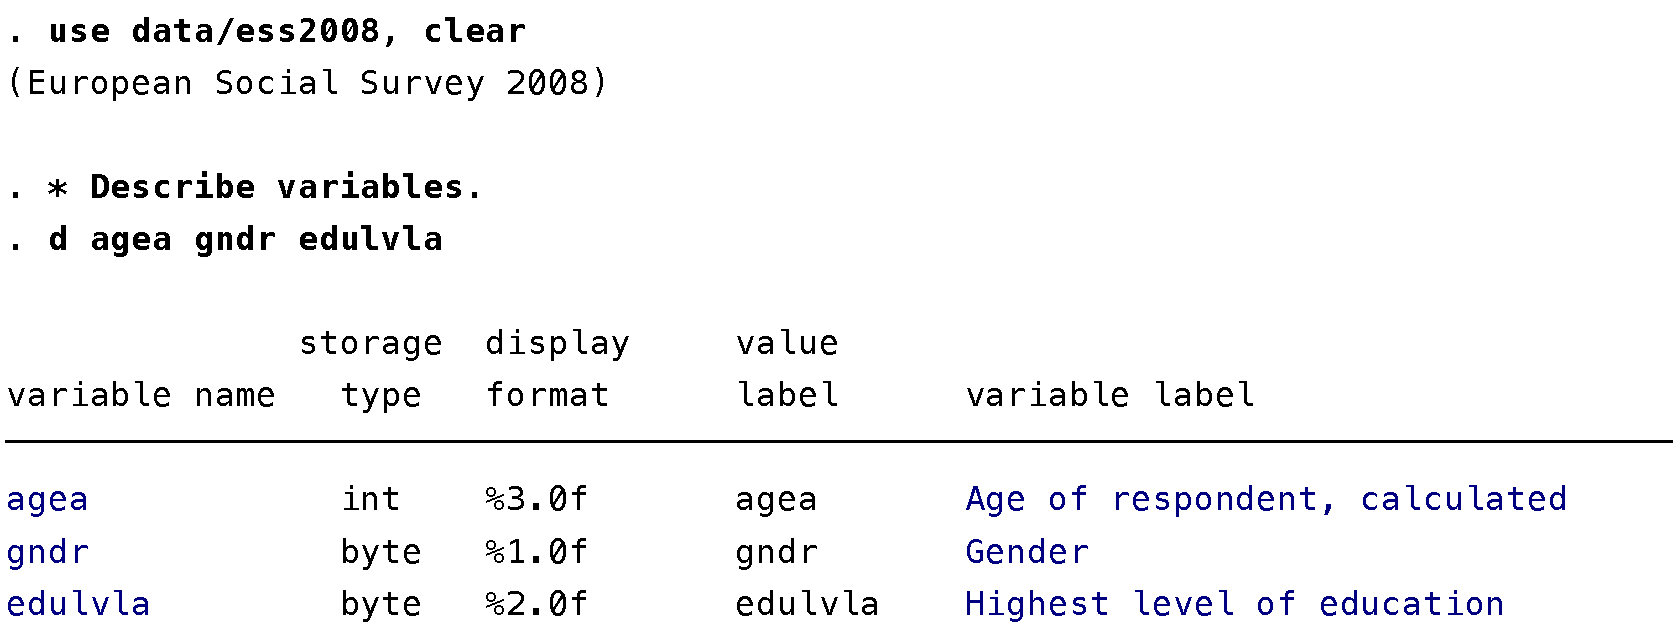
\includegraphics{ess-d}\\[1em]

To find variables by name or keyword, use the \cmd{lookfor} command:\footnote{You can also use the wonderful \cmd{lookfor\_all} command to search across datasets. Once installed by the course setup, the command allows you to search all datasets in the \data folder, as in this example with the \texttt{health} keyword:%
		%
		\begin{docspec}
			lookfor\_all health, dir(data)
		\end{docspec}}\\[1em]

\begin{docspec}
	use data/gss0012, clear\\
	lookfor homosex army
\end{docspec}

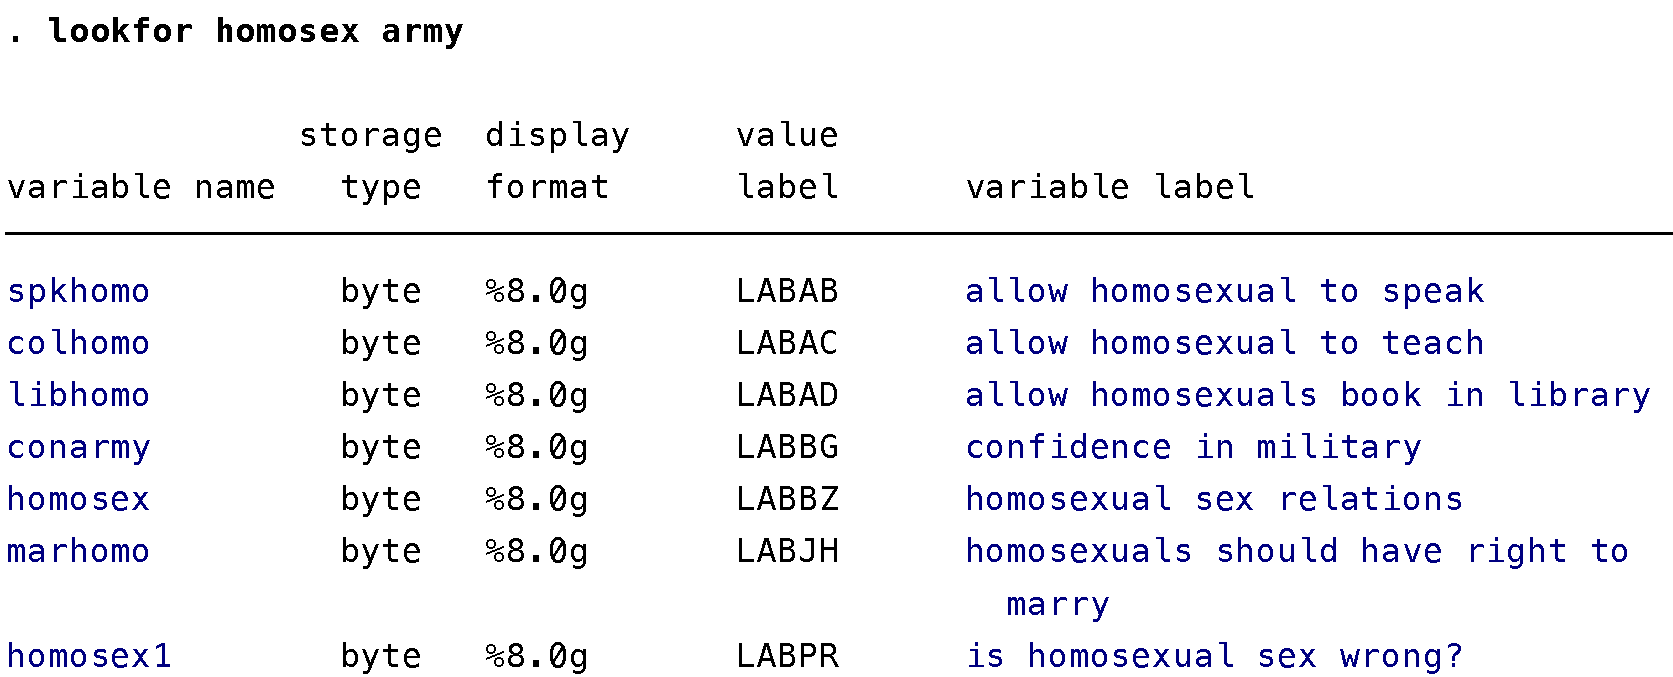
\includegraphics{gss-lookfor-homosex-army}\\[1em]

At that stage, in the best of cases, your variables of interest are ready for use, being present in the dataset in the format and with the descriptors that you want. An example would be this short selection of variables from the \QOG dataset:

	\begin{docspec}
		use data/qog2013, clear\\
		d cname ccodealp wdi\_fr wdi\_gdpc
	\end{docspec}
	
	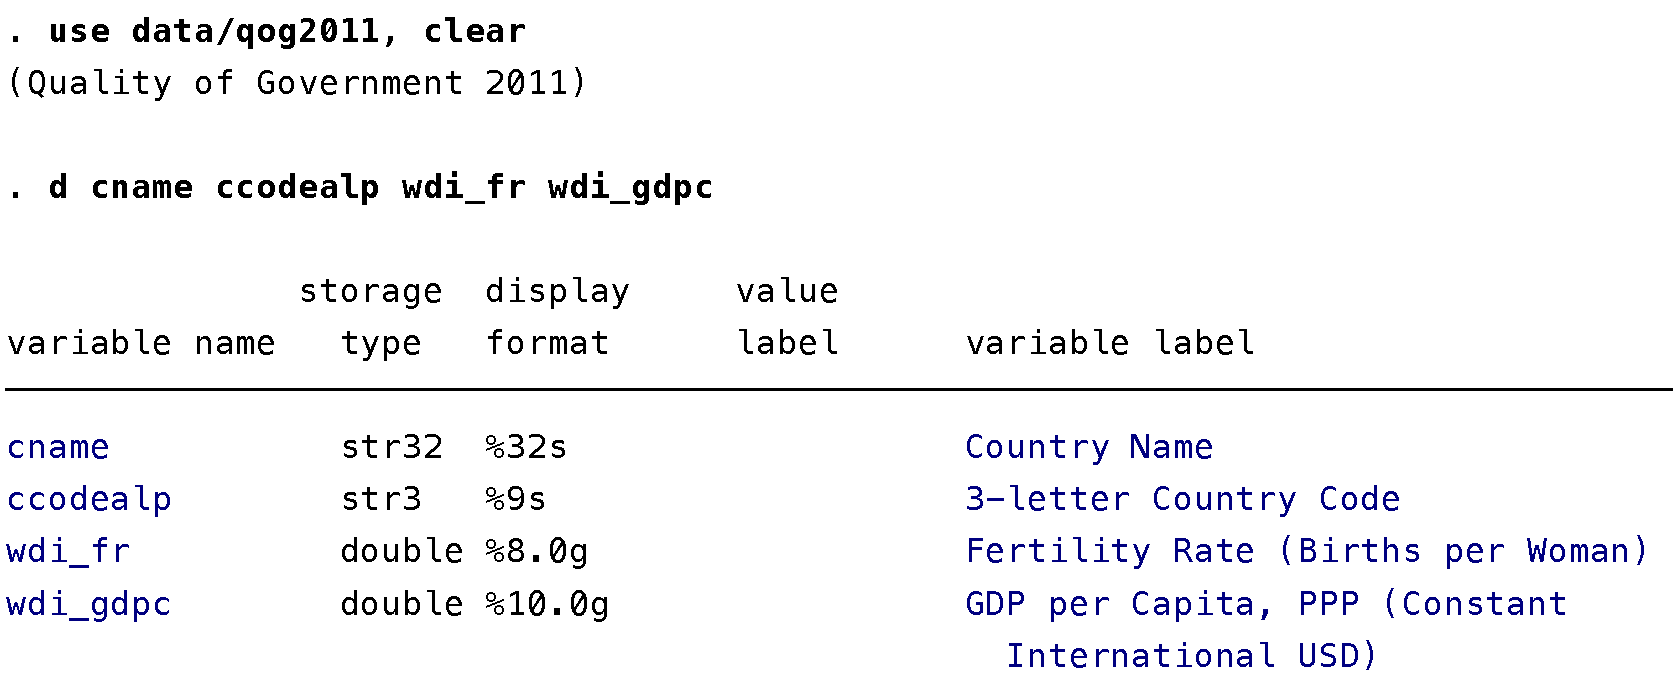
\includegraphics{qog-d}

Just two things might need a bit of adjustment at that stage. First, you might want to change the \emph{variable names} to more familiar ones by using the \cmd[ren]{rename} command. The command requires old and new variable names, and can work on many variables at the same time.%

For example, in the \qog dataset, you might want to pick your own name for the country name variable, which is often used during analysis:%

	\begin{docspec}
    * Rename country name variable.
    ren cname country
  \end{docspec}

  The \cmd[ren]{rename} command succeeds silently, with no output:

  %%fix: update
	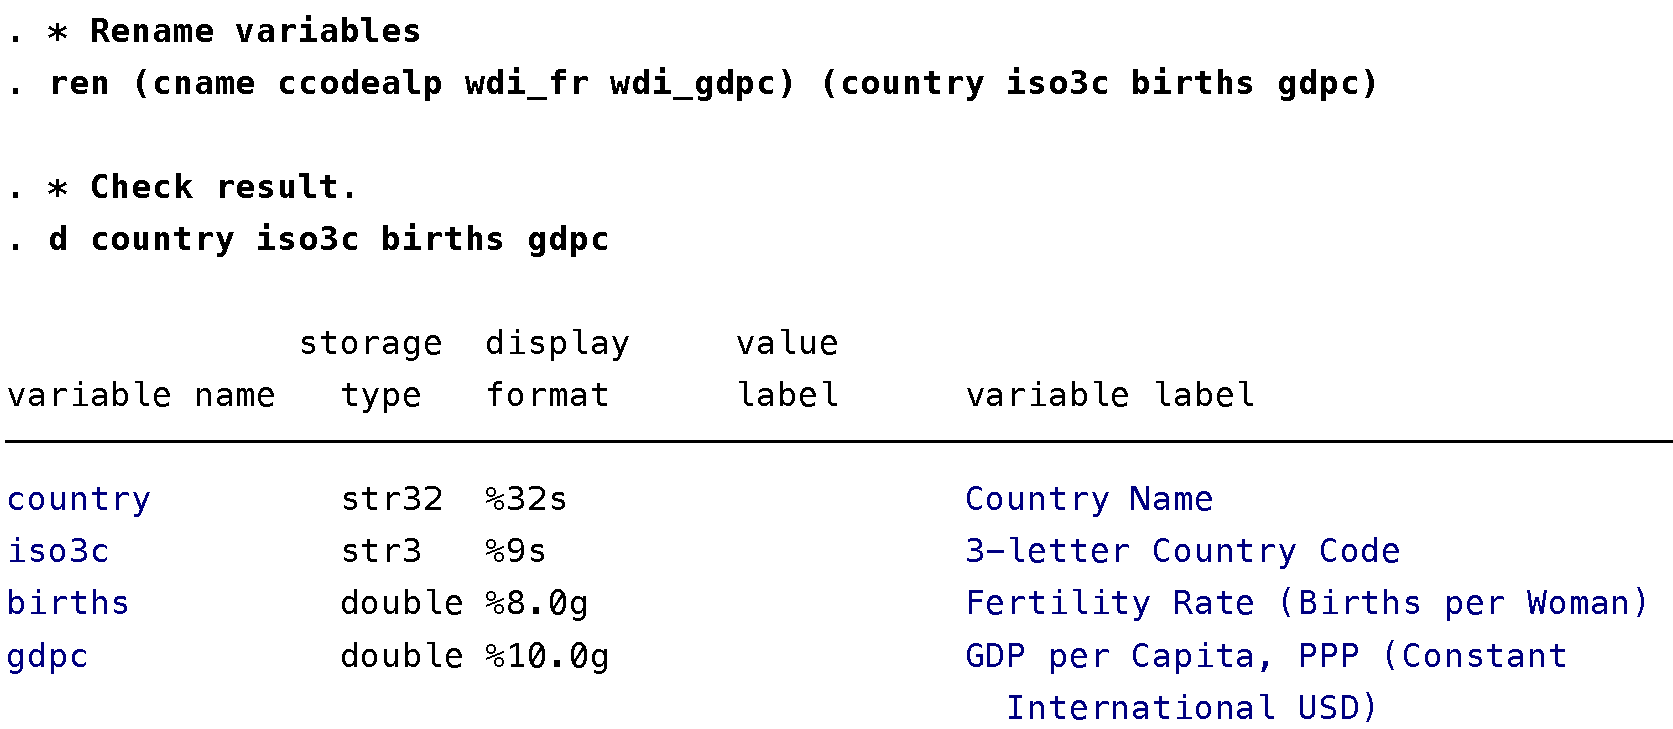
\includegraphics{qog-ren}

\label{qog:geo}%
Similarly, if you are interested in countries from a specific geographic region, you can obtain a simple continental from the \cmd{kountry} package, which creates a variable called \texttt{GEO} holding five UN~Stats standard regions.%
  \footnote{The \qog dataset includes the \texttt{ht\_region} variable holding ten regions.} %
  For consistency, we will rename the variable to lowercase:%

  	\begin{docspec}
      kountry ccode, from(iso3n) geo(un)\\
      ren GEO geo
    \end{docspec}

% Note: this variable can later be used to measure regional specificities, but it does \emph{not} come with an intrinsic reason for inclusion into your research design: it is still left to you to support the hypothesis of meaningful geographical effects in your data.%
  
You might also want to use the \cmd{renvars} \pkgfirst{renvars} command to batch rename variables (which is something that Stata~12 also knows how to do, with more code). Use a backslash to separate the list of old and new variable names:%

	\begin{docspec}
    * Rename two WDI indicators.
    renvars wdi\_fr wdi\_gdpc \textbackslash{} births gdpc
		* Check result.\\
		d country births gdpc
	\end{docspec}

\index{Variables!Labels}\index{Labels!For variables}%
Then, you might also want to adjust \emph{variable labels}, which are the short pieces of text attached to each variable. Use the \cmd[la var]{label variable} command to change the variable label to something meaningful, \eg mentioning the unit of measurement of the variable.%

\begin{mybox}
  \paragraph{Example: political positioning (\ESS)}%
    \label{ess:lrscale}%
  %
  The \texttt{lrscale} variable of the \ess is an 11-point self-placement scale measure of political position, from left-wing (\texttt{0}) to right-wing (\texttt{10}):%
  
	\begin{docspec}
		use data/ess0810, clear\\
    codebook lrscale, c
  \end{docspec}

  To remember that coding, we can rename the variable to the mnemonic \texttt{rightwing}, as to imply that the higher the value of the variable is, the more right-wing the respondent declared to be:%
  
	\begin{docspec}  
		ren lrscale rightwing
		la var rightwing "Left-wing to right-wing (0-10)"\\
  \end{docspec}

  The label makes certain that the coding will be unambiguous to the reader in the future. Relabelling the variable to indicate how the measure is to be interpreted is also useful to later include the variable in a descriptive table.%
  
	\begin{docspec}
    d rightwing
	\end{docspec}

\end{mybox}

It is generally a good idea to have variable labels that will provide something informative to graphs where they appear as axis titles. Short titles with some indication of the underlying coding scheme usually do the trick.

One last aspect of data preparation that might be of some use is to subset (\ie to restrict) the dataset to the variables that you are going to use. To do so, pass the names of your variables to the \cmd{keep} option, as in \statacode{keep v1 v2 v3} etc. I however strongly suspect this requirement to be some form of older computing age legacy that would now apply only in only few cases of large data and small memory, so I recommend \emph{not} doing this by default.

\newthought{Essential data skills} include being able to further distinguish between types of variables (p.~\pageref{sec:variable-types}), to encode missing values so that the software recognizes them (p.~\pageref{sec:missing-values}), and to recode variables to alternative groups and categories (p.~\pageref{sec:categorical-recodes}).

These skills are explained below, along additional skills that will be useful to those working with external data sources, and more advanced skills for more complex research projects.%

%
% 1.1
%
\subsection{Variable types}
\label{sec:variable-types}

You will usually want to know two things about all your variables:

\begin{enumerate}
	\item What is the \textbf{unit of measurement} of the variable? Is it meaningful, or are the numbers just a convenient to order or code some category?
	
Note in passing that what you see in a dataset is the endpoint of a social activity, and that data of all sorts are hardly neutral assets. Quantification and commensuration are conflictual process that can have critical policy implications, especially in the case of rankings and benchmark indicators of public and private performance.%\cite{EspelandStevens:2009n,Briatte:2012a,DavisFisher:2012x}

	\item What is the \textbf{coding scheme} to read the values? Is the variable made of strictly text, strictly numbers, or does it use both jointly?
\end{enumerate}

Variables can be classified into a certain number of types from these criteria: if the unit of measurement includes a true zero, if the measures can be meaningfully ordered, whether they are equally intervalled, …

But then, you probably want to learn only about the three practical categories to which all variables types eventually boil down when it is time to actually get to manipulate the data:

\begin{enumerate}
	\item \textbf{Continuous variables} like age, income, GDP per capita, male-to-female income ratio, percentage of people below the poverty line…
	\item \textbf{Categorical variables} like age and race \emph{groups}, income \emph{deciles} or \emph{bands}, marital status, 5-point agreement scales…
	\item \textbf{Dummy variables} (`dummies') that take only 0 and 1 values to code for a TRUE/FALSE statement like `is married' or `is a democracy'.
\end{enumerate}

\begin{description}
	\index{Variables!Continuous variables}%
	\item[Continuous variables] have meaningful units and generally high dimensionality: they take many different numeric values that require a unit of measurement, like years or constant dollars, to be interpreted. The average value of a continuous variable can be meaningfully interpreted: `the average fertility rate' is meaningful to some extent, while `the average race' is meaningless.

	Continuous variables are called `continuous' because their values can be any number in a given segment of the real number line $\mathcal{R}$. For many variables like age or GDP growth, there is an infinity of values: your exact age can be any positive number $(26, 26.1, 26.01, ...)$, and GDP growth theoretically ranges from negative to positive infinity. The effective number of values taken by a continuous variable is limited by measurement precision and by the empirical range of the variable: age, for instance, is usually a variable composed of around 100 possible values expressed in years.

	The example below shows the output of the \cmd{codebook} command for a continuous variable from the \qog dataset. The \texttt{wdi\_gdpc} variable measuring GDP per capita takes 178 unique values, ranging from 226 to over 63,000 constant international dollars:\\[1em]
	
	\begin{docspec}
		use data/qog2011, clear\\
		codebook wdi\_gdpc
	\end{docspec}
	
	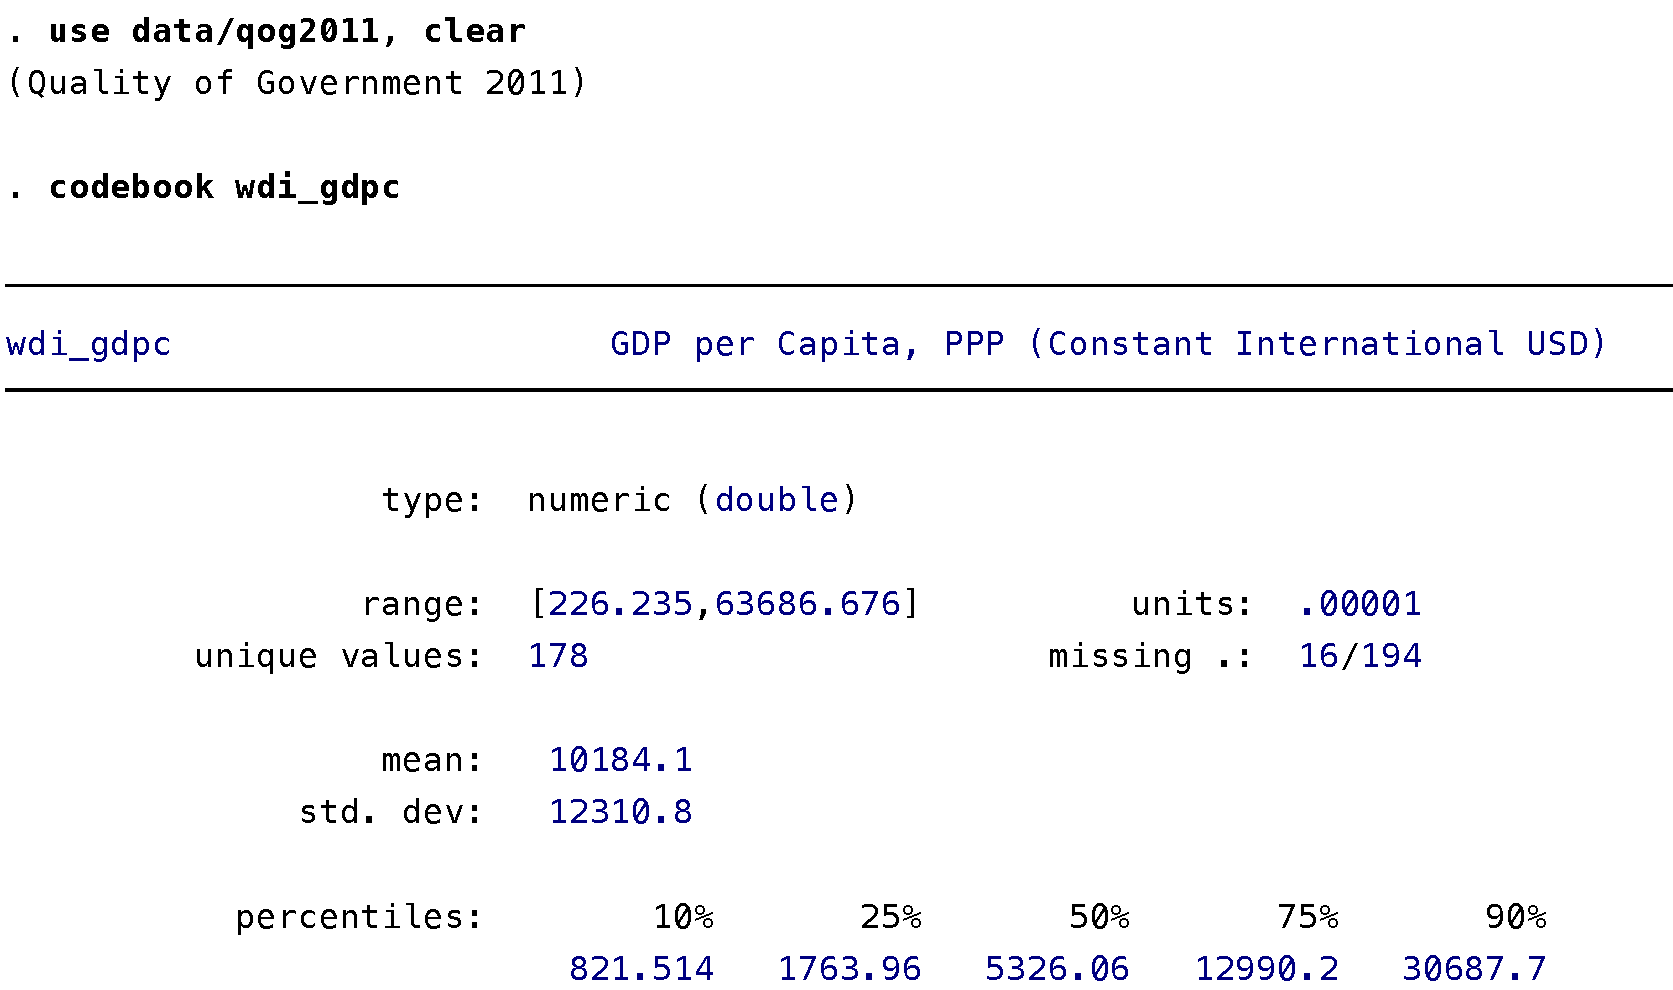
\includegraphics{qog-codebook-gdpc}\\[1em]
	
	We can now use the \cmd[su]{summarize} command to get the average height (measured in inches) and weight (measured in pounds) of U.S. residents over the past decade or so:
	
	\begin{docspec}
		use data/nhis9711, clear\\
		su weight height
	\end{docspec}
		
	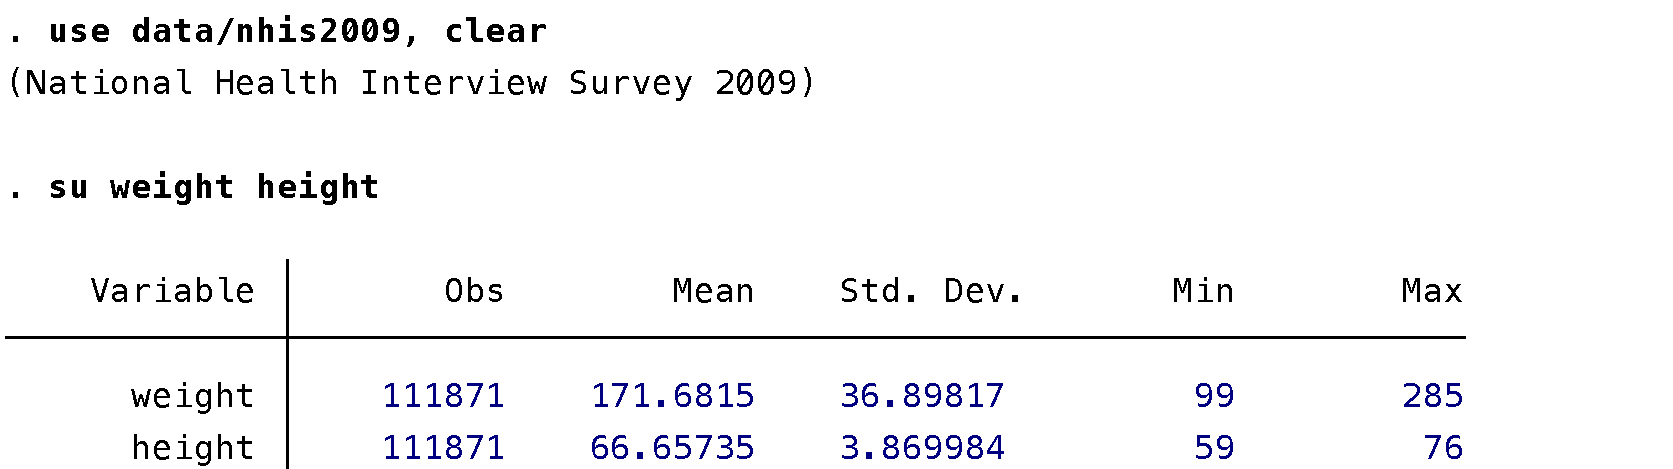
\includegraphics{nhis-su-height-weight}\\[1em]
	
	Using that combination of variables, we can generate the Body Mass Index of the sample population from its inch/pound equation. We then label the variable with an informative label and finally summarize the new variable with the \cmd[su]{summarize} command:\\[1em]
	
	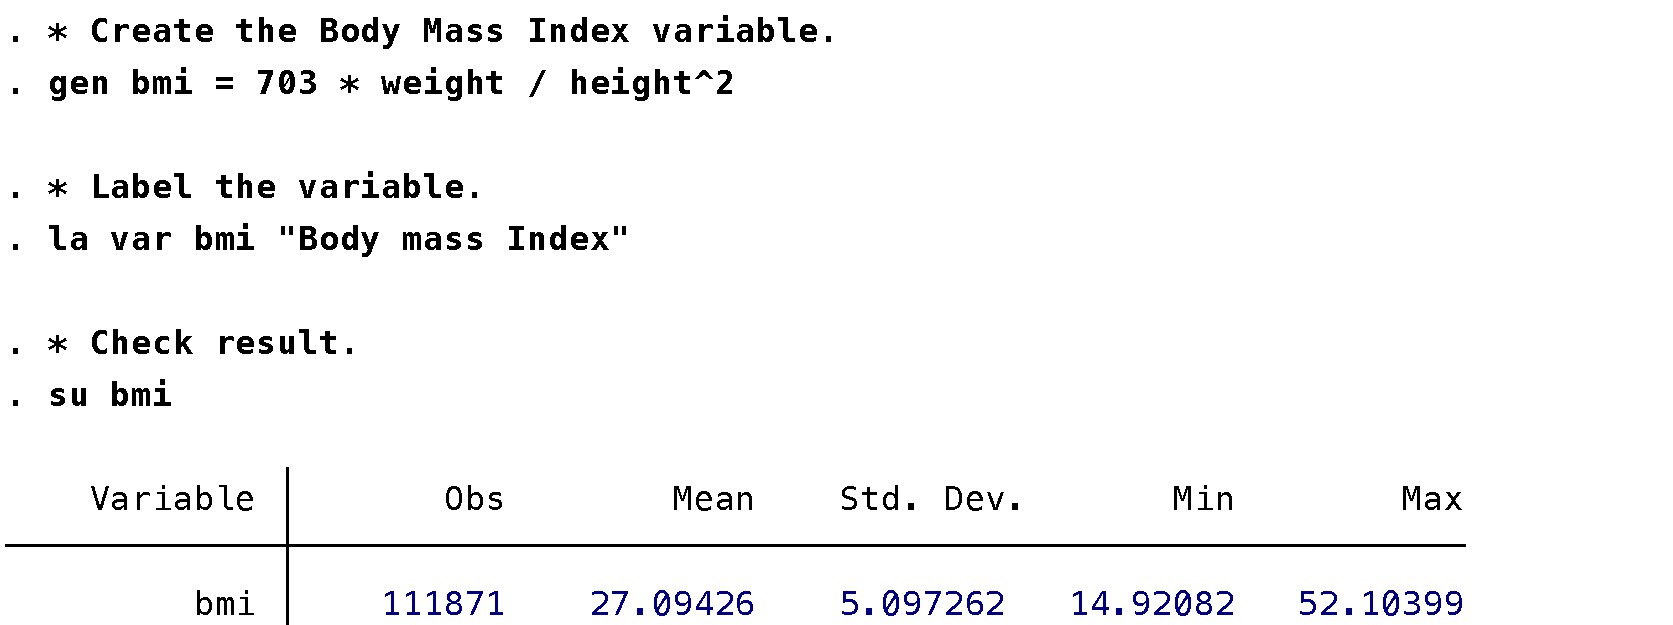
\includegraphics{nhis-gen-su-bmi}\\[1em]
	
	Using the \cmd[gen]{generate} and \cmd[su]{summarize} commands is probably the simplest routine to create and summarize a continuous variable. There are cases, however, where other commands are better tools for recoding a variable to a new one.
	
	\index{Variables!Categorical variables}%
	\item[Categorical variables] are artifical numeric codes for discrete entities that can be either ordered, like a 4-point scale of agreement to a question that goes from 1 `Strongly agree' to 4 `Strongly disagree', or unordered, like ethnicity, religious denomination, race or any other nominal marker for which there is no true ordering. These variables do not have meaningful averages but usually come with \emph{text labels} to describe each category: 1 will code for `Married', 2 for `Single', 3 for `Widowed', etc.

	A categorical variable might correspond to a continuous variable at lesser dimensionality: age groups, for example, are a recode of age measured in years into a handful of ordered categories (15-24, 25-34, etc.), which allow to speak in aggregates like `the youth', `the workforce' or `seniors'. In such \emph{ordinal} variables, the \emph{cutoff points} are expected to follow some kind of numeric convention: age groups might be coded per decade, income might be coded by decile or by bands of thousands of constant dollars, and so on.

	The example below shows the output of the \cmd{fre} command for a categorical variable from the \ess dataset.\pkgfirst{fre} Household net income, which was originally measured in country-specific units, was aggregated to deciles for cross-country comparability:\\[1em]

	\begin{docspec}
		use data/ess2008, clear\\
		fre hinctnta
	\end{docspec}

	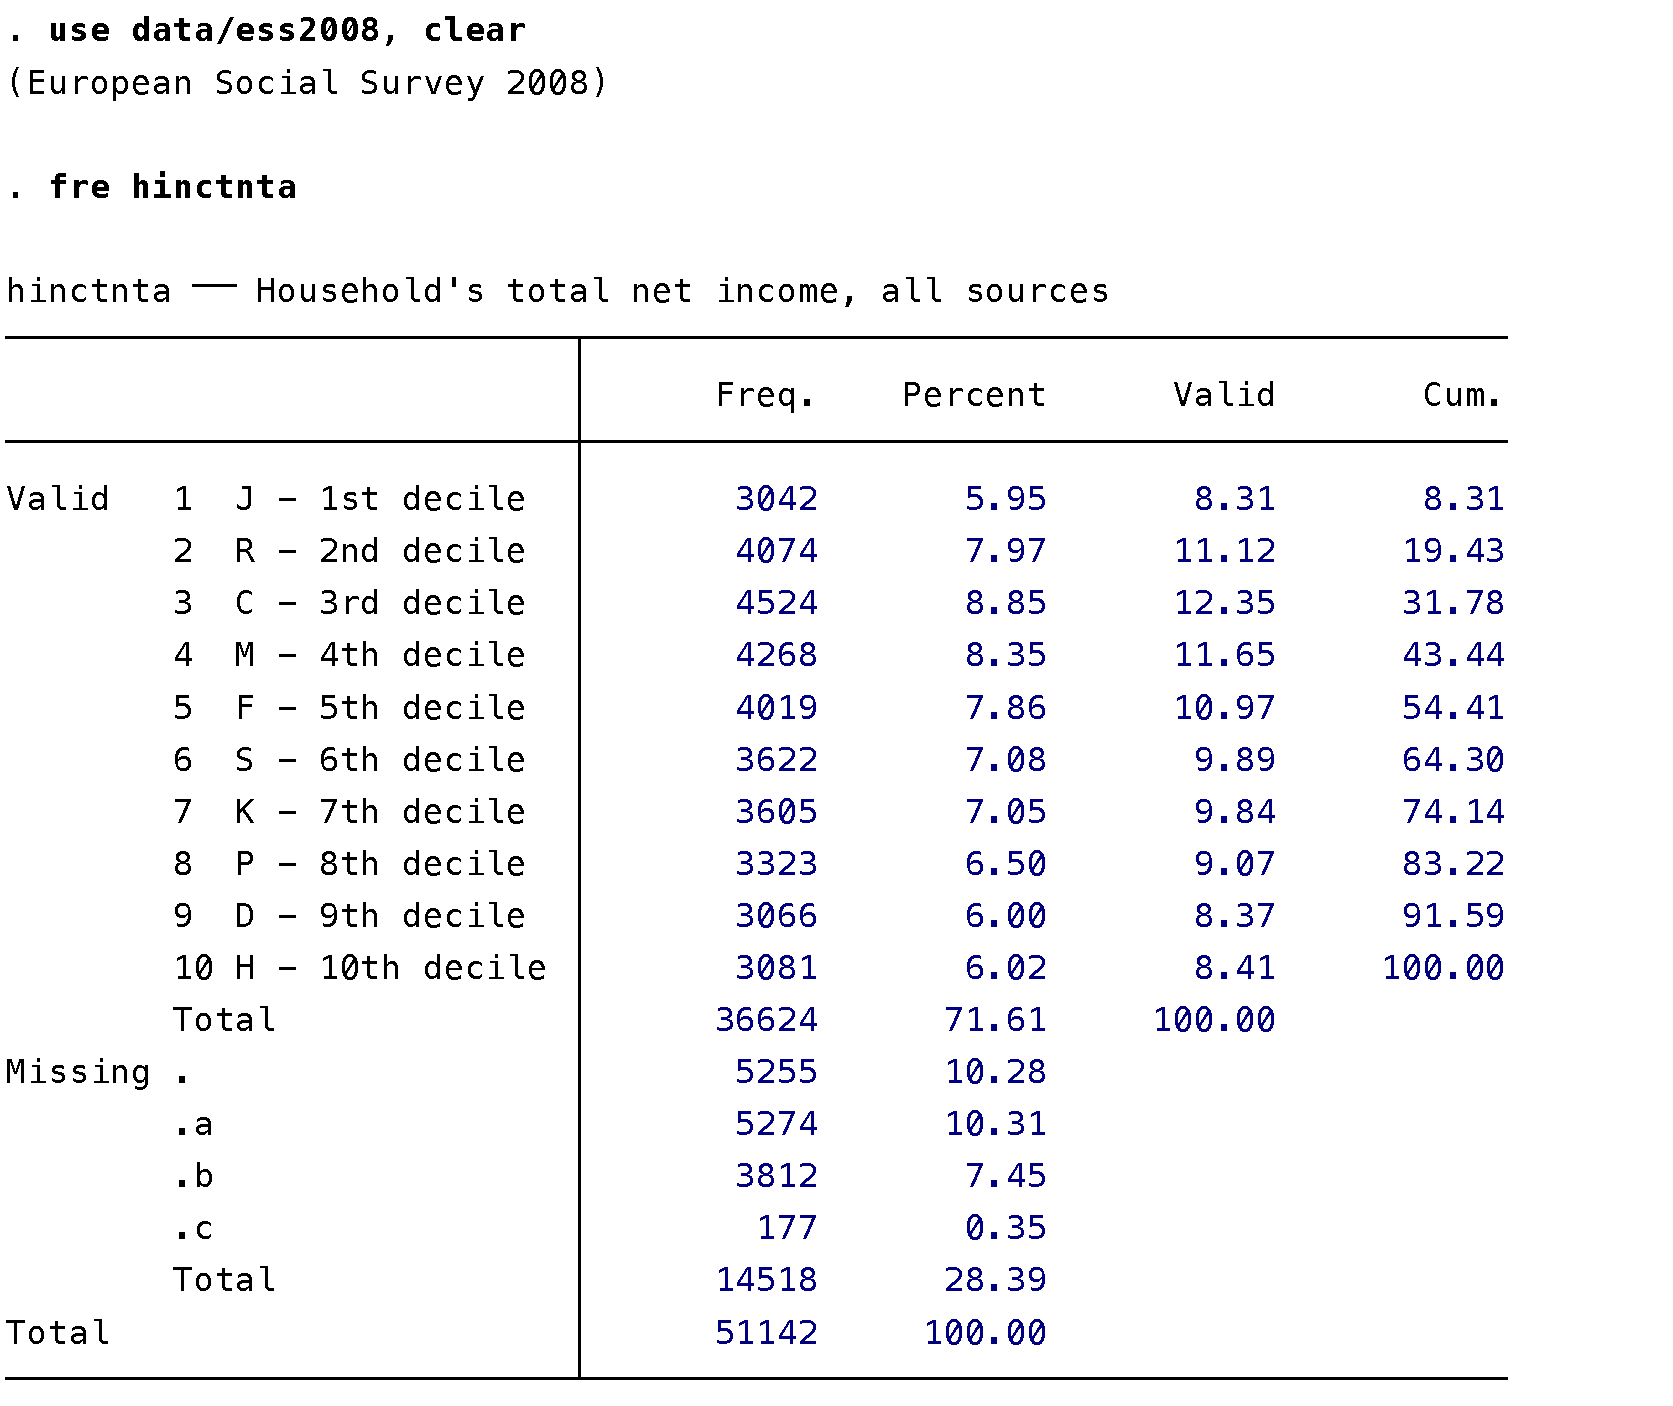
\includegraphics{ess-fre-hinctnta}\\[1em]
	
	Because the mean of a categorical variable does not reflect a true unit of measurement, it is not a useful descriptor: `the average age group is 4.5' is not a helpful statement. However, `the median age group' or `the modal age group' can be meaningful. This is because categorical variables can be described through \emph{relative frequencies}--generally \emph{percentages} (`40\% of political regimes are dictatorships') or \emph{fractions} (`half of the respondents are religious').

	In a categorical variable, the fraction of the sample taken by a category is its \emph{probability of occurrence}: if 45\% of the respondents are married, then the probability of being married among the respondents is $Pr(\mathrm{married}) = 0.45$. This is because categorical variables are best handled by thinking in terms of discrete probabilities: `percentages' are technically \emph{conditional probabilities}, and in a table, cell percentages are \emph{joint} probabilities and row or column percentages are \emph{marginal} probabilities.

	In the example below, \ess respondents were asked their feelings about their current household's income:\\[1em]
	
	\begin{docspec}
		use data/ess2008, clear\\
		fre hincfel
	\end{docspec}
	
	The largest group of respondents (the modal group), with 43\% of all responses, answered that they are `coping on present income'.\footnote{This group is also the group that contains the median respondent.} Since about 30\% of all respondents selected one of the last two response items, the probability for having difficulties living on current houseshold income is about $0.3$ among the (unweighted) sample of respondents:\\[1em]
	
	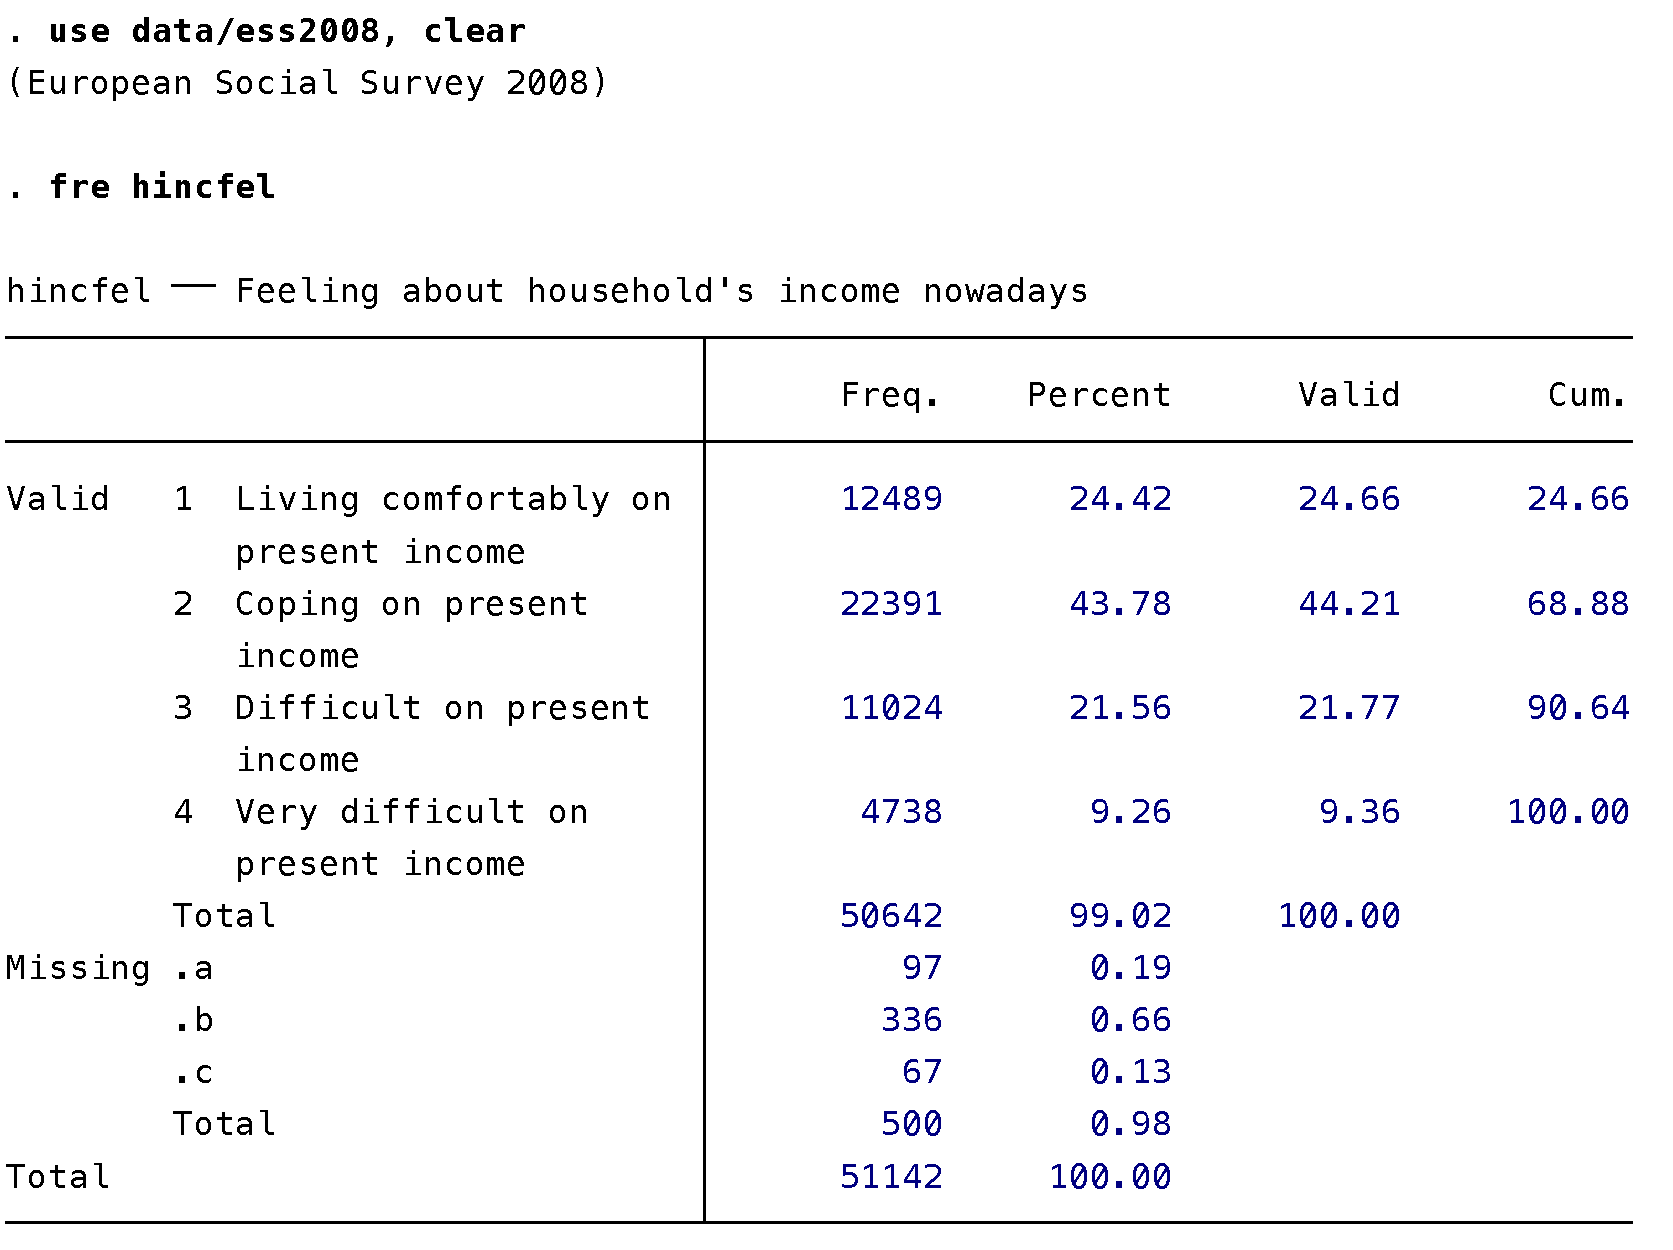
\includegraphics{ess-fre-hincfel}\\[1em]
		
	\index{Variables!Dummies (binary variables)}%
	\item[Dummies, or binary variables,] are categorical variables of the lowest possible dimensionality: they take only two values and therefore assert a logical statement: YES/NO, TRUE/FALSE, 0/1, male/female, married/single, democratic/dictatorial, etc. A convention is to name dummies after their true statement: a gender dummy called \texttt{female} codes 0 for `male' and 1 for `female'.
	
	The mean of a dummy is the fraction of the sample for which the logical statement is true. For example, if you code a dummy that holds 1 for `employed' and 0 for `unemployed' and the mean of that dummy, called \texttt{unemployed} so that its name denotes the true statement, is 0.18, then 18\% of the respondents have been reported or self-reported as unemployed (and the probability of being unemployed among the respondents is $Pr(\mathrm{unemployed}) = 0.18$. Dummies are particularly handy because of these `logical immediacy' characteristics.
	
	Here is an example of a \QOG dummy variable that codes for democratic status:\\[1em]
	
	\begin{docspec}
		use data/qog2011, clear\\
		fre chga\_demo
	\end{docspec}
	
	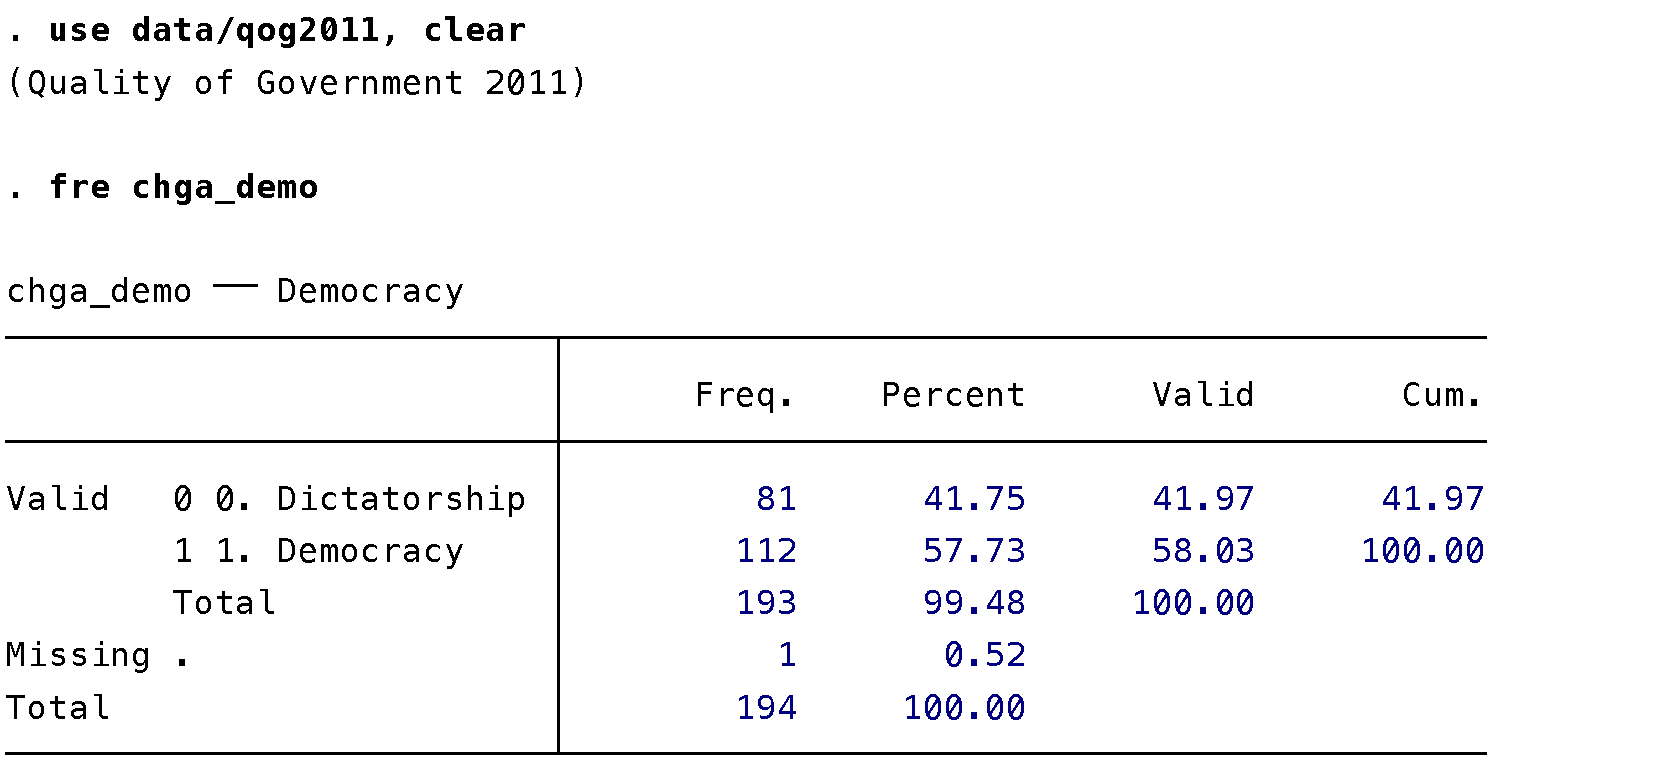
\includegraphics{qog-fre-chga_demo}\\[1em]
	
	In the example above, the variable could simply be renamed \texttt{democratic} and make immediate sense to the reader. It however often happens that dummies will be encoded as two `bland' items instead of having a logical sense, as in this \gss example:
	
	\begin{docspec}
		use data/gss2010, clear\\
		fre sex
	\end{docspec}
	
	It would be a good idea, in this case, to generate a meaningful dummy out of the existing one, using a logical statement to define the dummy, and excluding missing values from the process:%
		\label{female-dummy}
	
	\begin{docspec}
		* Create a female dummy.\\
		gen female:female = (sex == 2) if !mi(sex)\\[1em]
		
		* Label the values of the dummy.\\
		la def female 0 "Male" 1 "Female", replace\\[1em]
		
		* Check result.\\
		fre female
	\end{docspec}

	This example, which also appears in a Stata handbook by \cite{LongFreese:2001a}\footcite{FeinsteinThomas:2002d}, anticipates what we learn to do in the next sections with conditional statements, missing values and value labels. It takes the value 0 for males and 1 for females for nonmissing values of the \texttt{sex} variable, and then defines each value of the dummy through the \texttt{female} value label that has been assigned to the \texttt{female} dummy by the previous \cmd{gen}{generate} command:\\[1em]
	
	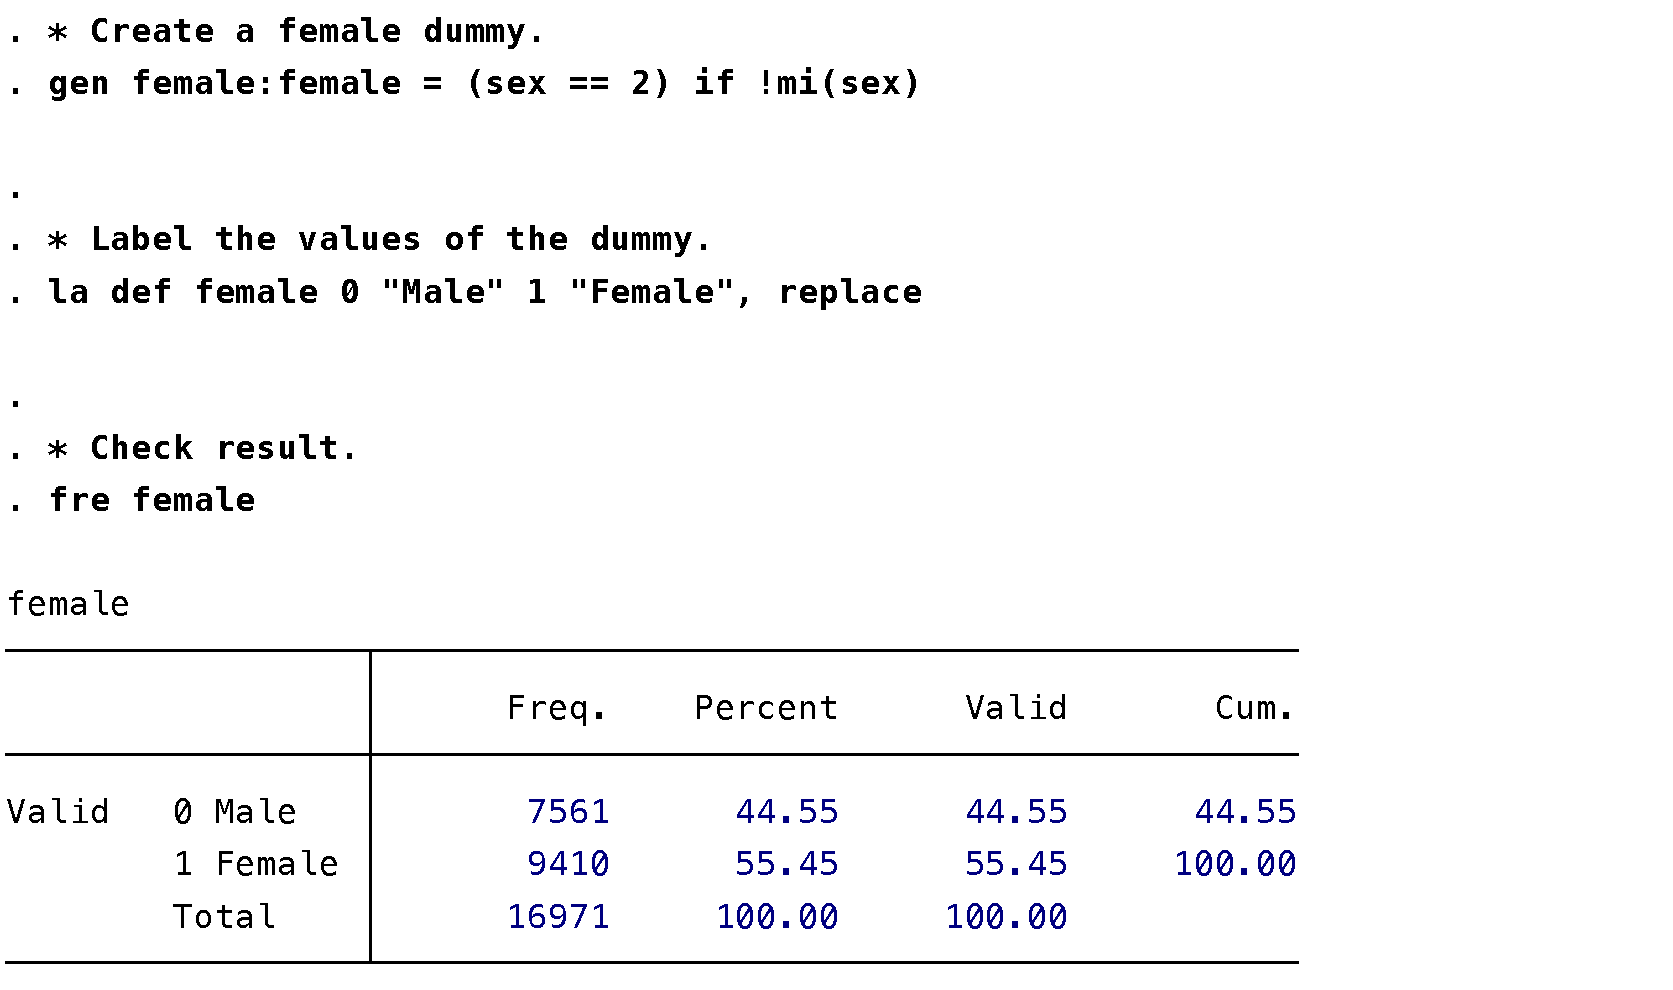
\includegraphics{gss-female-dummy}
	
	The percentages of a dummy are intuitively connected to its mean. If males are coded 0 and females 1, then the mean of the \texttt{female} variable is simply the ratio of females in the sample. The \cmd[su]{summarize} command provides the quickest way to compute this mean:
	
	\begin{docspec}
		* The mean of the dummy is the percentage of females.\\
		su female
	\end{docspec}

	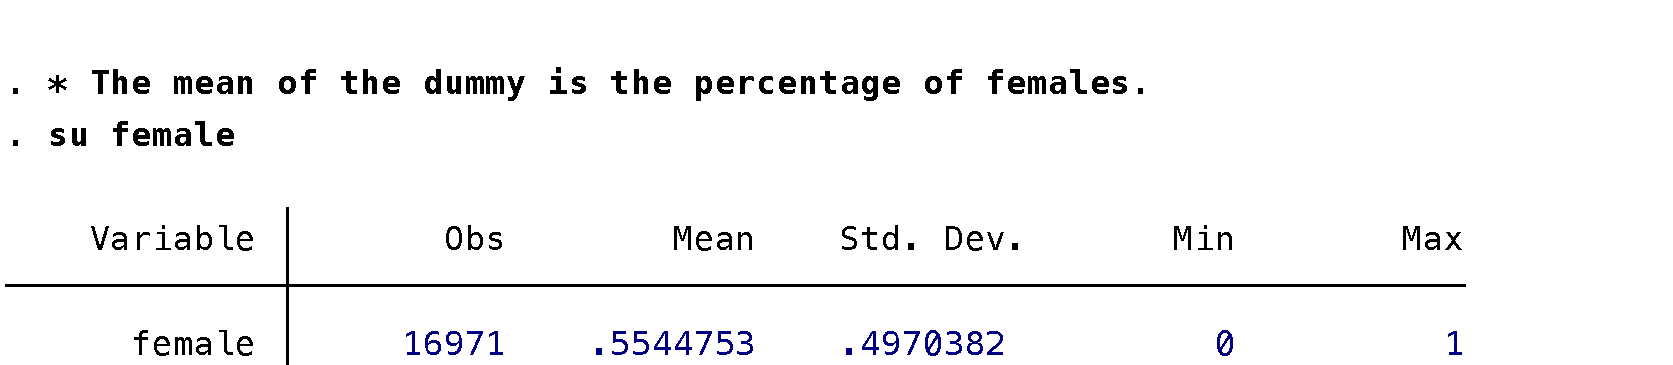
\includegraphics{gss-female-mean}
	
	The unweighted years of \GSS data used in the course have a slight excess representation of females, which is not unusual in survey data. This could be corrected, as most of our estimates could be, by using survey weights and a more complex survey design, set with the \cmd{svyset} command. The crude estimate, however, is generally enough for our purposes.\\[1em]

\end{description}

\newthought{Schematically}, continuous variables have mostly quantitative properties (meaningful units, infinite values, …), and categorical variables have mostly qualitative properties (their numbers code substantive groups or categories), whereas dummies have mostly logical properties.

You want to remember that terminology to understand what kind of distribution and summary statistics are appropriate to describe each type of variable, and then later how to plug each type of variable into a statistical test or model.

Accept some flexibility in classification: `continuous' and `categorical' denote abstract properties. Any physical variable is only imperfectly continuous from a mathematical perspective, and many ordinal variables with a large number of categories can be treated as continuous in practice.

Before you even start worrying about recoding continuous to categorical variables, let's cover missing values, as they work (almost) identically for all variables.

%
%
% 1.2 ==========================================================================
%
\subsection{Missing values}
\label{sec:missing-values}

\newthought{Missing values} are a consequence of survey nonresponse, coding errors and insufficient data. They might be coded with acronyms like `DK' (``don't know'') or `NA' (``no answer'' or ``not applicable''), or with numeric codes like -1 or 99. Observations that have missing values cannot be considered for the kind of analysis that we will later run, and we will eventually have to subset the data to exclude them from the sample.

\newthought{Stata requires missing values to be encoded} as dots ("\texttt{.}") that can be followed by a letter, as in "\texttt{.a}", "\texttt{.b}", ..., "\texttt{.z}". Any other value coding for missing values in the data has to be correctly recoded to `dot' encoding before the data is to be used in Stata, or summary statistics (among other things) will be wrongly reported. We show three different ways to recode missing values below.

\begin{description}
	\item[Selectively cloning a variable]%
	%
	A simple case of a missing value recode is when a variable needs to get trimmed from badly encoded missing values. Below is an example from the \NHIS dataset, where the last value for marital statuts is actually a missing value:

	\begin{docspec}
		use data/nhis9711, clear\\
		fre marstat
	\end{docspec}

	The issue is easy to diagnose with the \cmd{fre} command. It takes two built-in commands, \cmd[tab]{tabulate} and \cmd[la li]{label list}, to get the same output, so \cmd{fre} is always worth using to look at variable encoding:\\[1em]

	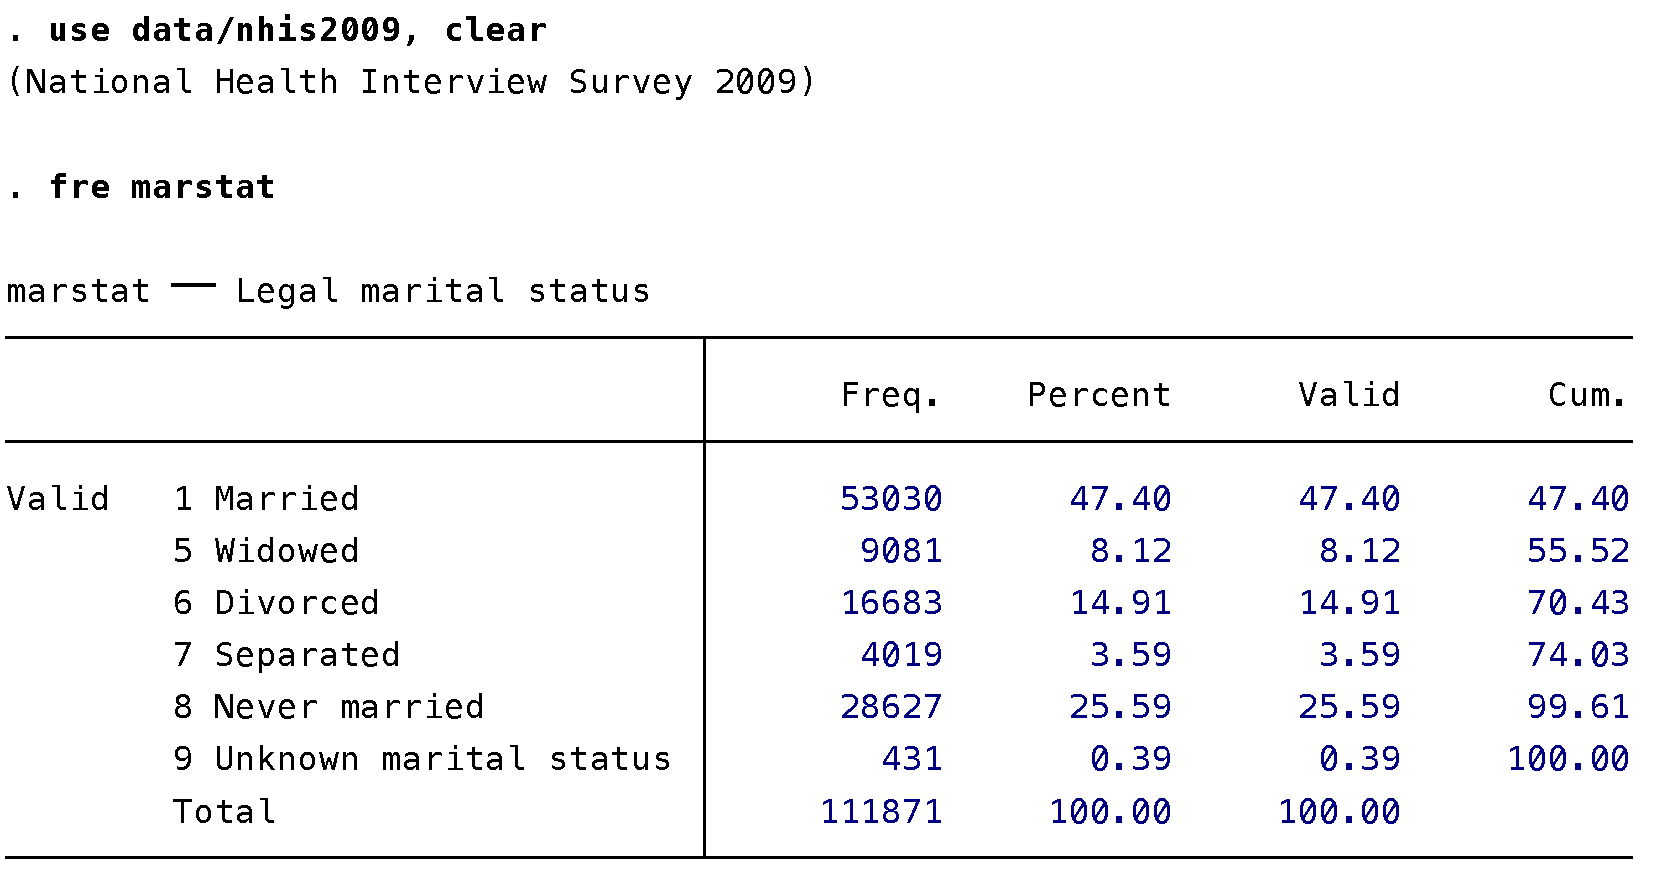
\includegraphics{nhis-fre-marstat}\\[1em]

	When the variable has labels that you want to preserve, the \cmd{clonevar} command lets you exclude the missing values and copy exactly everything else from the old variable to a new one, as shown below where we create the \texttt{marital} variable:

	\begin{docspec}
		clonevar marital = marstat if marstat < 9\\
		fre marital
	\end{docspec}

	All values and value labels (`Married', `Widowed', etc.) have been preserved in the new variable, at the exception of the 431 respondents of unknown marital status, who are now identified as missing by Stata:\\[1em]

	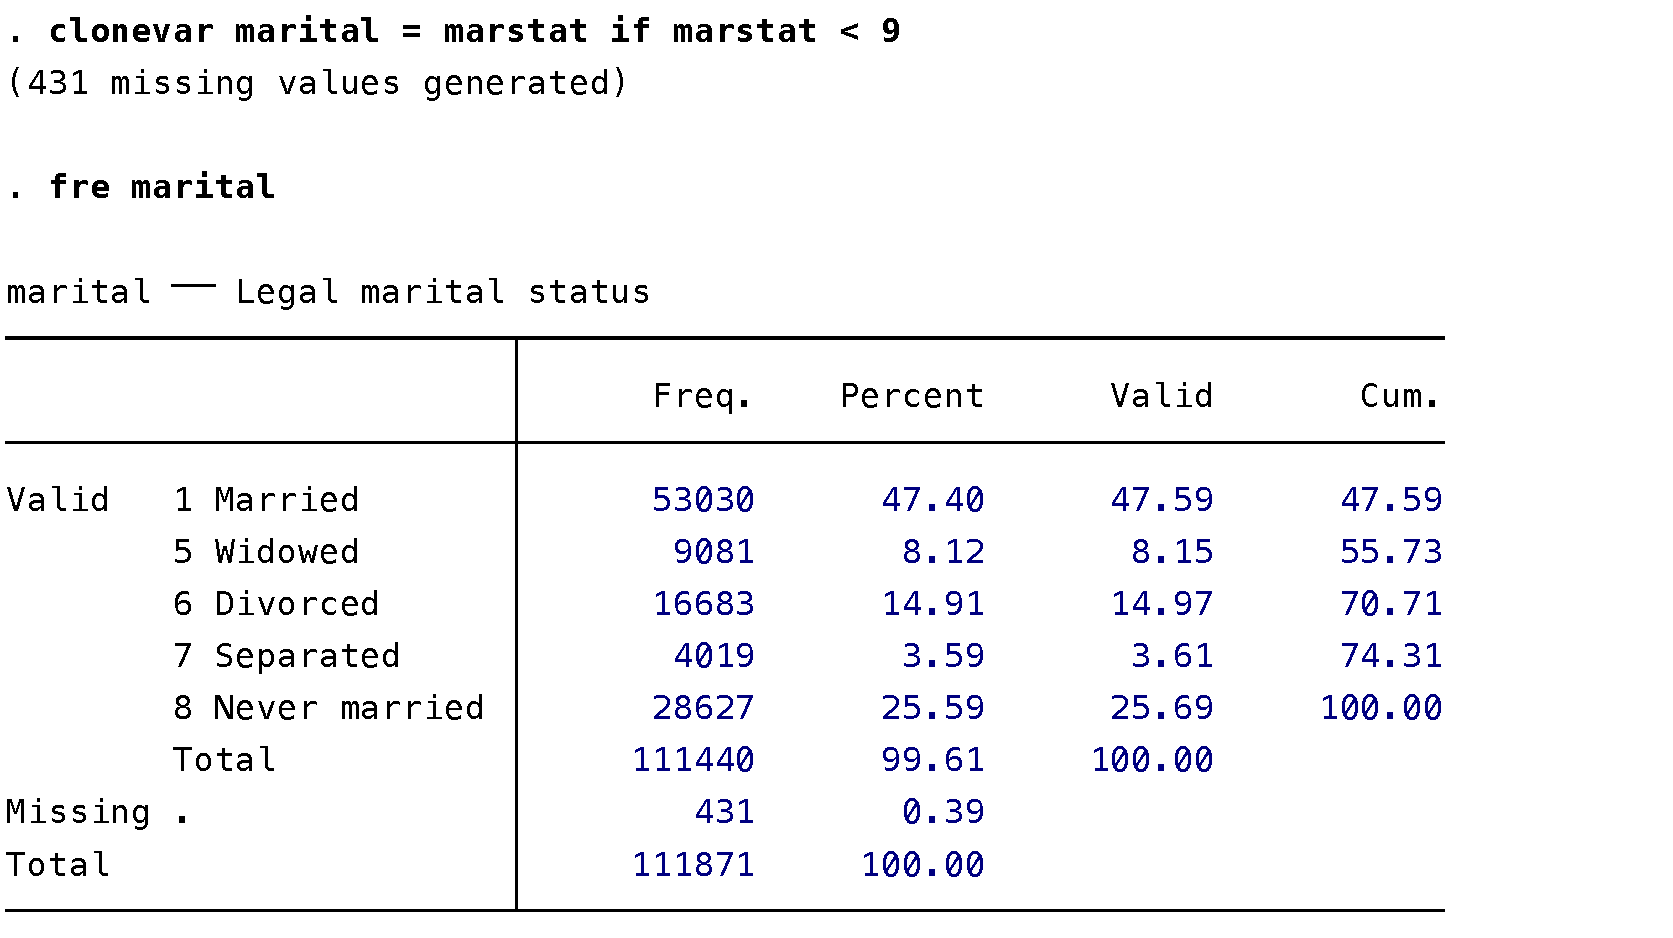
\includegraphics{nhis-clonevar-marital}\\[1em]

	\item[Selectively duplicating values]%
	%
	When the variable does not have labels, you can be most straightforward and use the \cmd[gen]{generate} command to recode specific values to missing. Our example for such an operation shows the coding of the age variable in the \wvs:

	\begin{docspec}
		use data/ess0810, clear\\
		fre edulvla, nomissing nowrap
	\end{docspec}
	
	We use the \cmd{fre} command to diagnose the issue, passing the \coab{r}{rows}{fre} option in order to show only a few values instead of the full range from 15 to 99. Strangely enough, values 98 and 99 indicate missing data here:\\[1em]

		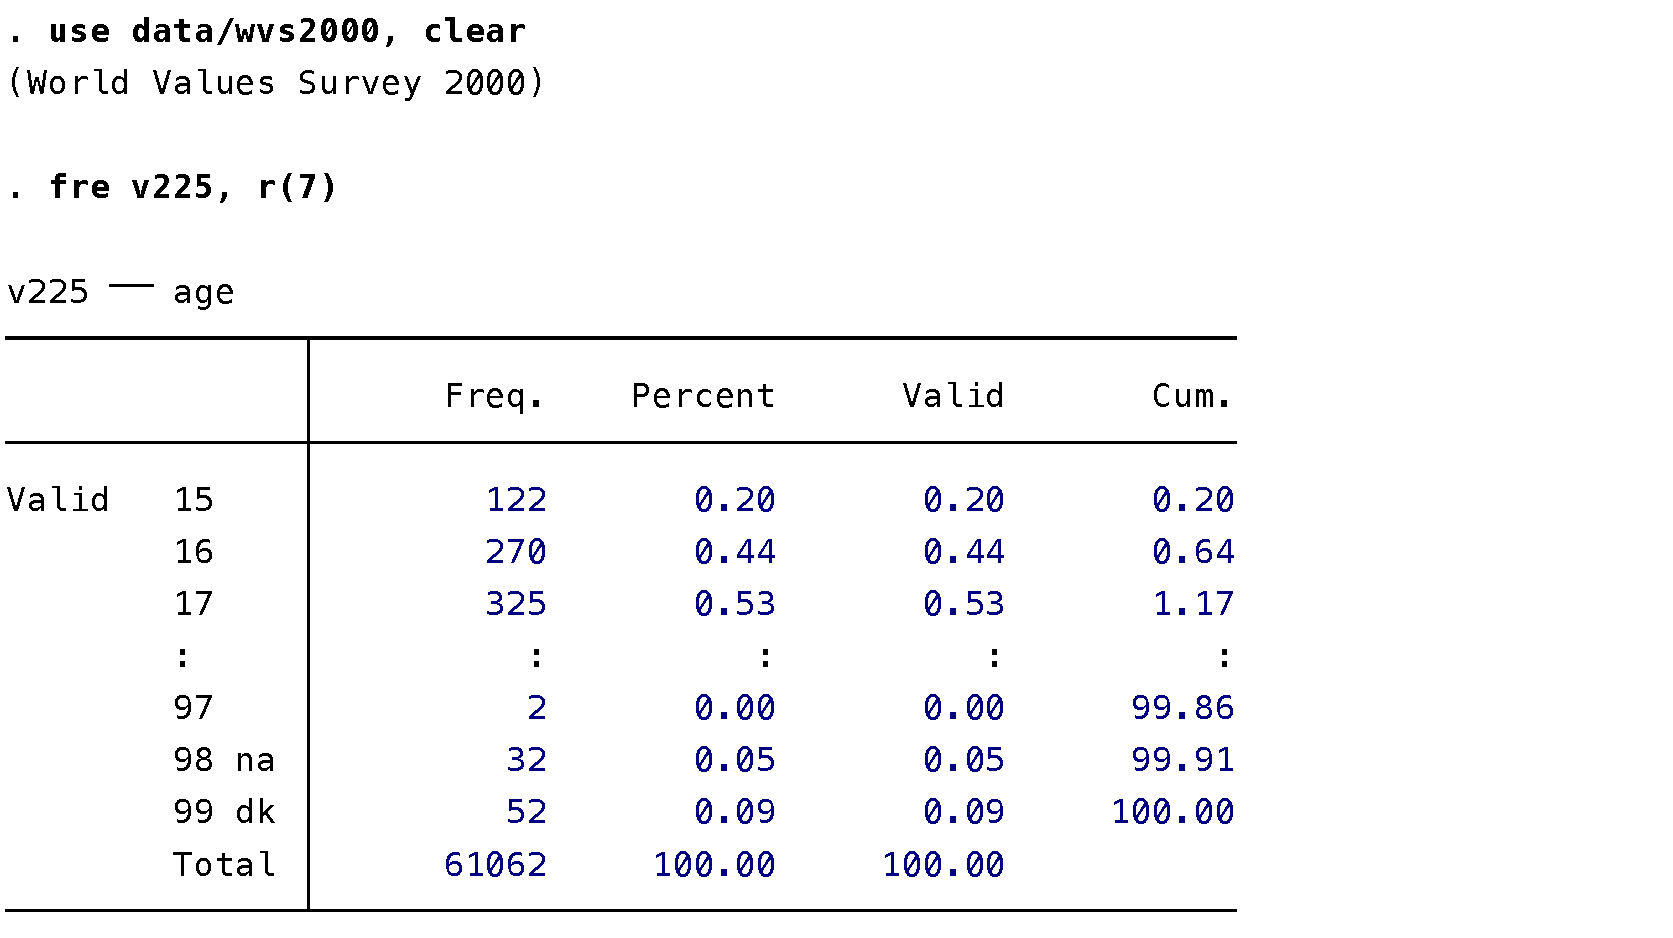
\includegraphics{wvs-fre-age}\\[1em]
	
	This error can be fixed simply by recomputing an age variable that excludes the upper categories with the \cmd[gen]{generate} command, which duplicates the nonmissing values and allows to pick up a better name for the variable all at once:

	\begin{docspec}
		gen edu = edulvla if edulvla < 55\\
		fre edu, nomissing nowrap
	\end{docspec}

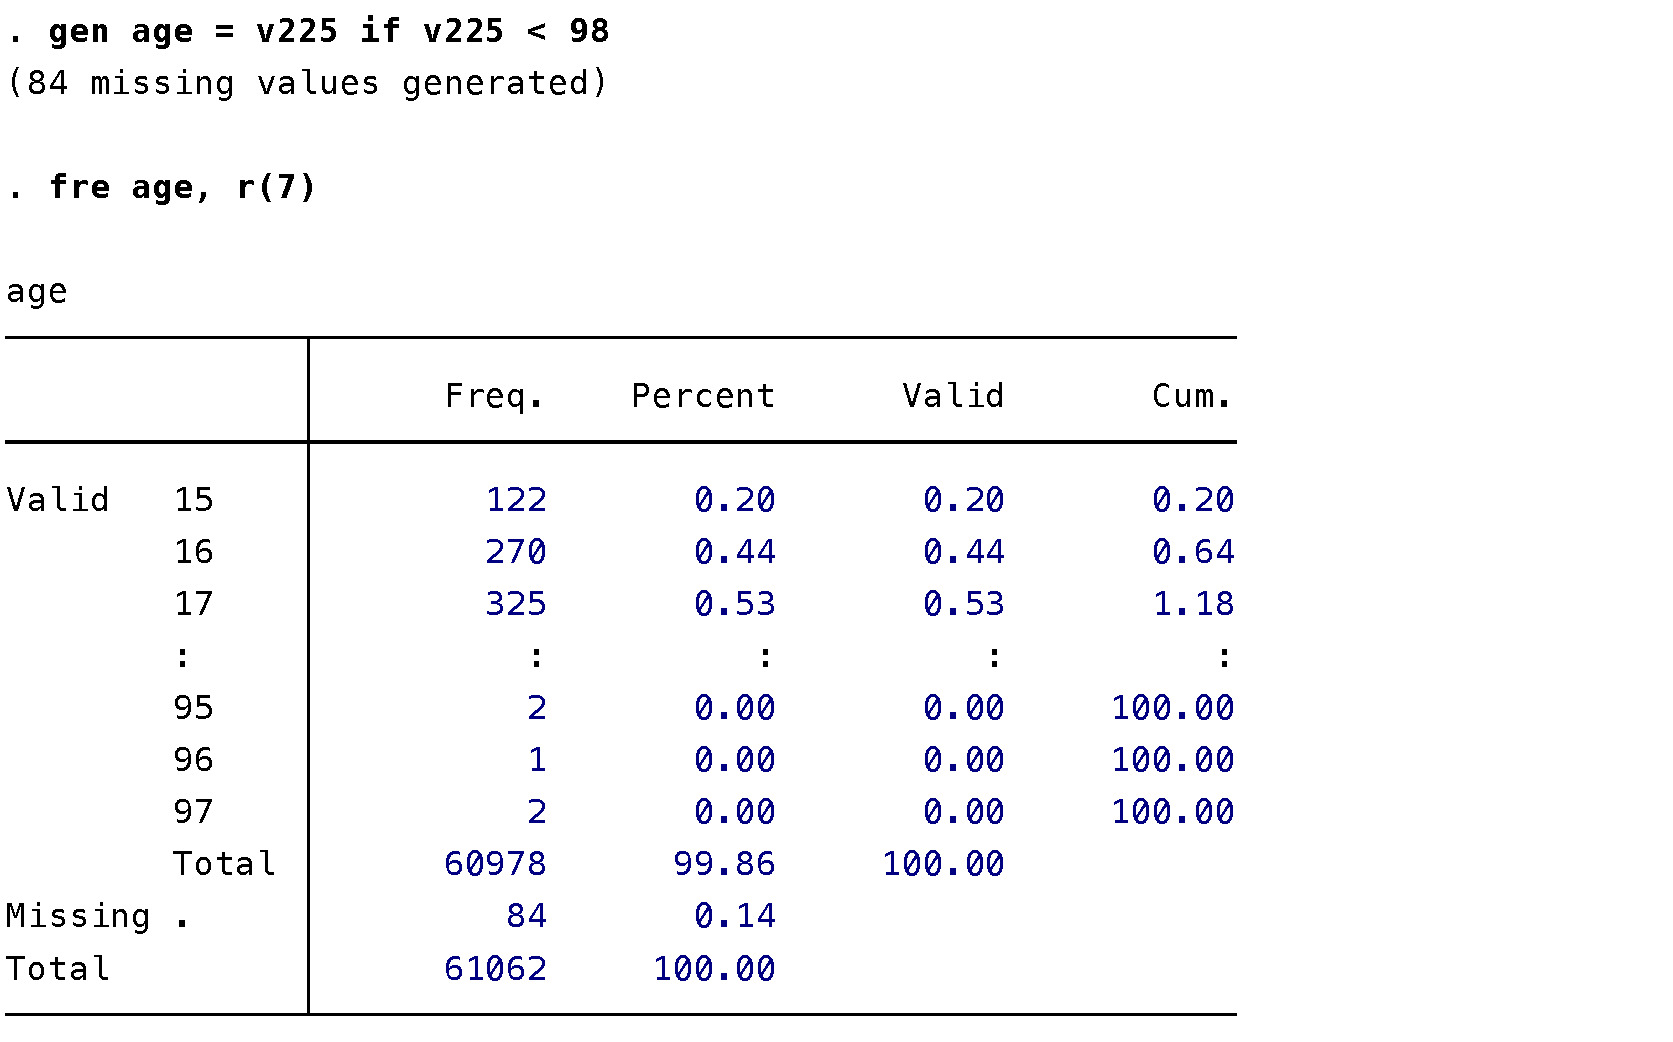
\includegraphics{wvs-gen-age}\\[1em]

	\item[Batch encoding of missing values]%
	%
	The \cmd{clonevar} and \cmd[gen]{generate} methods lose in efficiency if you are recoding missing values that follow the same coding scheme from one variable to another. The example below illustrates that situation with two \NHIS variables:\\[1em]

	\begin{docspec}
		use data/ess0810, clear\\
		fre edulvla eisced, nomissing nowrap
	\end{docspec}
	
	The\texttt{pooryn} and \texttt{uninsured} are both using \texttt{9} as a missing value.
	
	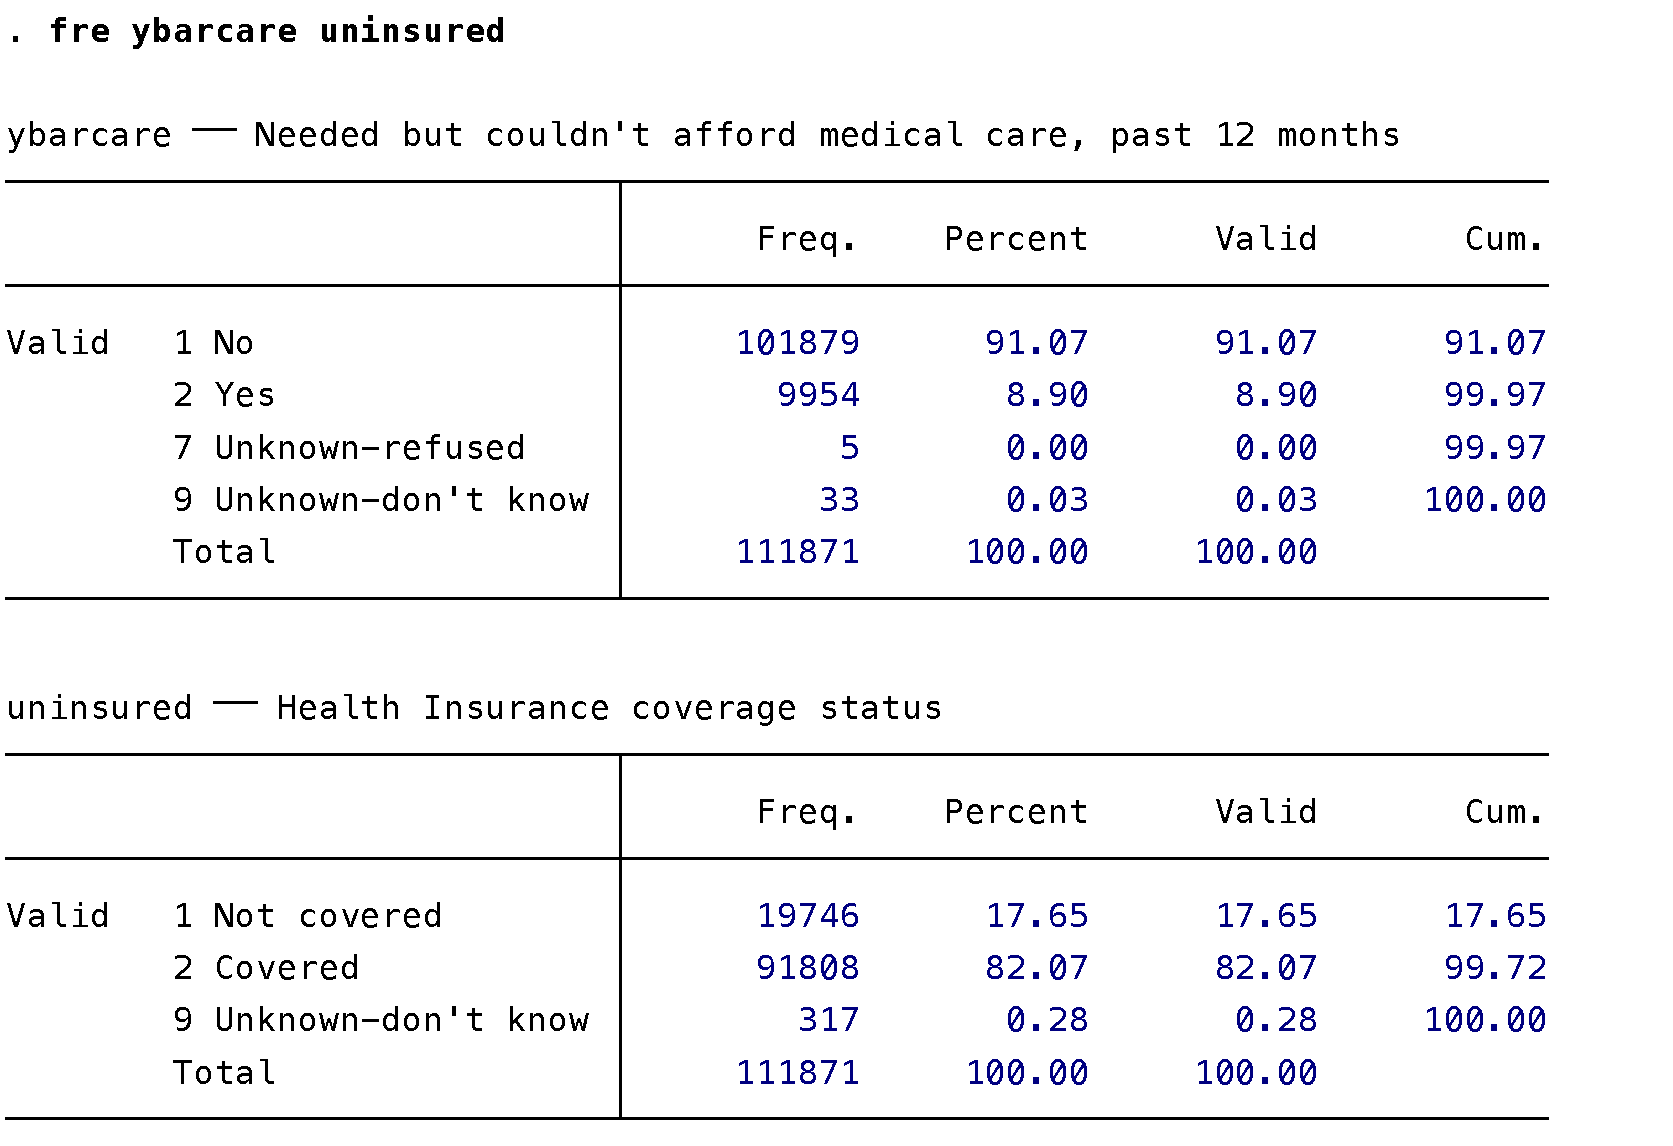
\includegraphics{nhis-fre-ybarcare-uninsured}\\[1em]

	In that case, the \cmd{mvdecode} command is quicker at coding these values to missing directly within the variables. The command works by specifying which variables are concerned, and what values should be recoded to missing:

	\begin{docspec}
		* Recode missing values of insurance and medical care.\\%
		mvdecode edulvla eisced, mv(55)\\[1em]%
		%
		* Check results.\\%
		fre edulvla eisced, nomissing nowrap\\%
	\end{docspec}
	
	Use this command with caution, as it makes it easy to recode erroneously, and systematically check your batch recodes:\\[1em]%

	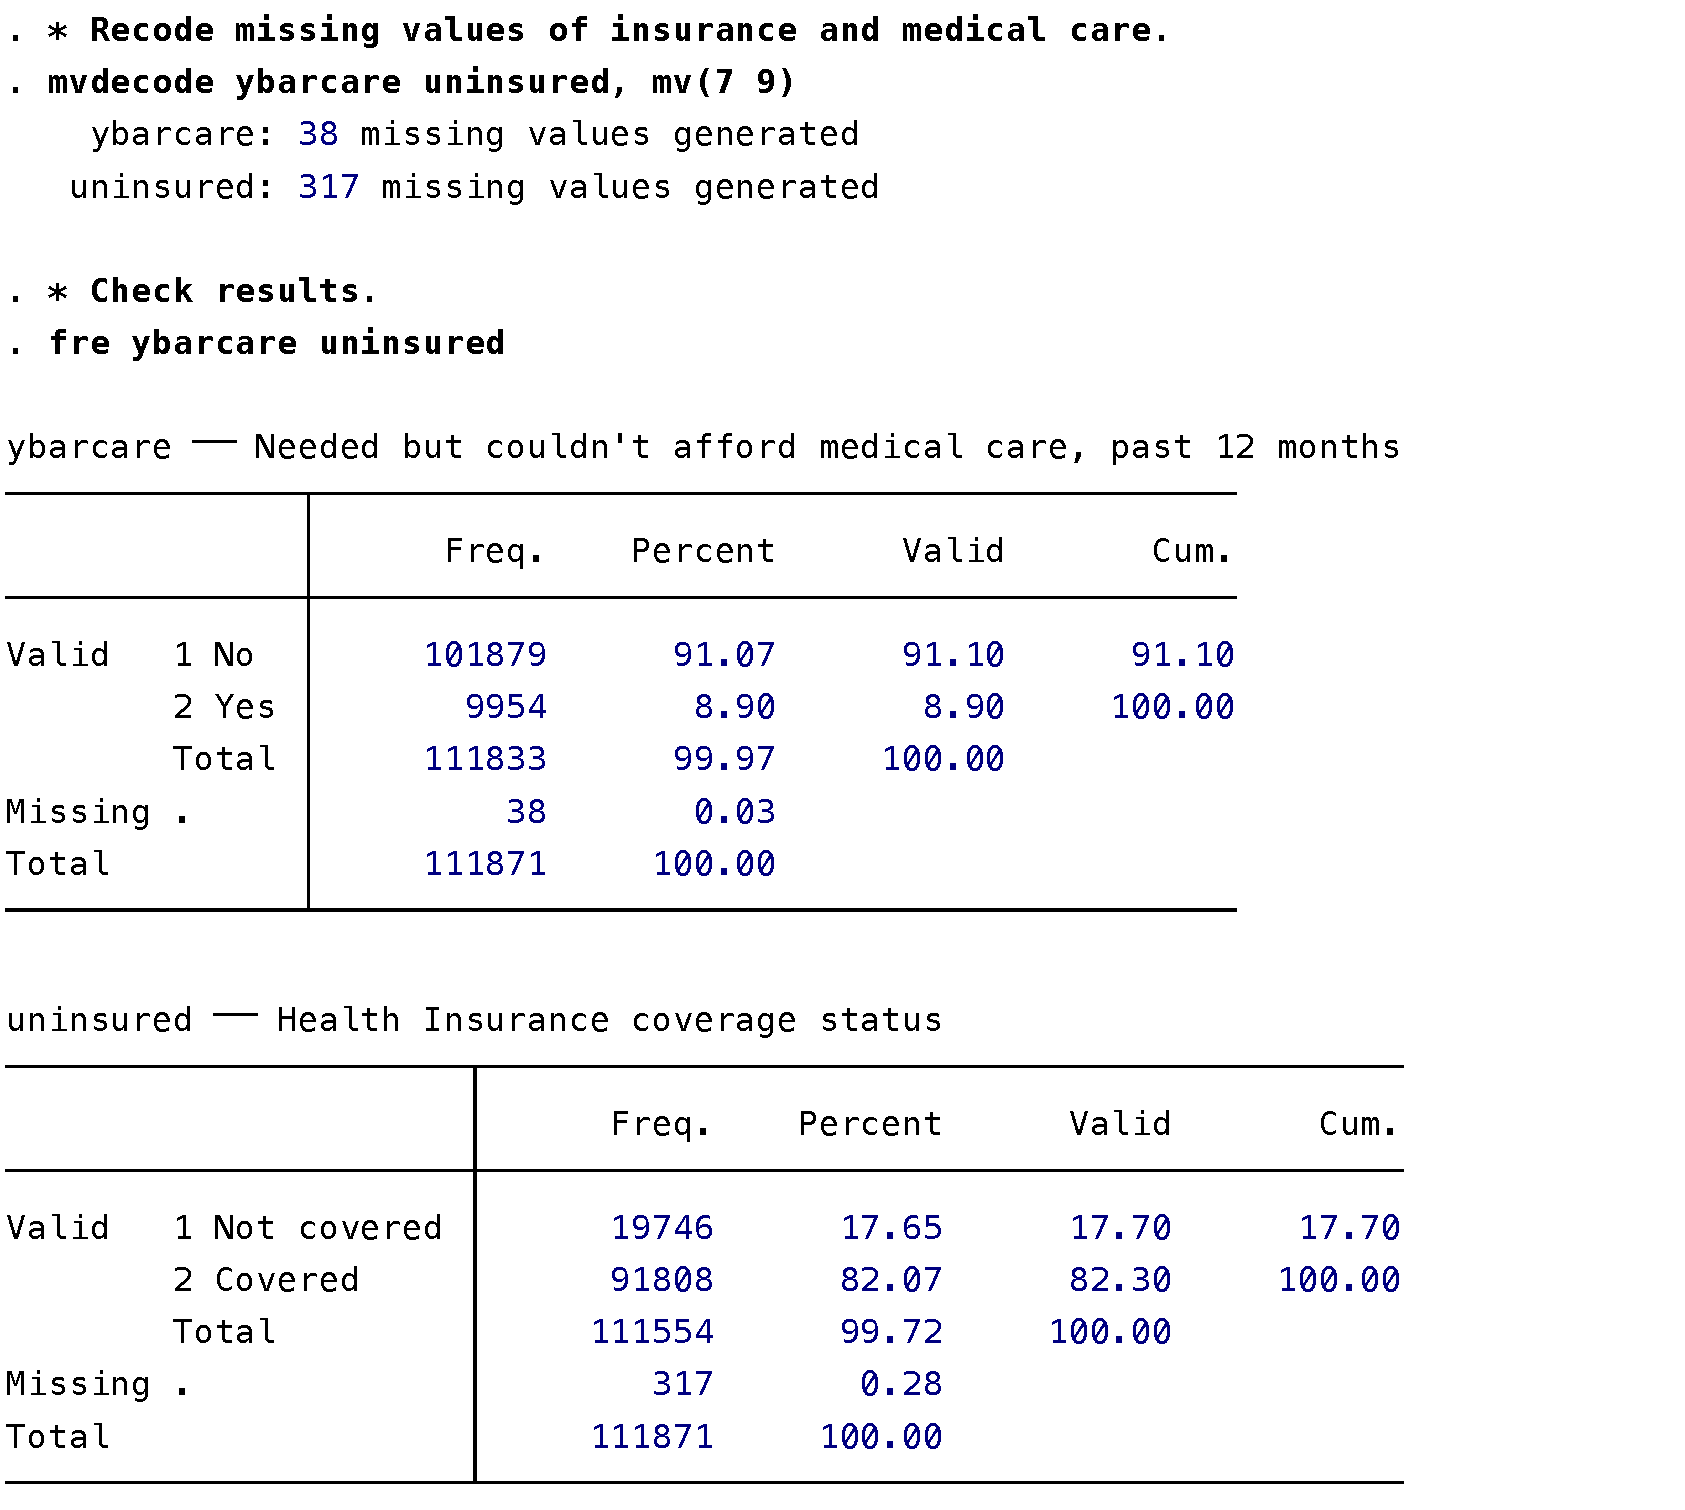
\includegraphics{nhis-recoded-ybarcare-uninsured}
\end{description}

\paragraph{Using logical operators} %
As previously with the female dummy recode from p.~\pageref{female-dummy} we have used a logical statement with the \cmd{if} command, to operate a command only for a selection of observations. The one above says: ``apply (the \texttt{clonevar} command) only to observations for which (marital status) is strictly inferior to 9''. A list of Stata logical statements is shown below:

\begin{table}
	\begin{center}
  	\footnotesize
  	\begin{tabular}{ll}
    	\toprule
    	Symbol & Meaning \\
    	\midrule
    	\quad \texttt{>} and\texttt{>=} & strictly superior / or equal to \\
    	\quad \texttt{<} and\texttt{<=} & strictly inferior / or equal to  \\
    	\quad \texttt{==} & equal to \\
    	\quad \texttt{!=} & \emph{not} equal to \\
    	\quad \texttt{mi(x, y, z)} & missing any of the variables\texttt{x, y, z}\\
    	\quad \texttt{!mi(x, y, z)} & \emph{not} missing any of the variables\texttt{x, y, z}\\
    	\quad \texttt{inlist(x, ...)} & values of variable \texttt{x} in the list \texttt{...}\\
    	\quad \texttt{if (...) \& (...)} & if (...) \emph{and} (...)\\
    	% \quad \texttt{if (...) | (...)}  & if (...) \emph{or} (...)
    	\bottomrule
  	\end{tabular}
	\end{center}
	\label{tbl:logical-symbols}%
		\index{Logical statements}\index{Selectors!Logical conditions: \cmd{if}}
\end{table}
	
\newthought{Once missing values are encoded}, you will have to subset your data, that is, to extract the set of observations for which no values are missing in the data. The \cmd{misstable pat} command provides a handy way to establish, as in the \ESS example below, the percentage of fuly measured observations:

	\begin{docspec}
		use data/ess0810, clear\\
		misstable pat agea gndr edulvla hinctnta
	\end{docspec}
	
	For the purpose of this example, the \cmd{misstable pat} command is shown immediately after data loading, but you should run it after recoding missing values to make sure that the subset works properly. The result is a table that provides the percentage of `full data' and indicates which variables have missing values:\\[1em]
	
	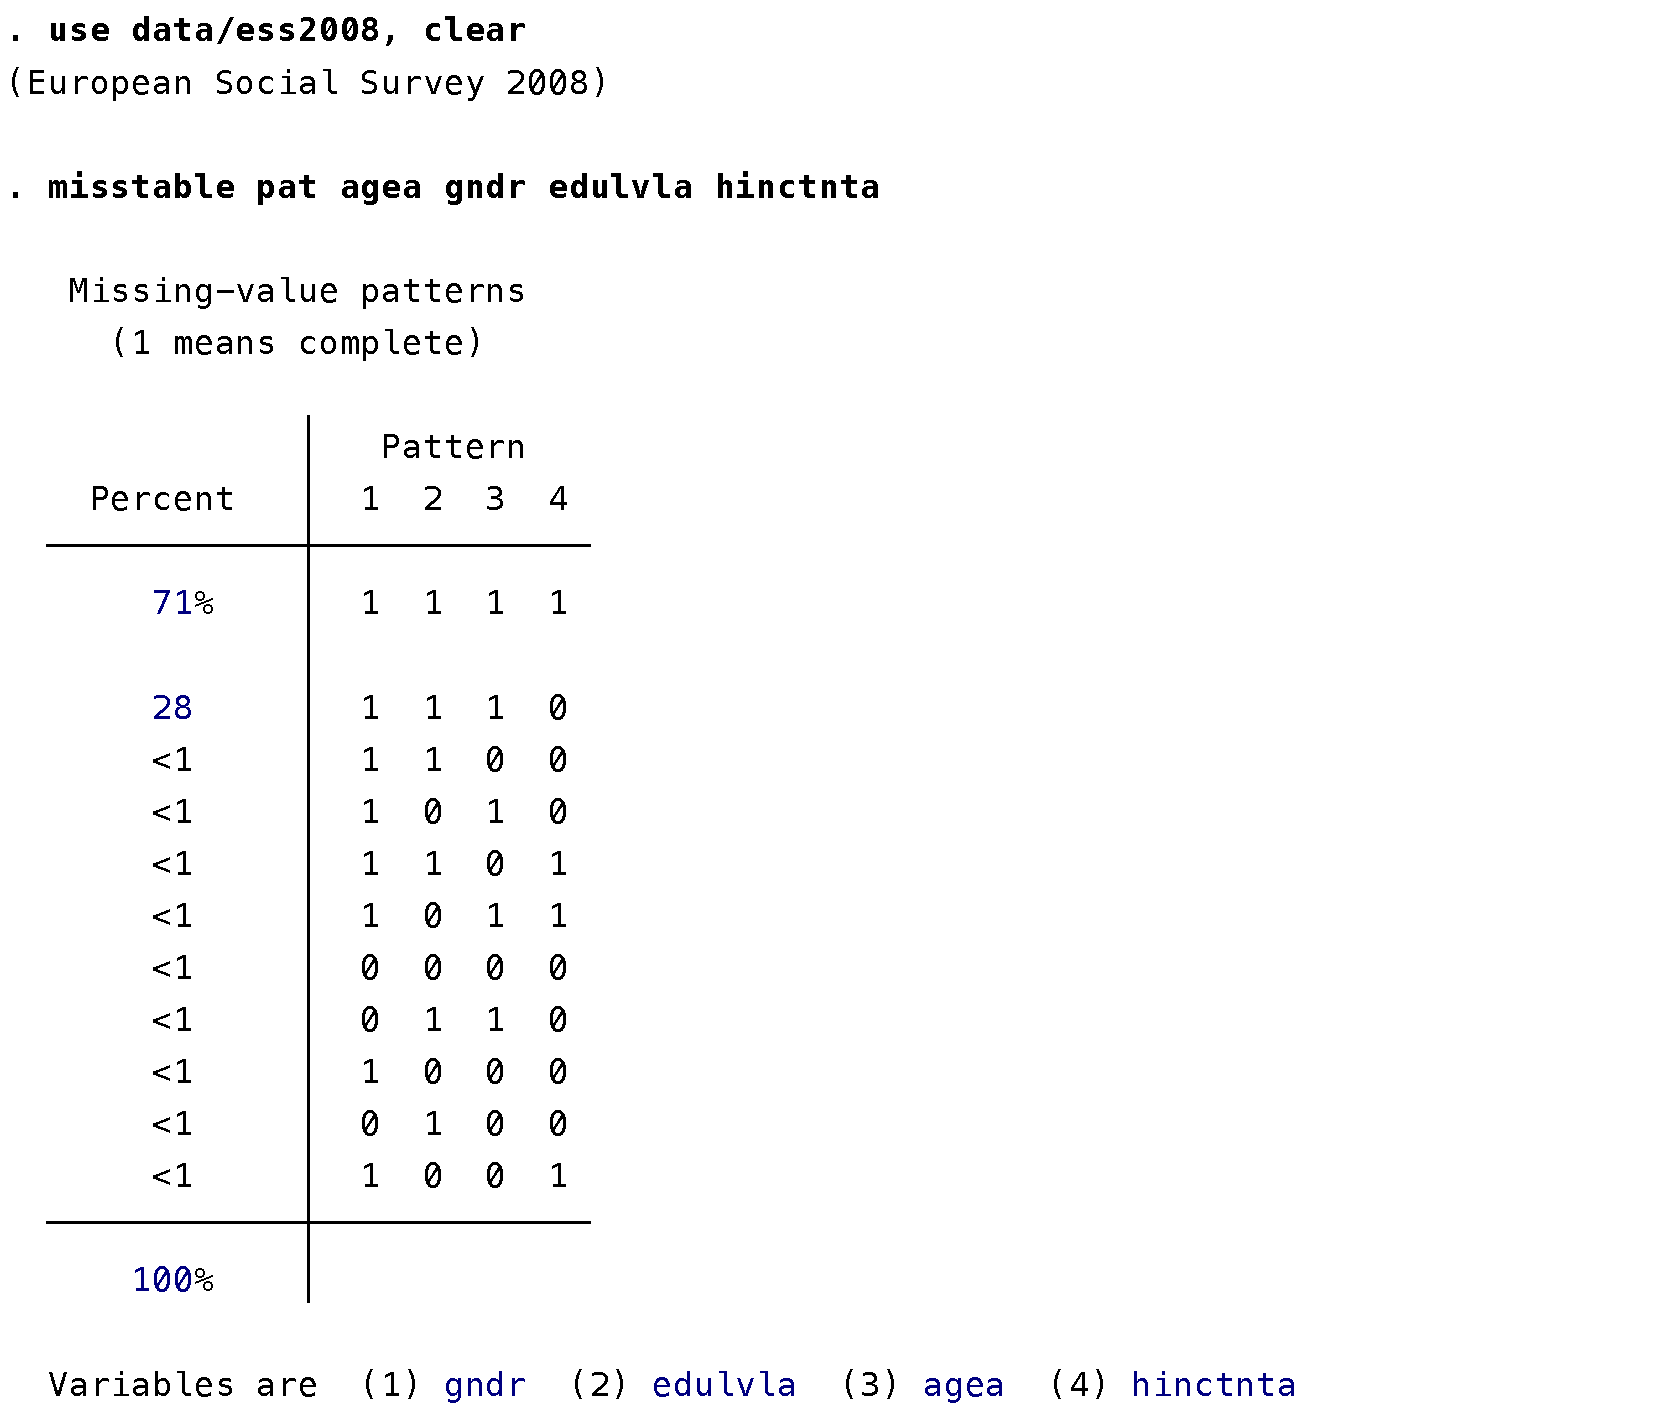
\includegraphics{ess-misstable-pat}\\[1em]

	The \cmd{misstable pat} command should be used at the right level of precision. For example, when working on comparative country case studies, you should specify each country separately to spot variations in missing values among the case studies:\\[1em]
	
	\begin{docspec}
		use data/ess0810, clear\\[1em]%
		%
		* Missing values for Germany.\\%
		misstable pat agea gndr edulvla hinctnta if cntry == "DE"\\[1em]%
		%
		* Missing values for Turkey.\\%
		misstable pat agea gndr edulvla hinctnta if cntry == "TR"
	\end{docspec}

	In this example, the country variable is not encoded but provided as text (string data) instead, which is why we can designate the countries directly by their acronyms between quotes:

	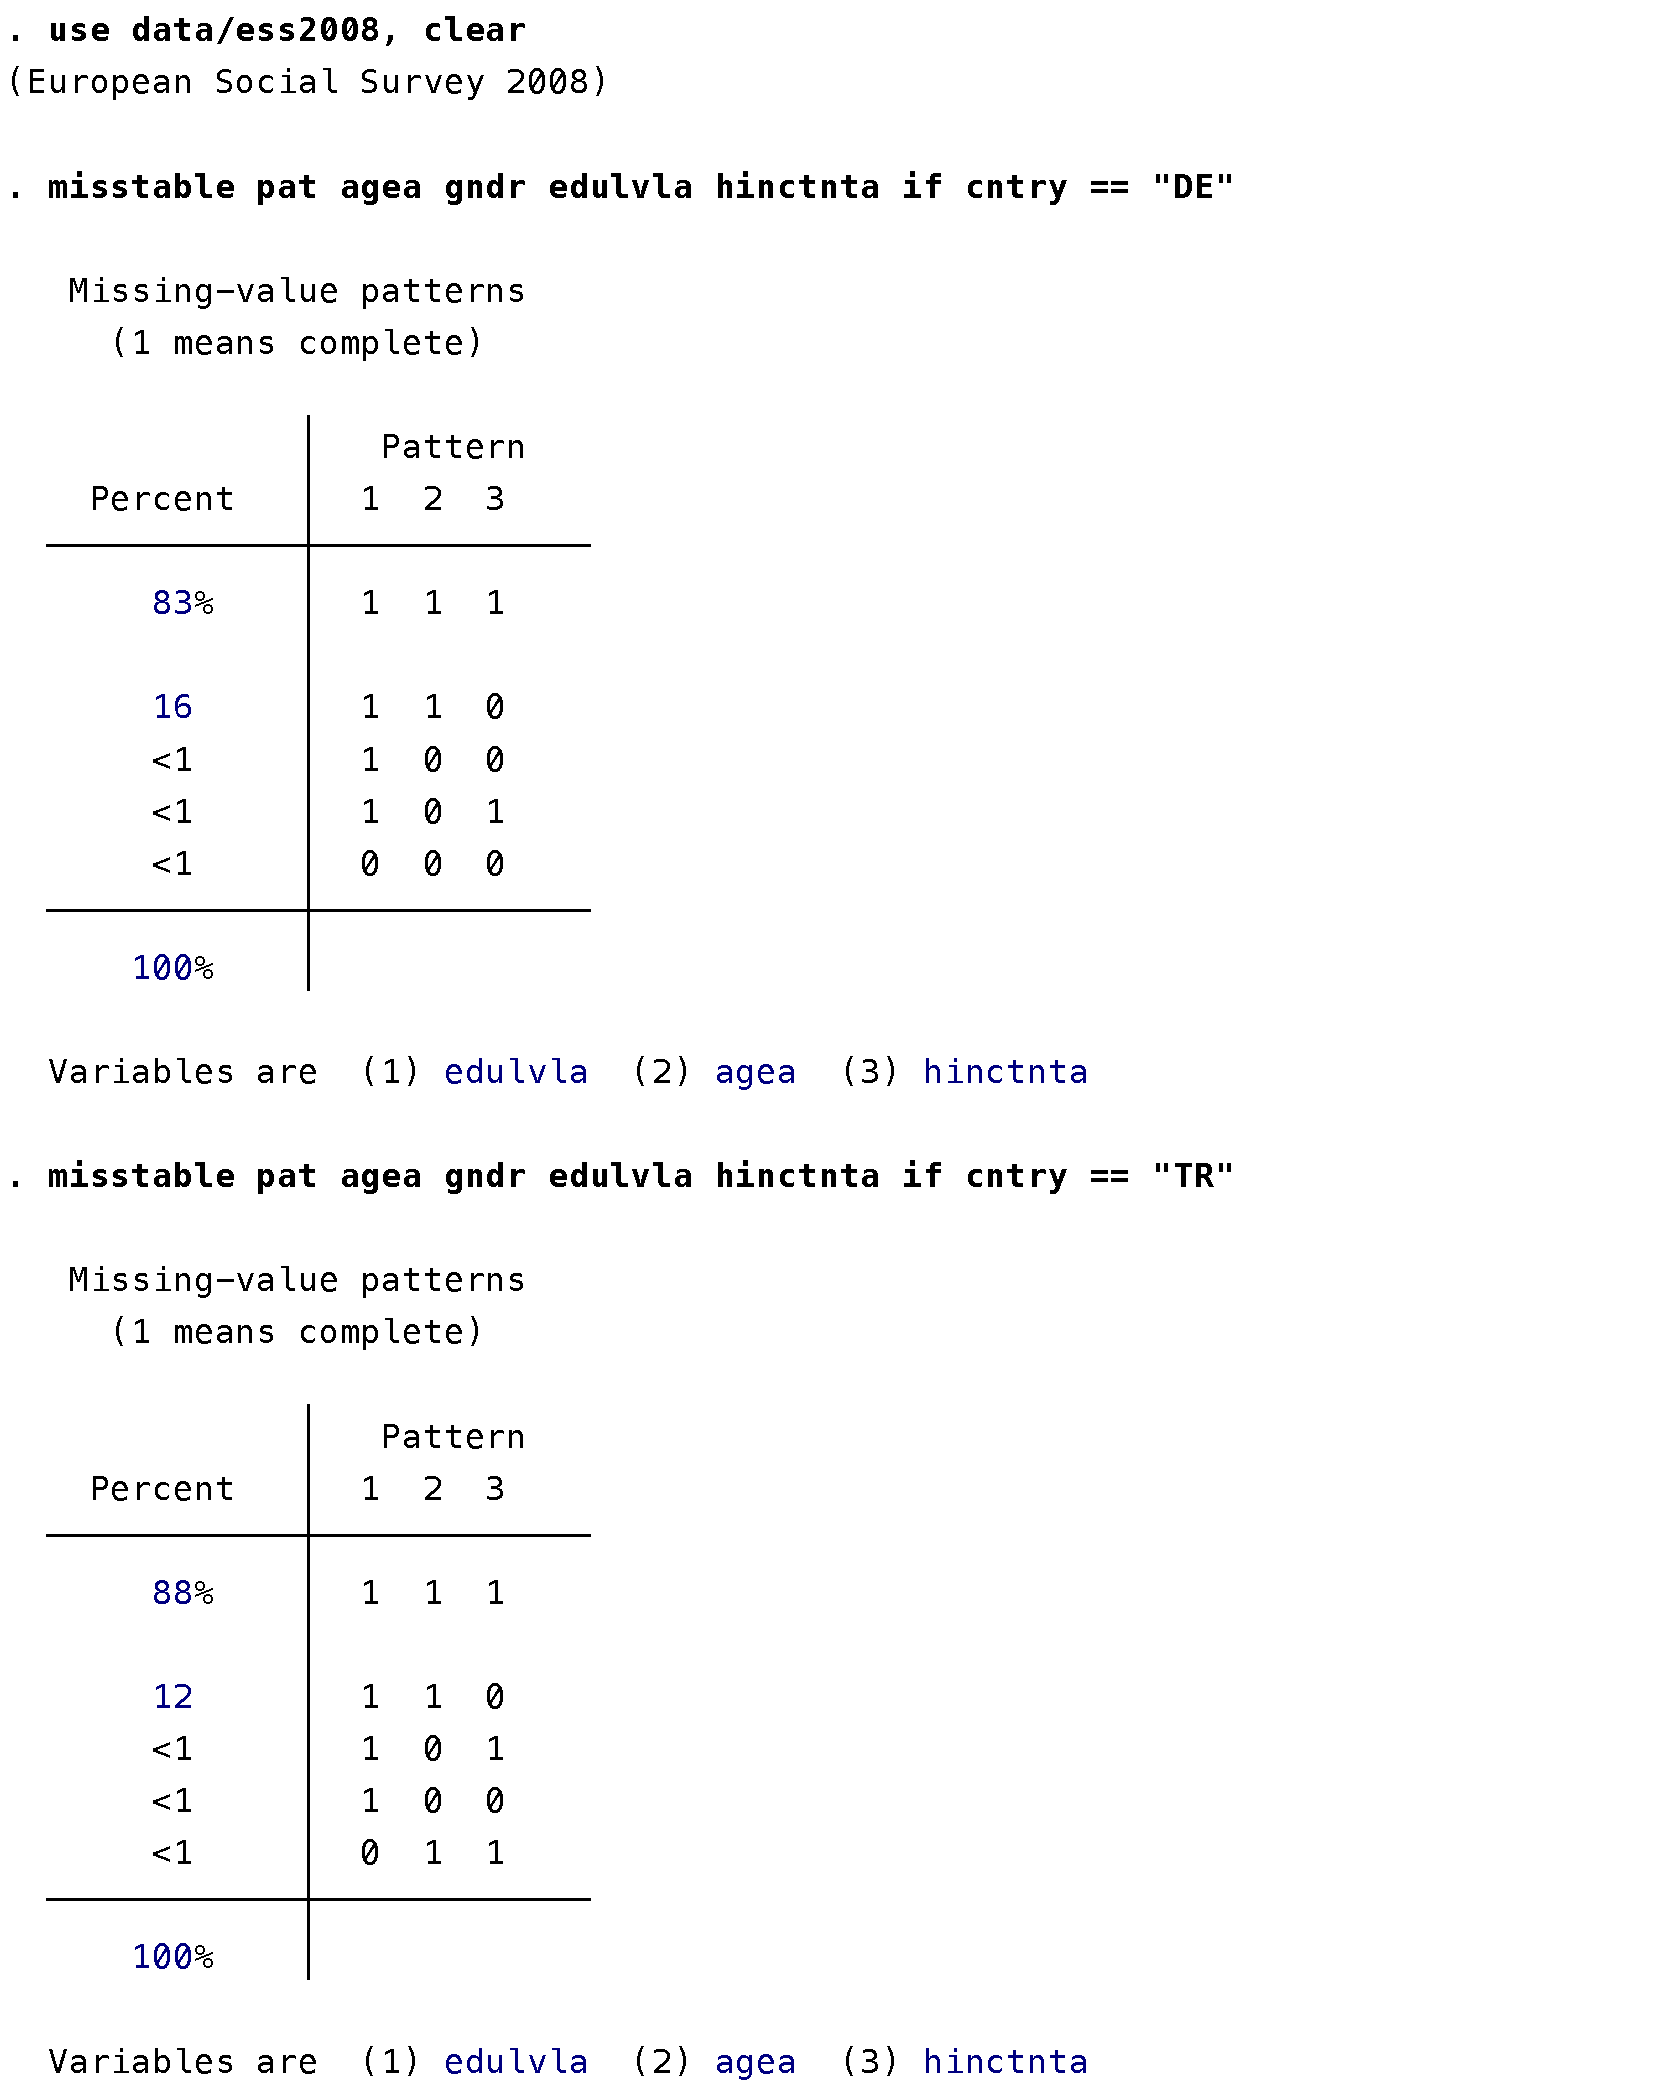
\includegraphics{ess-misstable-pat-cntry}\\[1em]
	
	Identically, on country-level data, you will also want to go a step further by inspecting the missing values more in depth. In this example, the \coab{freq}{frequency}{misstable} option shows the precise number of countries that would be left in the data with the following selection of variables:\\[1em]
	
	\begin{docspec}
		use data/qog2011, clear\\%
		* Missing values.\\%
		misstable pat wdi\_fr wdi\_gdpc bl\_asyt25 chga\_hinst\\[1em]%
		%
		* Missing values dummy.\\%
		gen missing = mi(wdi\_fr, wdi\_gdpc, bl\_asyt25, chga\_hinst)\\%
		* Geographic comparison.\\%
		table ht\_region, c(n missing mean missing)
	\end{docspec}
	
	The last lines of the code create the \texttt{missing} dummy equal, for each observation, to 1 if there is any missing data in the selected variables, and 0 otherwise. The mean of the dummy is then shown by geographical region, showing for instance that 93\% of the 29 East European and post-Soviet Union countries have missing data in the selected variables:\\[1em]
	
	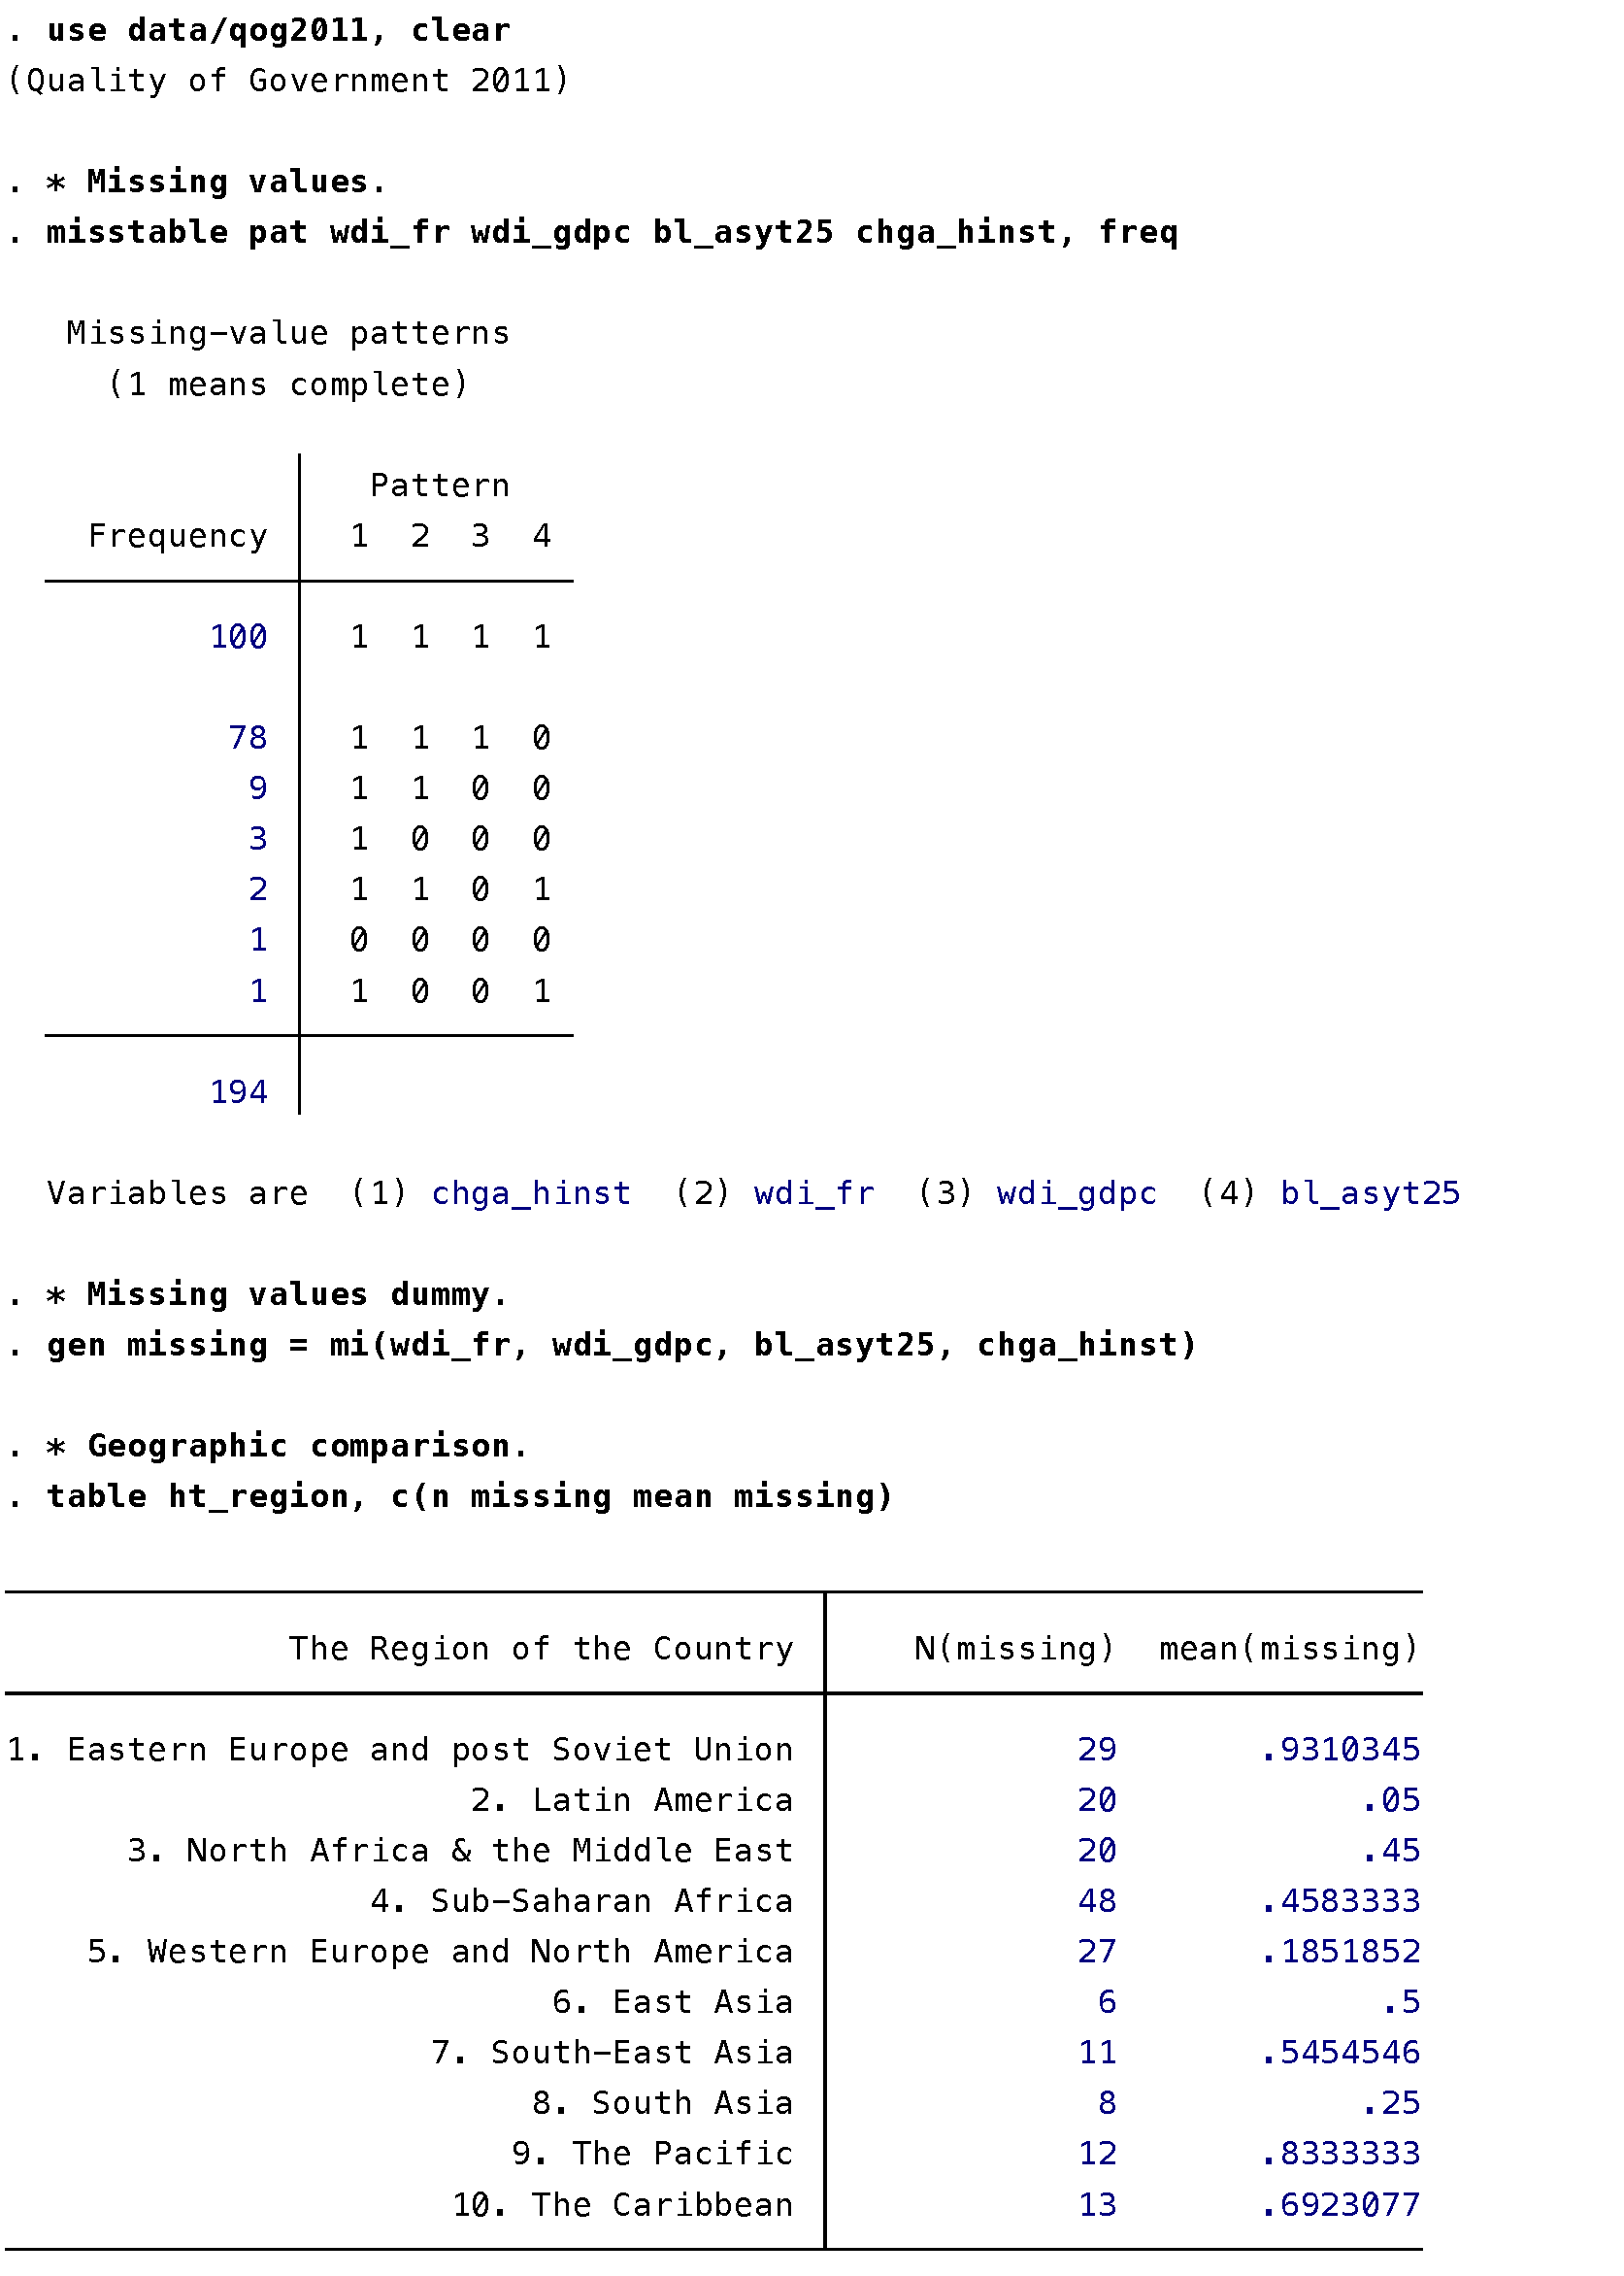
\includegraphics{qog-misstable-freq}\\[1em]
	
	\newthought{The amount of missing values in the data} becomes an issue when it starts affecting the representativeness of your sample, or when it simply falls too low for statistical tests to operate properly; the oft-cited threshold is around $N = 30$, but anything low is both a threat to external validity and a handicap for the subsequent analysis. 
	
	Your finalized sample is the sample left after subsetting to full data with the \cmd{drop} and \cmd{keep} commands. The example below subsets the \ESS data twice, first to keep only observations from two country case studies, then to delete observations with missing data:
	
	\begin{docspec}
		use data/ess2008, clear\\
		* Keep only Germany and Turkey.\\
		keep if inlist(cntry, "DE", "TR")\\
		* Remove missing data.\\
		drop if mi(agea, gndr, edulvla, hinctnta)
	\end{docspec}
	
	\newthought{What can be done about missing data} is a topic that goes beyond the scope of this class, into interpolating and, by extension, simulation. The conservative view that we adopt here for simplicity consists in recommending that the only cure for data is more data.

%% - missing values
%% misstable, drop, keep, count

%
%
% 1.3 ==========================================================================
%
\subsection{Categorical recodes}
\label{sec:categorical-recodes}

Recoding occurs when you alter the numeric structure of a variable. Your aim is generally not to alter the data itself, but rather to produce alternative classifications of it. The next paragraphs cover most common situations.

\begin{description}

	\item[Reverse-coding]% % % % % % % % %
	%
	Let's start with an example. In the General Social Survey, general happiness has been coded on a three-point scale that ranges from 1 ``Very happy'' to 3 ``Not too happy'': 

\begin{docspec}
	use data/gss2010, clear\\
	fre happy\\
\end{docspec}

The \cmd{fre} command is particularly useful here because it shows the basic structure of the variable (name, description, values and labels) along with its frequencies in just one short command:\\[1em]

	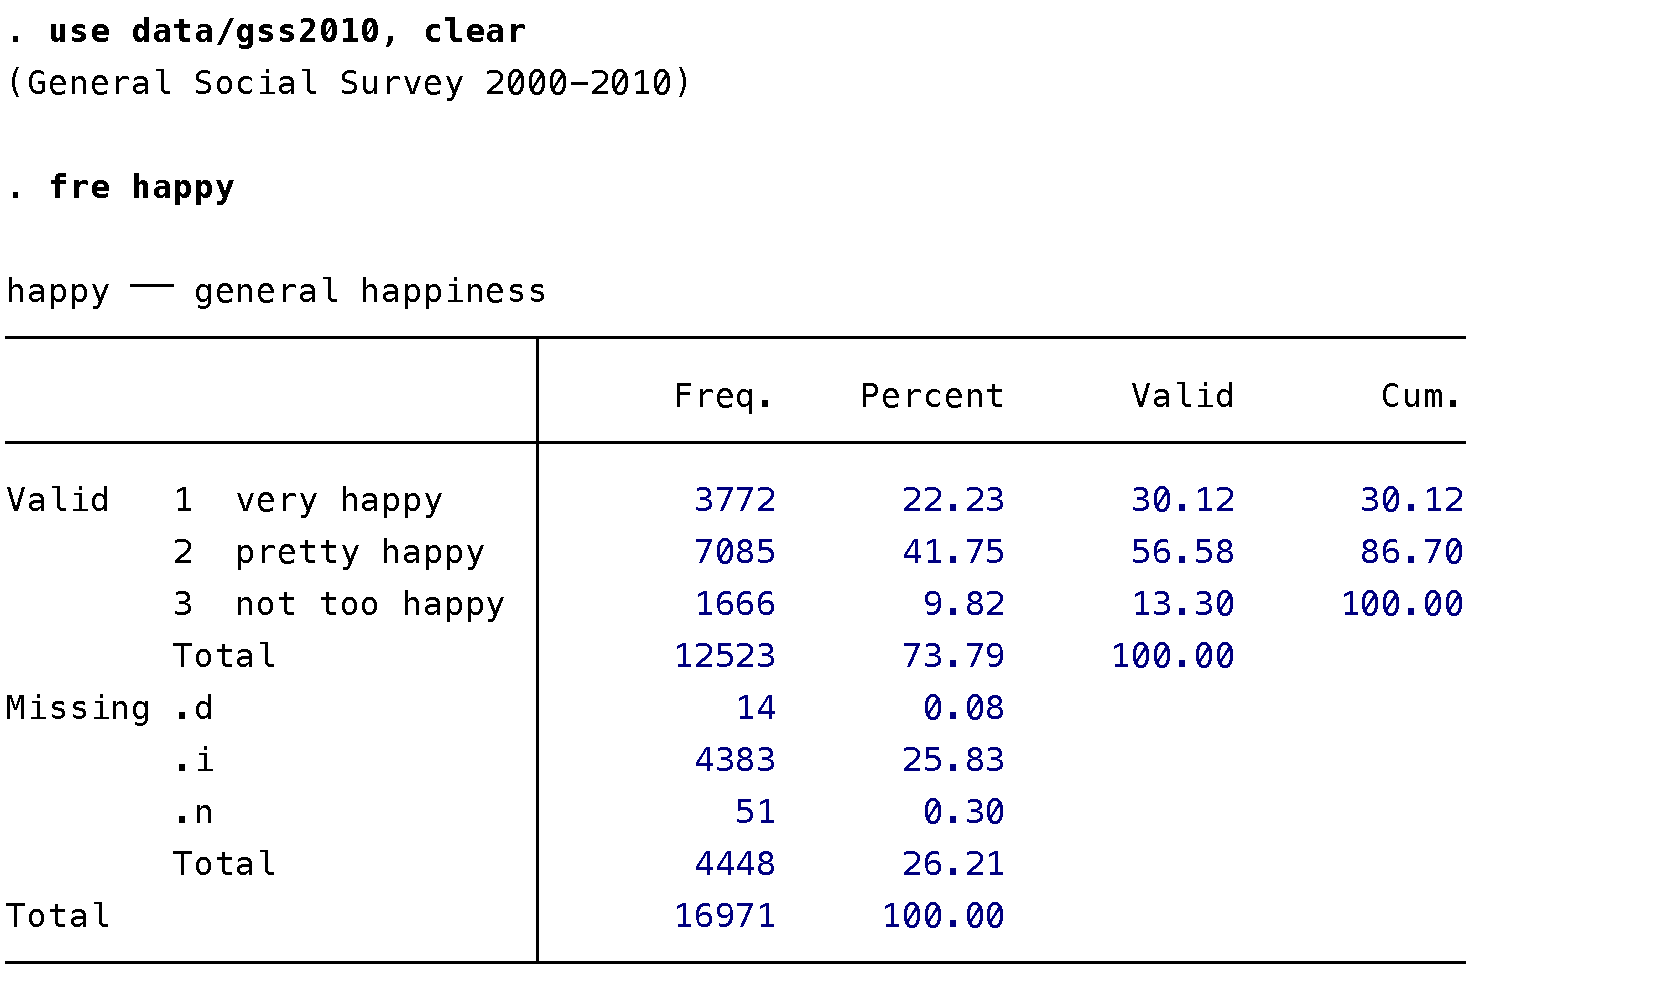
\includegraphics{gss-happiness}

The variable can be easily reversed to the opposite coding by substracting the scale to its maximum $+ 1$, and then by relabelling the values of the new variable:

\begin{fullwidth}
	\begin{docspec}
		gen happiness:happiness = 4 - happy\\
		la def happiness 1 "Not too happy" 2 "Pretty happy" 3 "Very happy", replace\\
		fre happiness
	\end{docspec}
\end{fullwidth}

In the example above, the \cmd[gen]{generate} command handles the numeric reverse by creating a new variable called \texttt{happiness}, for which a \emph{value label} is simultaneously defined under the same name. The label is then defined with the \cmd[la def]{label define} command, so that the new variable will show the same text labels than the original one:\\[1em]

	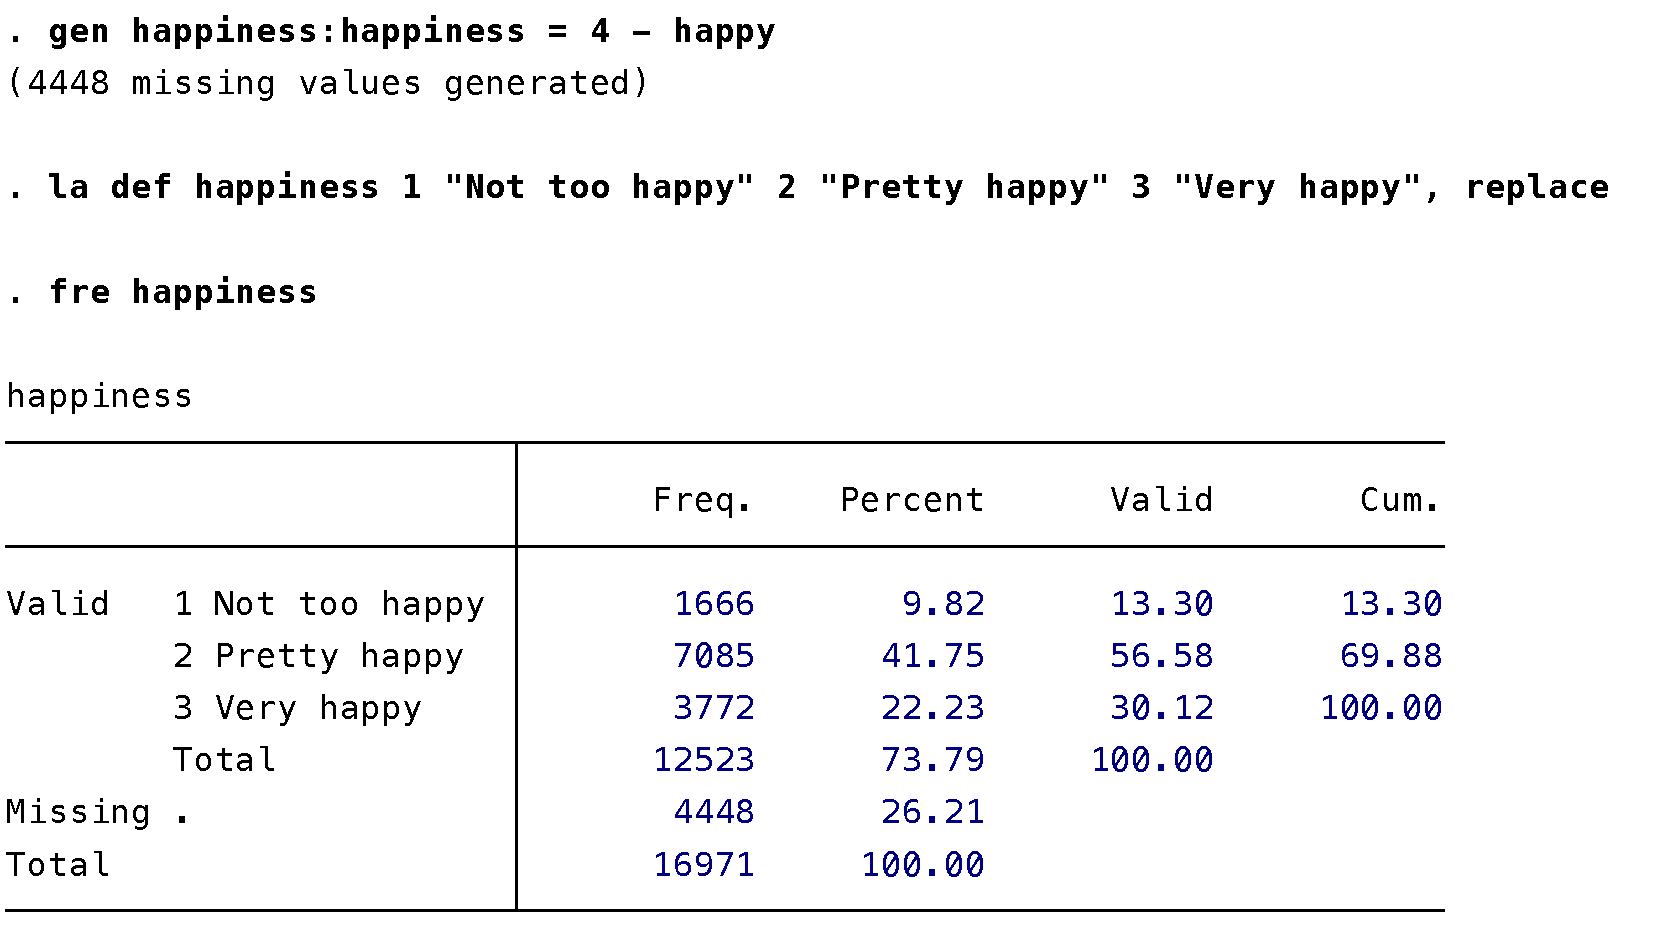
\includegraphics{gss-happiness-reverse-coding}\\[1em]

\index{Labels!For values}%
Stata syntax for value labels is pretty straightforward. The trick is to remember to assign the value label to the variable, or the labels will not show. This can be done through the \texttt{gen x:x} trick shown above, or through the \cmd[la val]{label values} command. One value label can be applied to any number of variables: a generic `yes/no' value label can therefore be applied to several variables at once.%
	\footnote{This system is not only convenient, it is also a way to compress the data.}
Type \texttt{h la} for further illustrations of value labels.

	\item[Recoding to less groups]% % % % % % % % %
	%
Another common situation is having to recode a categorical variable to less groups than it originally had, in order to create groups large enough for cross-tabulation and statistical testing. The next example shows an extract of the \ess, in which left-right positioning has been measured on an 11-point scale coded from 0 (extreme-left) to 11 (extreme-right):

\begin{docspec}
	use data/ess2008 if cntry == "HU", clear\\
	fre lrscale
\end{docspec}

The extract loads only the data for Hungary ($N = 1544$ respondents). We should consider recoding the scale to less precise but more populated categories, because the number of respondents at each level of the scale is often very low and threatens to provide too little statistical power:\\[1em]

	\includegraphics{ess-load-hungary-lrscale}\\[1em]

	\item[Recoding to intervals]% % % % % % % % %
	%

	\item[Recoding to dummies]% % % % % % % % %
	%
A specific case of recoding is when you are recoding to only two values, he female dummy recode from p.~\pageref{female-dummy} we have used a logical statement

	\item[Encoding a string variable]% % % % % % % % %
	%
	% encode
	
	\item[Replacing a string value]% % % % % % % % %
	%
	% replace
	
\end{description}%
%
%
% 2
%
\section{Additional data skills}
\label{sec:additional-data-skills}

% 2.1
%
\subsection{Converting datasets}
\label{sec:data-conversion}
\index{Data!Conversion}

% CSV
\label{sec:insheet}
\index{Data!Conversion!From \textsc{csv} files}

\newthought{Plain text files} that use \underline{c}omma-\underline{s}eparated \underline{v}alues (\ext{.csv}) can be imported into Stata if you carefully clean the file first from any additional element that is not part of the data itself.%

% Fixed format
\label{sec:infix}
\index{Data!Conversion!From fixed format}

\newthought{Fixed-format data} consists of variables that have been separated by a fixed number of spaces. This format is more complex to manipulate than delimited text, as you have to determine the precise format of the data and run extensive code to name variables and apply labels, using a `dictionary' file.%

Details on how to proceed with fixed-format data in Stata appear in the help page of the \cmd{infix} command, and short examples can be retrieved from online Stata tutorials. For an example with the National Health Interview Survey of 2009%
  \footnote{\url{http://www.cdc.gov/nchs/nhis/nhis_2009_data_release.htm}}, %
  you can try downloading and uncompressing one of the \textsc{ascii} data files for that year%
  \footnote{\eg \url{ftp://ftp.cdc.gov/pub/Health_Statistics/NCHS/Datasets/NHIS/2009/personsx.exe} (provided in self-extracting \textsc{exe} format)}, %
  and then apply the sample Stata statements provided by the data teams to see what is involved in producing the final dataset.%
  \footnote{\eg \url{ftp://ftp.cdc.gov/pub/Health_Statistics/NCHS/Program_Code/NHIS/2009/personsx.do}}%

If you try to process the example above, you will realize that fixed format data is difficult to manipulate. Unless you have a \emph{lot} of time on your hands to convert and debug the files, do not engage into complex data wrangling with fixed format data.%

% XLS
\label{sec:import-excel}
\index{Data!Conversion!From Excel files}

Microsoft Excel files (\ext{.xls}) are written in a proprietary spreadsheet format that can be imported into Stata~12 with the \cmd{import excel} command. Datasets written for \textsc{sas}, \textsc{spss} or other statistical software can be converted with Stat/Transfer,%
  \footnote{StataCorp recommends this solution: \url{http://www.stata.com/products/stat-transfer/}. Sciences Po has made Stat/Transfer available on its workstations.} %
  or with free software by using R with the \texttt{foreign} package to import and export the data.%
  \footnote{See the procedure at \url{http://www.statmethods.net/input/importingdata.html}. The \texttt{foreign} package is reliable but leaves some encoding issues.}%

As soon as you take it on yourself to convert the data rather than to trust the data team responsible for the original data files, you are exposing yourself to conversion errors and will almost certainly have to perform time-consuming verifications on your unofficial dataset.%

For this reason, your safest option is to use official data files provided in the Stata proprietary format, or to rely on a machine-readable format of your data like \ext{.csv} (comma-separated values) that can be read in any software.%

% 2.2
%
\subsection{Merging datasets}
\label{sec:merge}


%%%% WBOPENDATA
% \section{Accessing World Bank Open Data in Stata}
% http://data.worldbank.org/news/accessing-world-bank-open-data-in-stata

%%%% MERGING COUNTRY REGIONS AND STD NAMES WITH KOUNTRY


% 2.3
%
\subsection{Rescaling variables for indexes}

You can create indexes out of several variables with \emph{identical} ranges by adding or multiplying them, but when the variables have different ranges, you will need to standardize them on a common scale of measurement if you want to ensure that the resulting index takes each component equally into account.

Standardization is common in disciplines like demography and epidemiology, where mortality rates, for instance, have to be age-standardized to compare across time and space. Such operations typically require additional information about the general population.%
  \footnote{For a Stata tutorial, see \url{http://data.princeton.edu/eco572/std.html}}

The simplest standardized scale will consider the minimum value of the variable to be $0$ and its maximum to be $1$, and will express all other values as a fraction of the maximum, therefore creating a $0$--$1$ scale out of the variable.

\label{sec:gtsd01}%
Use the \cmd{std01} command for that purpose. If the command was not installed by the course setup, run this installation command:%
	
  \begin{fullwidth}
	  \begin{docspec}
		  net install \_gstd01,%
			  from(\url{http://web.missouri.edu/~kolenikovs/stata})
	  \end{docspec}  
  \end{fullwidth}
	
The command is an extension to the Stata \cmd{egen} command, and works as shown below, where we merge three \QOG variables on gender equality to a single \texttt{index} variable of range $0$--$3$:%

\begin{docspec}
	use data/qog2011, clear\\
	d wdi\_gris gid\_rfmi gid\_fptw\\
	egen gris01 = std01(wdi\_gris)\\
	egen rfmi01 = std01(gid\_rfmi)\\
	egen fptw01 = std01(gid\_fptw)\\
	gen index = gris01 + rfmi01 + fptw01
\end{docspec}

There is a fair chance, however, that the result of an index will not intuitively convey much information. It might also suffer from the different variability of each variable, regardless of the common scaling. Further diagnostics are generally in order at that stage, the main one being: what have you \emph{really} gained with an index?

Most of the time, making a decisive choice between two or more variables with meaningful units will indeed be a better idea than dropping both of them for a unit-less measure that comes with little guarantee of being balanced and therefore reliable.\footnote{That being said, I guess that the Society of Indexers would disagree: \url{https://rulesofreason.wordpress.com/2012/11/20/the-international-journal-of-indexing/}}%
%
% %
% 3
%
\section{Advanced data skills}

The following operations are \emph{not} covered in the course because they require extensive checks that would take too much time to process. You are strongly advised \emph{not} to try any of the operations below, unless you can allocate several additional working hours to your project in the first weeks of class.

% 3.1
%
\subsection{Cross-dataset pooled questions}

Some polling items are close enough in question wording to be pooled in order to increase sample size and/or periodicity. Some attitudinal surveys, including some used in the course datasets, also use common rotating modules to provide cross-national comparability. Pooling can introduce a vast range of issues that require sensitivity checks to ensure that the pooling does not create idiosyncratic effects, thereby threatening the validity of the data.

When done right, pooling can also correct for many issues rather than creating new ones. Electoral forecasts, which do not aim at explaining the determinants of an election but rather to extract the predicted score from pre-electoral polls, can use pooling to produce very precise models. The most recent example with remarkable accuracy was Nate Silver's `538' electoral forecast for the \emph{New York Times}, which perfectly predicted the electoral college of the U.S. presidential election of November 2012. The methodology is not entirely clear, but it rests on a lot of pooled time series data.%
\footnote{\url{http://fivethirtyeight.blogs.nytimes.com/methodology/}} %
Drew Linzer's \emph{Votamatic} model has a similar methodology and more details.%
\footnote{\url{http://votamatic.org/how-it-works/}}

% 3.2
%
\subsection{Reshaping and collapsing}

Time series data can come in two formats, depending on whether there is one row of observation per year (`wide' format) or several (`long' format). The \cmd{reshape} command can convert from one to the other format.
    
The course datasets are cross-sectional and do not require reshaping prior to analysis.

% 3.3
%
\subsection{Fixed-format data}

Fixed-format data consists of variables that have been separated by a fixed number of spaces. This format is more complex to manipulate, as you have to determine the precise format of the data and run extensive code to name variables and apply labels, sometimes using a `dictionary' file.
    
Details on how to proceed with fixed-format data in Stata appear in the help page of the \cmd{infix} command, and short examples can be retrieved from online Stata tutorials.
    
For an example with the National Health Interview Survey of 2009%
\footnote{\url{http://www.cdc.gov/nchs/nhis/nhis_2009_data_release.htm}}, %
you can try downloading and uncompressing one of the \textsc{ascii} data files for that year%
\footnote{e.g. \url{ftp://ftp.cdc.gov/pub/Health_Statistics/NCHS/Datasets/NHIS/2009/personsx.exe} (provided in self-extracting \textsc{exe} format)}, %
and then apply the sample Stata statements provided by the data teams to see what is involved in producing the final dataset.%
\footnote{e.g. \url{ftp://ftp.cdc.gov/pub/Health_Statistics/NCHS/Program_Code/NHIS/2009/personsx.do}}
    
    If you try to process the example above, you will realize that fixed format data is difficult to manipulate. %
    Unless you have a \emph{lot} of time on your hands to convert and debug the files, do not engage into complex data wrangling with fixed format data.

% coda:

Last, datasets produced for \textsc{sas}, \textsc{spss} or other statistical software can be converted to Stata using the Stat/Transfer software.%
  \footnote{\url{http://www.stattransfer.com/}} %
StataCorp itself recommends the software,%
  \footnote{\url{http://www.stata.com/products/stat-transfer/}} %
and Sciences Po has made it available on its microlab workstations.

A free alternative consists in using the R statistical software with the \texttt{foreign} and \texttt{Hmisc} libraries to import the data in R and then export it to Stata.%
  \footnote{\url{http://www.statmethods.net/input/importingdata.html}} %
There is absolutely no guarantee, however, that the conversion process will be error-free.

In both cases, if you are taking it on yourself to convert the data rather than to trust the data team responsible for the original data files, then you are exposing yourself to conversion errors and will have to perform time-consuming verifications on your unofficial dataset.

For these reasons, your safest option is either to use official data files provided in the Stata proprietary dataset, or to rely on a machine-readable format like \textsc{csv} to be able to open the file from any software.
%
%

\stopcontents[chapters]

%
% have a nice day
%
        %% ... sessions 2-3 (data, vars)
  \chapter{Distributions}%
	\label{ch:distr}%
	\index{Distributions}%
	%
	%

%% -- a few words

\minitoc
%
\newpage
%
%

%
%
%
\section{Descriptive statistics}

	%
	% 2.1.1
	%
	\subsection{Measures of central tendency}

	%
	% 2.1.2
	%
	\subsection{Dispersion around the mean}

	%
	% 2.1.3
	%
	\subsection{Exporting descriptive tables}

%
%
%
%
%
\section{Visualizing distributions}

	%
	% 2.2.1
	%
	\subsection{Faceting: plotting over small multiples}

	%
	% 2.2.2
	%
	\subsection{Quantiles: plotting an empirical distributions}

	%
	% 2.2.3
	%
	\subsection{Normality: plotting a probability distribution}

%
%
%
%
%
\section{Instructions for the first draft}%
  %
  %
  \label{sec:draft1}%
  %
  %
  \index{Coursework!Research project!First draft}%
  %
  %

% The course is built around your elaboration of a small-scale research project. Because the course is introductory by nature, several limits apply:
% 
% −	You are required to use pre-existing data, instead of assembling your own data and building your own dataset, which is a much longer process that require ad-ditional skills in data manipulation.
% −	You are required to use cross-sectional data, because time series, panel and longitudinal data require more complex analytical procedures that are not cov-ered in introductory courses.
% −	You are required to use continuous data, because discrete variables also use different techniques not covered at length in the course. This applies principally to your choice of dependent variable.
% 
% These requirements and their terminology are covered in Section 5. For now, just re-member this basic principle: your research will be based on one dependent variable, sometimes called the `response'' variable, and you will try to explain this variable by predicting the different values that it takes in your sample (dataset) by using several independent variables, sometimes called the `explanatory'' variables, or `predictors'', or `regressors'' in technical papers.
% 
% Because your research is a personal project, you might bend the above rules to some extent if you quickly show the instructors that you can handle additional work with da-ta management. The following advice might then apply: 
% 
% −	If you are assembling your data by merging data from several datasets, you will be using the merge command in Stata (Section 5.2). You might also choose to use Microsoft Excel for quicker data manipulation. Do not assemble data if you do not already have some experience in that domain.
% −	If you are converting your data, refer to the course and online documentation on how to import CSV data into Stata using the insheet command, or how to convert file formats like SAV files for SPSS. Always perform extensive checks to make sure that your data were properly converted into a readable, valid file.
% −	If you are interested in temporal comparison, such as economic performance before and after EU accession, you can compute a variable that will capture, for example, the change in average disposable income over ten years. Stick with a single variable, and ask for advice in class before proceeding.
% −	If you have selected nominal data as your dependent variable, such as religious denomination, then something went wrong in your research design—unless you know about multinomial logit, in which case you should skip this class. Please identify a different variable that is either continuous or `pseudo-continuous''—i.e. a categorical variable with an ordinal (or better, interval) scale, such as edu-cational attainment.

	\subsection{Dataset selection}

%% from the README file of the data folder:

% Open each dataset with the `use` commands provided in this document. These require that the `SRQM` folder has been set as the working directory, as explained in its [README][srqm-readme] file. Then use the `lookfor` and `lookfor_all` commands to explore the variables. Finally, select one dataset and make a selection of variables relevant to your research project.
% 
% Bibliographic information and additional documentation is available from the online data sources. Once you have identified a dataset, retrieve that information to describe its sampling and weighting design. Include a full reference to the data in your paper, including author names, release year, version number and URL to the data website.
% 
% Indications on weighting the data with the `svyset` command are provided for point estimation. It is unlikely that you will need to do that yourself, but you should include the weighting scheme in your do-file for reference. Place it right after opening the data with the `use` command mentioned above.
% 
% Every single minute that you spend learning about your data by reading the documentation and exploring the variables is a minute well spent. It takes several hours to become sufficiently familiar with any complex data source. Finding and skim-reading a few papers that use the data is good practice.

	\subsection{Variable selection}

% /* Notes on selecting variables for analysis:
% 
%  - The first and most important choice is the dependent variable (DV), which has
%    to be a continuous variable, that is, a variable that takes many intervalled
%    values on a given scale. You must fully understand that aspect of the DV.
% 
%  - Some limitation in continuity is acceptable. The example provided here is a 
%    borderline case, as the DV is measured on a 5-point scale that makes it more 
%    categorical than continuous.
%    
%  - The reliability of your final analysis will be either more limited or more
%    complex if you choose a dependent variable that is less continuous than it is
%    categorical. There will be one late session on logistic regression for these.
% 
%  - Practical consequences: use either country-level data from the Quality of
%    Government dataset, or use variables from the ESS, GSS and WVS surveys that
%    were measured on 7-pt or 10-pt scales, or something even higher than that.
% 
%  - You can violate that recommendation in two cases:
%  
%    (1) You are interested in having a particular categorical variable as your
%        dependent variable, and you are willing to go one extra mile in the late
%        stage of this course by learning additional modelling.
%    
%    (2) You have found a categorical variable that is pseudo-continuous, i.e.
%        that follows some approximation of the normal distribution. We will cover
%        the normal distribution next week, so stay tuned.
% 
%    In either case, you will have to proceed cautiously. The main skill here is
%    the ability to understand the structure of your data, as you would in other
%    research situations that rely on different forms of research material.
% 

%  - The next step is to select independent variables (IVs). Some of them will 
%    work as controls: you want to make sure that you understand how your DV
%    relates to persistent, structural factors that are hard to affect altogether.
% 
%  - Some other independent variables will operate as DV predictors: you want to
%    test the idea that your DV is determined by these IVs, by showing that the
%    values taken by these IVs can predict those taken by the DV.
% 
%  - Finally, some independent variables might be more covariates than predictors,
%    i.e. variables that you predict to be strongly associated to the DV and to
%    vary in related directions (as with "the higher..., the lower...").
% 
%  - If you are going to work with survey (individual-level) data, include common
%    socio-demographics like age, sex, education, household composition, e.g.
%    marital status and number of children (and possibly household income).
%    
%  - If you are going to work on country-level data, include at least one variable
%    for economic development (the most common measure is GDP per capita) and one
%    measure of political organization (e.g. democratic v. dictatorial regime). 
%  
%  - Quickly check a few academic references on your topic to see what variables
%    might be relevant. The course contains a few example papers, and other ones
%    are easy to locate using Google Scholar with precise keywords. */

	% missing values, recodes, summary stats
%
%
       %% ... sessions 4-5 (summ, distr) ... ends on: draft 1
  
  % 2) hyp tests
  % 
  \chapter{Significance}%
	\label{ch:sig}%
	\index{Significance (statistical)}

% illustrated with this:
% http://montclairsoci.blogspot.ch/2012/07/bitter-tea.html

	\newthought{A hypothesis} is a statement that you can either confirm or contradict. ``People at the extremes are happier than political moderates \dots none, it seems, are happier than the Tea Partiers \dots'', for instance, is a verifiable statement that happens to be false in the context in which it was formulated.\footnote{The statement is from a \emph{New York Times} article by Arthur Brooks. See Jay Livingston's blog, ``\href{http://montclairsoci.blogspot.ch/2012/07/bitter-tea.html}{Bitter Tea?}'' (10 July 2012), and Andrew Gelman's blog, ``\href{http://andrewgelman.com/2012/08/1-5-million-people-were-told-that-extreme-conservatives-are-happier-than-political-moderates-approximately-0001-million-americans-learned-that-the-opposite-is-true/}{1.5 million people were told that extreme conservatives are happier than political moderates. Approximately .0001 million Americans learned that the opposite is true}'' (14 August 2012).} You can verify this yourself by looking into the U.S. General Social Survey from 2010:%

	\begin{verbatim}
	use datasets/gss2010, clear
	spineplot happy partyid if partyid < 7 [aw=wtssall], ///
	    xla(, alt axis(2)) xti("", axis(2)) scheme(set1)
	\end{verbatim}

The \cmd{spineplot} command above displays proportions of the sample by level of subjective happiness (\texttt{happy}) and political party affiliation (\texttt{partyid}, with over 97\% of the respondents placing themselves on a scale ranging from 0 ``Strong Democrat'' to 6 ``Strong Republican''). The graph options on the last line are optional.

The result visually contradicts the previous statement by suggesting a more ambiguous relationship between the two variables:

\begin{figure}
    \includegraphics{gss-happy}
    \caption[Subjective happiness by political affiliation.]%
    {Subjective happiness by political affiliation. %
    \emph{The General Social Survey, which started in 1972, has repeatedly measured both variables over the years. The pattern suggested by Arthur Brooks holds when the data are averaged over the years, but it visibly does not hold for 2010.}}%
    \label{fig:stata-window}
\end{figure}

\newthought{Hypothesis testing} is a way to test your data against a hypothesis. Statistical significance tests do so by assuming that you want to compare your data against randomness, in order to prove that the associations you observe in the data are very unlikely to be due to an accidental sampling error. The `hypothesis' in `hypothesis testing' is therefore the possibility of an association in the data being random. This is denoted $H_0$ and called the \emph{null hypothesis}.

More generally, the null hypothesis assesses something like this:

\begin{quote}
	If the data were generated randomly, how likely is it that we would obtain a pattern identical to the one that we observe in the sample?
\end{quote}

\newthought{Rejecting the null hypothesis} involves specifying what the null hypothesis might be. If you are inspecting income by gender, it might be that the average income is lower among females than among males. If you are exploring party affiliation and subjective well-being, it might simply be the existence of an association between the two variables. 

Intuitively, your \emph{substantive} hypothesis is that an association or a difference \emph{does} exist in the data. Statistics do not take over your hypothesis, and instead offer you the possibility to prove it by contradiction, by rejecting the null hypothesis of an accidental association that could also exist in randomly generated data.

\newthought{Statistical significance} characterizes an association for which the null hypothesis is highly unlikely. The common 95\% and 99\% levels of confidence are conventional thresholds at which you can choose to reject the null hypothesis. At these thresholds, the probability of the null hypothesis is respectively $p < .05$ and $p < .01$.\footnote{The probability of the null hypothesis $H_0$ is called the $p$-value and the level of statistical significance at which you reject $H_0$ is called $\alpha$.}

\newthought{Be careful:} the probability of your substantive hypothesis, denoted $H_a$ for ``alternative hypothesis'', is \emph{not} equal to $1 - p$. The low probability that there is no association \emph{at all} in the data does not mean that your specific hypothesis on that association is correct.

Take, for instance, this abstract from a U.S. libertarian think tank (emphasis added):

\begin{quote}
	A number of theorists assume that drinking has harmful economic effects, but data show that drinking and earnings are positively correlated. \textbf{We hypothesize that drinking leads to higher earnings by increasing social capital.} If drinkers have larger social networks, their earnings should increase. Examining the General Social Survey, we find that self-reported drinkers earn 10-14 percent more than abstainers, which replicates results from other data sets. We then attempt to differentiate between social and nonsocial drinking by comparing the earnings of those who frequent bars at least once per month and those who do not. We find that males who frequent bars at least once per month earn an additional 7 percent on top of the 10 percent drinkers' premium. These results suggest that social drinking leads to increased social capital.\footnote{The abstract is from a Reason Foundation report by Bethany L. Peters and Edward Stringham, ``\href{http://reason.org/news/show/127594.html}{No Booze? You May Lose. Why Drinkers Earn More Money Than Nondrinkers}'' (September 2006).}
\end{quote}

In this study, if the null hypothesis $H_0$ is the absence of any association between earnings and drinking, then the presence of a relationship is hardly surprising. However, the probability of that relationship is \emph{not} equal to the probability of the alternative hypothesis $H_a$ stating that ``drinking leads to higher earnings'', as the reverse statement might also be true to some (possibly wider) extent.\footnote{Devise at least two reasons why the causality might run from high income to frequent social drinking, rather than vice versa. I owe this question and example to \href{https://pinboard.in/u:cshalizi/b:d54b8c984beb}{Cosma Shalizi}.}

\newthought{Furthermore,} rejecting the null hypothesis while it is actually true, or the reverse error, is still a possible outcome of your interpretation of the test. 

\newthought{Statistical significance has no effect on bias.} If your sample, measurements or hypotheses are biased, or if your reporting of their tests is, then you are left with an entirely different set of issues to deal with. The problem is ubiquitous among all branches of contemporary science:

\begin{quote}
	There is increasing concern that most current published research findings are false. The probability that a research claim is true may depend on study power and bias, the number of other studies on the same question, and, importantly, the ratio of true to no relationships among the relationships probed in each scientific field. In this framework, a research finding is less likely to be true when the studies conducted in a field are smaller; when effect sizes are smaller; when there is a greater number and lesser preselection of tested relationships; where there is greater flexibility in designs, definitions, outcomes, and analytical modes; when there is greater financial and other interest and prejudice; and when more teams are involved in a scientific field in chase of statistical significance\cite{Ioannidis:2005u}.
\end{quote}

To minimize bias, first make sure that you fully understand the limitations of your dataset and variables. Then, make sure that you formulate your hypotheses in the clearest possible way. Finally, report both negative and positive findings for which you have both a statistical significance test and some observation to substantiate its result.


%
%
%
\section{Confidence intervals}

	%
	% 4.1.1
	%
	\subsection{Applying the ``CLT''}

	%
	% 4.1.2
	%
	\subsection{Estimating a ``95\% CI''}
%
%
%
%
%
\section{Significance tests}

	%
	% 4.2.1
	%
	\subsection{Comparing two means}

	%
	% 4.2.2
	%
	\subsection{Comparing two proportions}
%
%
%
%
%
\section{Crosstabulations}

	%
	% 4.3.1
	%
	\subsection{Chi-squared test}

	%
	% 4.3.2
	%
	\subsection{Odds ratios}
%
%
         %% ... sessions 6-7 (ci, ttest)
  %
% 5
%
\chapter{Least squares}%
  %
  %
  \label{ch:ols}%
	\index{Least squares}%
  %
  \begin{mybox}
    %
    \smallcaps{This section} deals with least squares. By the end of that section, you will submit the revised draft of your research project.%
    %
    \paragraph{Coursework} %
    This section is covered in class during Weeks~7--9. Make sure that you have fully replicated the course do-files for these weeks by the end of this section. Read  \citeauthor[ch.~8 and 13]{Urdan:2010a}, and optionally \citeauthor[ch.~3--4]{FeinsteinThomas:2002d}.%
    %
  \end{mybox}\\[4em]%
  %
  \startcontents[chapters]%
  \printcontents[chapters]{l}{1}{\setcounter{tocdepth}{2}}%
	%
	\newpage
	%

\newthought{Simple linear regression} is a configuration of events where you have only two continuous variables at hand.%

\newthought{This section} covers correlation and the ``ordinary'' least squares estimator for a bivariate relationship.%

%
%
%
\section{Correlation}%
  \index{Correlation}%
  \label{sec:correlation}

Correlation is the most straightforward way to visualize, measure and estimate linear dependence between two continuous variables, by looking for a pattern in their \emph{covariance}. Stata lets you build \emph{correlation matrixes}, from which you can read \emph{correlation coefficients} for any number of variables. Correlations can be partial or `semi-partial' and can be computed onto different subsamples, depending on the exact requirements of your analysis.%

Visual inspection of your data is almost always your first step to any serious analysis, and correlation is no exception. Your starting point will be scatterplots with tentative linear fits. What you will be looking for are visual associations between pairs of variables for which there are theoretical grounds to consider that they might be \emph{correlates}.%

You will then build a correlation matrix in order to detect multiple linear codependence, which is also called \emph{multicollinearity}, among your continuous variables. Multicollinearity might require that you amend your selection of model variables, in accordance with your theoretical intuitions and research design. This process is iterative, and implies that you move back and forth between your data and your research hypotheses.%

% linear dependence, Pearson correlation

	%
	% 5.1.1
	%
  \subsection{Visualizing correlates}%
    \index{Correlation!Visualizing correlates}

  \begin{figure}
    \begin{center}
      \includegraphics[width=0.48\textwidth]{images/abortion_sc_means.pdf}
    \end{center}
    	\caption[Linear correlation]{\label{fig:correlation_scatterplot}%
  	Scatterplot of support for abortion and mass education. %
    \qog}
  \end{figure}%

  Figure~\ref{fig:correlation_scatterplot} provides an example of a visual relationship to which linear regression might apply, between public opinion support for abortion and average schooling years at the population level. The visual relationship that you might detect in the data is typical of a linear \emph{correlation}. The average values of each variable are displayed on the graph to show how the data distribute around them: mostly in the bottom-left and top-right quadrants, which define a \emph{positive} linear correlation.%

  The relationships that your model will capture will be \emph{linear} ones. If you detect a quadratic or exponential relationship, correlation and regression will fail to reflect them adequately. Variable transformations can be used to circumvent this issue, but some curvilinear phenomena might persist in the data, in which case you should acknowledge this limitation in your reports.\footnote{Section~[9] covers usual variable transformations, available through the \cmd{ladder} and \cmd{gladder} commands in Stata. Ideally, your data might also justify selecting a non-linear model, as in the case of a log-linear relationship.}% \ref{sec:transformations}	

  Figure~\ref{fig:correlation_variance} offers a more detailed visualization of the variance in each variable. Recall the formulae from Section~[9] for the variance $\sigma^2$ and standard deviation $\sigma$ of a variable $X$: % ~\ref{sec:dispersion}

  $$\sigma^2_X = \text{Var}[X] = \frac{\sum (X_i - \bar X)^2}{N} \quad \text{and} \quad \sigma_X = \text{SD}_X = \sqrt{Var[X]} = \frac{\sum (X_i - \bar X)}{\sqrt{N}}$$%

  The calculation of variance involves squaring the sum of deviations between each value $X_i$ and the mean value of the distribution $\bar X$, which is then divided by the total number of observations $N$. The squared term serves to cancel out the fact that some of these deviations are positive ($X_i - \bar X > 0$), while others are negative ($X_i - \bar X < 0$).%

  Take a quick look at how support for abortion and mass education vary around their mean values in the sample:

  \begin{figure}[htp]
  	\centering
  	\includegraphics[width=.48\textwidth]{images/abortion_sc_yvariance.pdf}
  	\includegraphics[width=.48\textwidth]{images/abortion_sc_xvariance.pdf}

  	\caption[Variance in two variables]{\label{fig:correlation_variance}%
  	Scatterplots of support for abortion and mass education. %
    Negative variance in solid lines, positive variance in dashed lines. %
    \qog}
  \end{figure}%

  What the graphs show at that stage is a clear association in the deviations from the mean: for the values of mass education that are \emph{above} its average level, the level of support for abortion is also \emph{above} its average level, and reversely, at levels of mass education that are \emph{below} its sample mean, support for abortion also tends to fall \emph{below} its sample mean.%

  This association is grounded in the joint variance of the two variables and can be measured as their correlation coefficient. Identically, regression relies on the joint variance of the variables included in the model to estimate its own coefficients. Both require, however, some preliminary graphical check to confirm that their relationship is effectively linear.%

Figure~\ref{fig:grmat} shows another form of correlation matrix, obtained from the \cmd{gr mat}{graph matrix} (\texttt{graph matrix}) that uses scatterplots to show every possible correlation between the variables. The matrix takes a bit of time to display, but is indispensable in any serious analysis of covariance and detection of linear relationships between \emph{all} variables included in your model. 

\begin{figure}[htp]
	\centering
	\includegraphics[width=.9\textwidth]{images/abortion_grmat.pdf}

	\caption[Scatterplot matrix with \cmd{gr mat}]{\label{fig:grmat}
	Scatterplot matrix produced with \texttt{gr mat}. \qog}
\end{figure}%

The scatterplot matrix is susceptible to confirm that several independent variables are moderately or strongly correlated, which creates \emph{interactions} within your model. The linear relationships that occur in parallel to your model create an issue called \emph{multicollinearity}, especially if you fall for the common flaw of including tons of independent variables and end up with a `kitchen-sink' model.\cite{Schrodt:2011a} Section~\ref{sec:interactions} covers this issue in detail.

At that stage, you should have obtained enough information from correlation analysis to select variables and draft your model. Correlation measures are only bivariate measures of association and can be unreliable, especially on a low number of observations: Pearson's $\rho$, for instance, requires normally distributed data to stay efficient when $N$ falls below approximately 30 observations. However, correlation is appropriate for exploratory purposes, to refine your intuitions and hypotheses before you start estimating regression models.

	%
	% 5.1.2
	%
  \index{Correlation!Coefficients}\index{Pearson's $\rho$|{Correlation}}%
  \subsection{Correlation coefficients: Pearson's $\rho$}

  Correlation is a proxy for the statistical property of \emph{linear dependence} between two variables $X$ and $Y$, which we assume when we model $Y$ as a function of $X$.\footnote{Mathematically speaking, correlation is only a proxy for linear dependence because the two notions are not strictly equivalent: two variables $X$ and $Y$ can be uncorrelated without being independent (as is actually common). Similarly, $Y$ could be expressed as a function of $X$ even if the two variables are uncorrelated, but this function would systematically fail to predict any of the variance in $Y$ from the variance in $X$. Feel free to have a drink.} Correlation can be expressed as a single coefficient $\rho (X,Y)$ that varies from perfect negative correlation when $\rho = -1$ to perfect positive correlation when $\rho = +1$. A correlation coefficient of $\rho = 0$ indicates that the variables are uncorrelated.

  Figure~\ref{fig:correlation_examples} shows example distributions for the three `extreme' situations of perfect positive, perfect negative and quasi-null correlation in random data.

  \begin{figure}[htp]
  	\centering
  	\includegraphics[width=.32\textwidth]{images/correlate_pos.pdf}
  	\includegraphics[width=.32\textwidth]{images/correlate_neg.pdf}
  	\includegraphics[width=.32\textwidth]{images/correlate_rnd.pdf}

  	\caption[`Extreme' correlation coefficients]{\label{fig:correlation_examples}%
  	`Extreme' correlation coefficients: from left to right, %
    $\rho = +1$, $\rho = -1$ and $\rho \approx 0$. %
    Simulated from random data.}
  \end{figure}%

  The formula that is generally used for measuring correlation is Pearson's $\rho$, a coefficient measure that divides the \emph{covariance} of $X$ and $Y$ by the product of their standard deviations $\sigma_X$ and $\sigma_Y$, which are themselves the square roots of the variance in $X$ and $Y$:

  $$\text{Cov}[X,Y] = \frac{\sum{(X_i-\bar X_i)(Y_i-\bar Y_i)}}{N} \quad \text{and} \quad \rho_{X,Y} = \text{corr}[X] = \frac{\text{Cov}[X,Y]}{\sigma_X \sigma_Y} = \frac{\text{Cov}[X,Y]}{\sqrt{\text{Var}[X] \text{Var}[Y]}}$$

  Pearson's $\rho$ is calculated out of the sample estimates that we hold for the means $\bar X$ and $\bar Y$, which we write $\mu_X$ and $\mu_Y$ at the level of the population, or universe, from which we have sampled our data. Identically, Pearson's $\rho$ depends on the standard deviation of each variable in the sample, which we denote as $s_X$ and $s_Y$ for their sample values. Since it relies on estimated parameters, the correlation coefficient can be tested for statistical significance, in order to verify that it is different from $(H_0): \rho = 0$ at a given level of confidence.

  Stata offers two different commands for correlation with Pearson's $\rho$, both very straightforward. 

\subsection{Exporting correlation matrixes}%
  \index{Correlation!Matrixes}%
  \index{Correlation!Exporting results}

When you are done with visual inspection with scatterplots (\texttt{sc}), compute correlation coefficients for your selection of variables with the \cmd{pwcorr} command. The \texttt{pw} prefix in the name of the command stands for \emph{pairwise} case deletion of missing data: it means that this command will calculate each correlation coefficient on the specific sample of observations for which the pair of variables is not missing.

\label{casewise}Pairwise case deletion can create serious validity issues if you need to compare coefficients over variables with different patterns of missing data, for which \emph{listwise} case deletion with the \cmd{corr}{correlate} command is more reliable. This situation is probably not so frequent with social science data. Note that, despite their names, pairwise and listwise case deletion are non-destructive subsetting operations that leave the data intact. More information is available at \statacode{help corr} from within Stata or \href{http://www.stata.com/help.cgi?correlate}{from its website}.

There are a few options to export your correlation matrixes from Stata to a spreadsheet editor or to a text document. The safest solution is always to generate a separate file that can be saved and archived for reference, rather than copying and pasting. This applies to both correlation and scatterplot matrixes.

Table~\ref{tbl:correlate_export} shows two options. The most straightforward command to export a correlation matrix is \cmd{mkcorr}, which can export to comma-separated format (\ext{.csv}) in one line. The recommended alternative is to use the more polyvalent \cmd{estout} package, which produces very clean results. The documentation page for \cmd{estout} has plenty more options and its \href{http://repec.org/bocode/e/estout/estpost.html#estpost112}{online documentation} is very handy too.

\begin{table}[htp]
	\includegraphics[scale=.5]{images/correlate_export.pdf}

	\caption[Exporting a correlation matrix with \cmd{mkcorr} and \cmd{estout}]{\label{tbl:correlate_export}%
	Exporting a correlation matrix with \cmd{mkcorr} and \cmd{estout}. %
  See \statacode{help estout} and related online documentation for options. %
	\qog}
\end{table}%

Table~\ref{tbl:pwcorr} shows Stata output for the \cmd{pwcorr} command with the \opt{obs}{pwcorr} and \opt{star(.05)}{pwcorr} options, which respectively add the number of pairwise observations and appose an asterisk next to statistically significant correlations at $p < .05$.\footnote{Remember not to vow any cult to the statistical significance asterisk. The magnitude of the correlation coefficient, \ie its closeness to $-1$ or $+1$, is a more reliable metric (and both quickly corroborate). Visual inspection certainly trumps both measures if your goal is to detect genuinely linear relationships.} This type of table is called a \emph{correlation matrix} and is frequently produced prior to linear regression models.

\begin{table}[htp]
	\includegraphics[scale=.5]{images/abortion_pwcorr.pdf}

	\caption[Correlation matrix with \cmd{pwcorr}]{\label{tbl:pwcorr}%
	Correlation matrix produced with \texttt{pwcorr, obs star(.05)}. %
  \qog}
\end{table}%

We passed the previously introduced \texttt{wvs\_abort} (support for abortion) and \texttt{bl\_asyt25} (mass education) variables to the correlation matrix, as well as a few other variables:

\begin{enumerate}
	\item[\emph{Gender equality}] We first added \texttt{undp\_gdi}, a measure of gender equality from the United Nations Development Programme (briefly mentioned in a footnote at p.~\pageref{fn:gdi_gem});

	\item[\emph{Wealth}] We then added recent estimates for GDP/capita by the World Bank as part of its World Development Indicators (\texttt{wdi\_gdpc});

	\item[\emph{Theocracy}] We then chose to add \texttt{wvs\_theo}, a \WVS{} variable that measures support in theocracy, which we expect to vary in a diametrically opposed direction to support for abortion in the data.\footnote{The measure comes on a grossly normal 0--1 scale and aggregate four other survey questions from the \WVS{}. The reliability of the coding and scaling could require additional checks on the initial measures.}

	\item[\emph{Population}] Finally, we added \texttt{wdi\_pop}, a measure of population, in its normal metric (number of de facto residents) and in its logarithmic transformation, as population follows a highly skewed distribution with tons of micro-states versus a handful of growing giant countries.
\end{enumerate}

In our matrix, the correlation coefficients for the abortion, education, gender and wealth measures are all positive and statistically significant. Most importantly, their strength is probably twice the strength of what would be a reasonably strong correlation in social science data. This pattern has several implications for our subsequent analysis:

\begin{enumerate}
	\item At the empirical level, these variables identify clusters of observations in the data. Typically, in comparison to the rest of the sample, \textsc{weird} countries\footnote{The \textsc{weird}s designate Western, Educated, Industrialized, Rich and Democratic countries, in which individuals think and behave differently than in other parts of the world. This has implications especially for experimental research that overwhelmingly relies on Western subjects. The argument is developed in \cite{HenrichHeine:2010a}.} all have high levels of support for abortion, educational attainment, economic wealth and gender equality. The rest of the distribution might contain other clusters, for which you should at least provide a tentative description. The existing literature can also help you detect other characteristics of these clusters that your variables might not have fully captured.

	\item At the statistical level, the clusters of observations characterized by either high or low levels of education, wealth and gender equality are going to account for a substantial fraction of the covariance. Their distribution around the mean, as shown in Figure~\ref{fig:correlation_variance}, can later affect our estimates of the model parameters. You will therefore want to check for outliers that might distort, exaggerate or downplay the correlational pattern.
\end{enumerate}

The correlation coefficients for support in theocracy (\texttt{wvs\_theo}) differ in several respects. First of all, they are computed on slightly smaller samples due to missing data. Most importantly, the coefficients show that support for theocracy is negatively correlated with the other variables examined, somewhere in the same (relatively high) order of magnitude observed in other variables, and somewhere in the same satisfactory levels of statistical significance.

Last, the correlation coefficients for \texttt{wdi\_pop} and its natural logarithm show the corrective effects of variable transformation on the estimation of significance levels. If you re-run the \cmd{pwcorr} command shown in Table~\ref{tbl:pwcorr} with the \opt{sig}{pwcorr} option, Stata will show you the $p$-value for each correlation coefficient. This will show clear improvements in coefficient strength and statistical significance for the more normally distributed \texttt{wdi\_pop\_log} variable.

  \index{Spearman's $\rho$|see{correlation}}\index{Kendall's $\tau$|see{correlation}}%
  \paragraph{Additional options for ordinal data} If your data use a low number of dimensions, additional measures of correlation might come in handy.

  Pearson's $\rho$ is very effective at detecting correlation with continuous data where correlation depends on the values of the observations. However, if the correlational pattern derives from the ranks of the observations, as with $k$-point scales, Spearman's $\rho$ (\cmd{spearman}) can be more effective at detecting the relationship, because it looks for monotonicity instead of linearity.\footnote{Monotonicity disregards the actual numeric values of the data and focuses on the order of the values. For example, if you are looking at a variable scaled from \texttt{1 "Strongly agree"} to \texttt{5 "Strongly disagree"}, or from \texttt{0 "Never contracted"} to \texttt{3 "Full-time contract"}, the order of the categories takes over the values in meaningfulness.} The command works pretty much like \cmd{corr}.

  Furthermore, if your dataset relies on a relatively small number of observations, you should also give a try to Kendall's $\tau$ (\cmd{ktau}), which takes some time to compute. If you are hesitant about the relevance of the scaling used in some variables, running through all commands will generally help understand their correlational pattern, and will also prevent your analysis from methodological straitjacketing.

  Even when the relationship \emph{is} linear and measured as such, you still need to compare your measures of correlation with your theoretical expectations. A correlation coefficient of $\rho = 0.6$ can be empirically insufficient if your model predicted a stronger linear association between the two variables.

The examples below use variables from the \qog{} dataset:%

\begin{docspec}
  * example data\\%
  use bl\_lu\_25mf undp\_gii wvs\_abort wvs\_theo unna\_pop wdi\_gdpc using data/qog2013, clear\\%
  * log-transformations\\%
  gen log\_pop = ln(unna\_pop)\\%
  la var log\_pop "Log(Population)"\\%
  gen log\_gdpc = ln(wdi\_gdpc)\\%
  la var log\_gdpc "Log(GDP per capita)"
\end{docspec}

%
\paragraph{Formatting}%
  \index{Correlation!Matrixes}%
  %
  Table~\ref{tbl:estout_corr} shows a correlation matrix exported with the \cmd{estout} package, as shown at p.~\pageref{tbl:correlate_export}.%

  %
  % The numbering system saves space on paper, and columns are aligned on the decimal point to increase readability. Variable labels are preferable to less informative variable names. Last, remember to stick a complete caption. \emph{Note:} if you want to use cell colors to `warm up' the table, please feel free to do so, using a soft color theme.
  %
\begin{fullwidth}
	\begin{table}
		\footnotesize
    %
    {
\def\sym#1{\ifmmode^{#1}\else\(^{#1}\)\fi}
\begin{tabular}{l*{8}{c}}
\hline\hline
                &\multicolumn{8}{c}{}                                                                                                                                   \\
                &(1)&(2)&(3)&(4)&(5)&(6)&(7)&(8) \\
\hline
(1) No Schooling, Female and Male (25+)&        1         &                  &                  &                  &                  &                  &                  &                  \\
(2) Gender Inequality Index&    0.744\sym{***}&        1         &                  &                  &                  &                  &                  &                  \\
(3) Population      &    0.221         &    0.269         &        1         &                  &                  &                  &                  &                  \\
(4) GDP per Capita, PPP (Constant International USD)&   -0.606\sym{***}&   -0.828\sym{***}&   -0.121         &        1         &                  &                  &                  &                  \\
(5) Abortion is justifiable&   -0.517\sym{***}&   -0.729\sym{***}&  -0.0934         &    0.750\sym{***}&        1         &                  &                  &                  \\
(6) Support for theocracy&    0.579\sym{***}&    0.834\sym{***}&   0.0952         &   -0.763\sym{***}&   -0.865\sym{***}&        1         &                  &                  \\
(7) Log(Population) &    0.125         &    0.255         &    0.621\sym{***}&   -0.140         &   -0.274         &    0.219         &        1         &                  \\
(8) Log(GDP per capita)&   -0.762\sym{***}&   -0.835\sym{***}&   -0.143         &    0.903\sym{***}&    0.648\sym{***}&   -0.700\sym{***}&   -0.106         &        1         \\
\hline
Observations    &       41         &                  &                  &                  &                  &                  &                  &                  \\
\hline\hline
\multicolumn{9}{l}{\footnotesize \sym{*} \(p<0.05\), \sym{**} \(p<0.01\), \sym{***} \(p<0.001\)}\\
\end{tabular}
}

		%
		\caption{Correlation output produced with \cmd{estout} and edited by adding variable numbers.}
		\label{tbl:estout_corr}
	\end{table}
\end{fullwidth}

\begin{docspec}
  * export correlation matrix with -estout-\\
  keep wvs\_abort bl\_lu\_25mf log\_*\\
  qui estpost correlate *, matrix listwise\\
  esttab using correlates.csv, ///\\%
    replace unstack not compress label nonum
\end{docspec}

  % \begin{frame}{Exercise}
  % 
  %     \begin{exampleblock}{Ex~7.1. Quality of Government 2011}
  % 
  %       \begin{itemize}
  %         \item Variables: \texttt{d wdi\_brd wdi\_mege wdi\_pb2 wdi\_the}
  %         \item Inspect and plot the correlation matrix.
  %       \end{itemize}
  % 
  %     \end{exampleblock}
  % 
  % 
  %   \begin{exampleblock}{Ex~7.2. Quality of Government 2011}
  %       
  %       \begin{itemize}
  %         \item Variables: \texttt{d wdi\_puhegdp wdi\_the wdi\_prhe}
  %         \item Visualize and export the correlations and scatterplots.
  %       \end{itemize}
  %       
  %   \end{exampleblock}
  % 
  % 
  % \end{frame}
%
%
%
%
%
\section{Ordinary least squares (OLS)}

	%
	% 5.2.1
	%
	\subsection{Section from draft guide version 1}

	%
	% 5.2.2
	%
	\subsection{Section from draft guide version 1}

	%
	% 5.2.3
	%
	\subsection{Section from draft guide version 1}%
%
%
%
%
\section{Instructions for the revised draft}%
  %
  %
  \label{sec:draft2}%
  %
  %
  \index{Coursework!Research project!Revised draft}%
  %
  %

  Do \emph{not} copy-paste your simple linear regression results to your paper: keep the tables in your code, and report only on the most remarkable results.%

	%
	% 5.3.1
	%
	\subsection{See instruction set}

	%
	% 5.3.2
	%
	\subsection{See instruction set}

	%
	% 5.3.3
	%
	\subsection{See instruction set}%
%

\stopcontents[chapters]

%
% have a nice day
%
         %% ... sessions 8-9 (corr, ols)   ... ends on: draft 2

  % 3) reg models
  % 
  \chapter[Linear models]{Linear regression models}%
	\label{ch:lin}

\newthought{Regression models} are a large class of statistical models that are very common in the social sciences.%

\newthought{This section} covers reasonably low-tech regression modelling in Stata.%

%
%
%
\section{Interpretation}

	%
	% 6.1.1
	%
	\subsection{Goodness of fit}

	%
	% 6.1.2
	%
	\subsection{Regression coefficients}
  
  % unstd, std, dummies

	%
	% 6.1.3
	%
	\subsection{Exporting results}

  % leanout
  % estout
  % plotbeta (?)
%
%
%
%
%
\section{Diagnostics}%
  \label{sec:diagnostics}%

	%
	% 6.2.1
	%
	\subsection{Residuals}%
  	\index{Linear regression!Diagnostics!Residuals}%
  	\index{Residuals|see{Linear regression}}%
  	\label{sec:residuals}%

  	% rvf, rvp

  	\paragraph{Leverage}%
    	\index{Linear regression!Diagnostics!Leverage}
      %
      Fitted values $\hat{Y}_i$ and residuals $r_i = Y_i - \hat{Y}_i$. The influence of $Y_i$ on $\hat{Y}_i$ is called \emph{leverage}.%
	
  	The leverage of each data point represents the contribution of its value $Y_i$ on its predicted value $\hat{Y}_i$. The sum of leverages of $\hat{Y}_i$ is written as such:%

  	$$\hat{y}_i = h_{i1}y_{i1} + h_{i2}y_{i2} + \cdots + h_{ii}y_i + \cdots + h_{in}y_{in}$$
	
  	Leverages can be expressed as a ratio of the number of variables $p$ by the number of observations $n$. Typically, if $h_{ii} > mean(2p/n)$, one of your variables is excessively influencing the predictors.%
	
  	Box-Cox transformation:

  	$$
  	\begin{array}{rll}
  	  \text{if}~\theta = 2, & DV = y^{2}   &  \text{(square)} \\
  	  \text{if}~\theta = 1, & DV = y^{1} = y   &  \text{(identity, no transformation)} \\

  	  \text{if}~\theta = \frac{1}{2}, & DV = y^{\frac{1}{2}} = \sqrt{y} &  \text{(square root)} \\

  	  \text{if}~\theta = 0, &  DV = log(y)  &  \text{(logarithmic, or `log'-transformation)} \\

  	  \text{if}~\theta = -1, &  DV = y^{-1} = \frac{1}{y}  &  \text{(inverse)}
  	\end{array}
  	$$

	%
	% 6.2.2
	%
	\subsection{Heteroskedasticity}%
  	\index{Linear regression!Diagnostics!Heteroskedasticity}%
    \index{Heteroskedasticity|see{Linear regression}}%
  	\label{sec:heteroskedasticity}
  	%
  	Here.
    %
    % vif

	\paragraph{Robust standard errors}%
  	\label{sec:clustering}%
  	%
  	Here.

	%
	% 6.2.3
	%
	\subsection{Multicollinearity}%
  	\label{sec:collinearity}%
  	\index{Linear regression!Diagnostics!Multicollinearity}%
    \index{Variance Inflation Factor (VIF)|see{Linear regression}}%
    %
    % recommend interactions
    %
    Here.
	
	  A further diagnostic can help you decide what to do in the case of a highly collinear variable. The \cmd{nestreg} command allows you to build a multiple regression by grouping your variables as separate models, and shows you the change in $R^2$ as it includes new groups of variables.
%
%
%
%
%
\section{Interactions}

	Interactions terms are coefficients that correspond to the joint effect of two or more variables. In a model of the form $Y = \beta_1 X_1 + \beta_2 X_2 + \beta_3 X_3$, the independent variables $X_1$ and $X_2$ might be correlated to each other and therefore distort your model by hiding some of the covariance affecting your predictors. In that case, you want to estimate that interaction by writing the model as $Y = \beta_1 X_1 + \beta_2 X_2 + \beta_3 X_3 +  {\color{red}\beta_4 X_1X_2}$.%

	%
	% 6.3.1
	%
	\subsection{Polynomial terms}

	%
	% 6.3.2
	%
	\subsection{Interaction terms}

	%
	% 6.3.3
	%
	\subsection{Visualizing interactions}

  % comparative mfx plots
%
%         %% ... session 10 (reg)
  \chapter[Logistic models]{Logistic regression models}%
	\label{ch:log}

	\newthought{Wait for it!}

% \input{7A}%
% %
% \input{7B}%
% %
% \input{7C}%
% %         %% ... session 11 (logit)

  \chapter{Research projects}%
	\label{ch:paper}

\newthought{The research project} is the graded coursework component that you work on with a student partner throughout the entire semester. Projects start on Week~2 and end on ``Week~13'', one week after the final course session, when you submit your final paper. Twice during the semester, you will submit drafts of that paper, based on templates. You will also submit some code, in the form of a Stata do-file, to replicate your analysis.

% 1. register your project
% 2. download the template
% 3. 

% Project management

 % % % % % % % % % % %

%%% -- old

\section*{First draft: data preparation}

% The course is built around your elaboration of a small-scale research project. Because the course is introductory by nature, several limits apply:
% 
% −	You are required to use pre-existing data, instead of assembling your own data and building your own dataset, which is a much longer process that require ad-ditional skills in data manipulation.
% −	You are required to use cross-sectional data, because time series, panel and longitudinal data require more complex analytical procedures that are not cov-ered in introductory courses.
% −	You are required to use continuous data, because discrete variables also use different techniques not covered at length in the course. This applies principally to your choice of dependent variable.
% 
% These requirements and their terminology are covered in Section 5. For now, just re-member this basic principle: your research will be based on one dependent variable, sometimes called the `response'' variable, and you will try to explain this variable by predicting the different values that it takes in your sample (dataset) by using several independent variables, sometimes called the `explanatory'' variables, or `predictors'', or `regressors'' in technical papers.
% 
% Because your research is a personal project, you might bend the above rules to some extent if you quickly show the instructors that you can handle additional work with da-ta management. The following advice might then apply: 
% 
% −	If you are assembling your data by merging data from several datasets, you will be using the merge command in Stata (Section 5.2). You might also choose to use Microsoft Excel for quicker data manipulation. Do not assemble data if you do not already have some experience in that domain.
% −	If you are converting your data, refer to the course and online documentation on how to import CSV data into Stata using the insheet command, or how to convert file formats like SAV files for SPSS. Always perform extensive checks to make sure that your data were properly converted into a readable, valid file.
% −	If you are interested in temporal comparison, such as economic performance before and after EU accession, you can compute a variable that will capture, for example, the change in average disposable income over ten years. Stick with a single variable, and ask for advice in class before proceeding.
% −	If you have selected nominal data as your dependent variable, such as religious denomination, then something went wrong in your research design—unless you know about multinomial logit, in which case you should skip this class. Please identify a different variable that is either continuous or `pseudo-continuous''—i.e. a categorical variable with an ordinal (or better, interval) scale, such as edu-cational attainment.

	\subsection{Dataset selection}

	\subsection{Variable selection}

% /* Notes on selecting variables for analysis:
% 
%  - The first and most important choice is the dependent variable (DV), which has
%    to be a continuous variable, that is, a variable that takes many intervalled
%    values on a given scale. You must fully understand that aspect of the DV.
% 
%  - Some limitation in continuity is acceptable. The example provided here is a 
%    borderline case, as the DV is measured on a 5-point scale that makes it more 
%    categorical than continuous.
%    
%  - The reliability of your final analysis will be either more limited or more
%    complex if you choose a dependent variable that is less continuous than it is
%    categorical. There will be one late session on logistic regression for these.
% 
%  - Practical consequences: use either country-level data from the Quality of
%    Government dataset, or use variables from the ESS, GSS and WVS surveys that
%    were measured on 7-pt or 10-pt scales, or something even higher than that.
% 
%  - You can violate that recommendation in two cases:
%  
%    (1) You are interested in having a particular categorical variable as your
%        dependent variable, and you are willing to go one extra mile in the late
%        stage of this course by learning additional modelling.
%    
%    (2) You have found a categorical variable that is pseudo-continuous, i.e.
%        that follows some approximation of the normal distribution. We will cover
%        the normal distribution next week, so stay tuned.
% 
%    In either case, you will have to proceed cautiously. The main skill here is
%    the ability to understand the structure of your data, as you would in other
%    research situations that rely on different forms of research material.
% 

%  - The next step is to select independent variables (IVs). Some of them will 
%    work as controls: you want to make sure that you understand how your DV
%    relates to persistent, structural factors that are hard to affect altogether.
% 
%  - Some other independent variables will operate as DV predictors: you want to
%    test the idea that your DV is determined by these IVs, by showing that the
%    values taken by these IVs can predict those taken by the DV.
% 
%  - Finally, some independent variables might be more covariates than predictors,
%    i.e. variables that you predict to be strongly associated to the DV and to
%    vary in related directions (as with "the higher..., the lower...").
% 
%  - If you are going to work with survey (individual-level) data, include common
%    socio-demographics like age, sex, education, household composition, e.g.
%    marital status and number of children (and possibly household income).
%    
%  - If you are going to work on country-level data, include at least one variable
%    for economic development (the most common measure is GDP per capita) and one
%    measure of political organization (e.g. democratic v. dictatorial regime). 
%  
%  - Quickly check a few academic references on your topic to see what variables
%    might be relevant. The course contains a few example papers, and other ones
%    are easy to locate using Google Scholar with precise keywords. */

	% missing values, recodes, summary stats
         %% ... session 12 (warp)          ... final paper

\backmatter

  \appendix

  % A1. course setup
  % 
  % \input{A_setup}

  % A2. course datasets
  % 
	% \chapter[Sources]{Data sources}%
	\label{ch:data-sources}

This appendix lists the data sources for the course and briefly documents how they were assembled. Additional details appear in the the \README file of the \data folder.%
  \footnote{Available online at \url{https://github.com/briatte/srqm/blob/master/data/README.md}}

All course datasets are provided in Stata 9/10 \texttt{.dta} format on an ``as-is'' basis: please use them for teaching purposes only, and do not redistribute them. Modifications to the original files are coded in the \texttt{srqm\_data.ado} ado-file of the \setup folder.\footnote{\url{https://github.com/briatte/srqm/blob/master/setup/srqm\_data.ado}}

\bigskip
\begin{table}
\begin{center}
\footnotesize
\begin{tabular}{lll}
\toprule
Filename & Data & Year of release \\
\midrule
\quad \texttt{ess2008} & European Social Survey & Round 4, 2008 \\
\quad \texttt{gss2010} & General Social Survey & Survey years 2000-2010  \\
\quad \texttt{nhis2009} & National Health Interview Survey & Survey years 2000-2009 \\
\quad \texttt{qog2011} & Quality of Government & 6 April 2011 \\
\quad \texttt{wvs2000} & World Values Survey & Wave 3, 2000 \\
\bottomrule
\end{tabular}
\end{center}
\label{tab:data-source}
\end{table}

\section*{\ess (\texttt{ess2008})}

The \texttt{ess2008} dataset holds Round~4 (2008) of the \ess (\ESS).%
	\footnote{\url{http://ess.nsd.uib.no/ess/round4/}}

\begin{quote}
	The European Social Survey (the ESS) is an academically-driven social survey designed to chart and explain the interaction between Europe's changing institutions and the attitudes, beliefs and behaviour patterns of its diverse populations.%
	\footnote{\url{http://www.europeansocialsurvey.org}}
\end{quote}

The \ESS dataset should be used with the following survey weights:

\begin{docspec}
	use data/ess2008, clear\\
	svyset [aw = dweight]
\end{docspec}

See the \ESS weighting guide, bundled with the data, for instructions.

The dataset was created by subsetting the \ESS cumulative dataset to Round~4, and then by removing variables with no observations. The codebook was downloaded from the \ESS data website.%
\footnote{\url{http://ess.nsd.uib.no/}} %
A few variables from the \ESS~4 rotating module on welfare attitudes are missing. More recent data is also available up to Round~5 (2010).

\section*{\gss (\texttt{gss2010})}

The \texttt{gss2010} dataset holds data from the U.S. \gss (\GSS) for years 2000-2010.

\begin{quote}
	The GSS contains a standard 'core' of demographic, behavioral, and attitudinal questions, plus topics of special interest. Many of the core questions have remained unchanged since 1972 to facilitate time-trend studies as well as replication of earlier findings.%
	\footnote{\url{http://www3.norc.org/GSS+Website/}}
\end{quote}

The \GSS dataset should be used with the following survey weights:

\begin{docspec}
	use data/gss2010, clear\\
	svyset vpsu [pw = wtssall], strata(vstrata)
\end{docspec}

See ``Calculating Design-Corrected Standard Errors for the General Social Survey, 1988-2010'' by Steven Pedlow and Appendix~A of the \GSS codebook for other options. Both documents are bundled with the data extract, along with a mock codebook.

The dataset is a trimmed-down version of the \GSS 1972-2010 cumulative cross-sectional dataset, Release~2, Feb.~2012. The data preparation code will download a fresh copy of it (caution, the filesize is above 350 MB).

\section*{\nhis (\texttt{nhis2009})}

The \texttt{nhis2009} dataset holds sample adult data for years 2000--2009 of the U.S. \nhis (\NHIS).

\begin{quote}
	The National Health Interview Survey (NHIS) has monitored the health of the nation since 1957. NHIS data on a broad range of health topics are collected through personal household interviews. For over 50 years, the U.S. Census Bureau has been the data collection agent for the National Health Interview Survey. Survey results have been instrumental in providing data to track health status, health care access, and progress toward achieving national health objectives.%
	\footnote{\url{http://www.cdc.gov/nchs/nhis.htm}} 
\end{quote}

The \NHIS dataset should be used with the following survey weights:

\begin{docspec}
    use "data/nhis2009.dta", clear\\
    svyset psu [pw = perweight], strata(strata)
\end{docspec}

See the IHIS/NHIS user notes on variance estimation for more details.\footnote{\url{http://www.ihis.us/ihis/userNotes_variance.shtml}}

The data come from the Integrated Health Interview Series website.\footnote{\url{http://www.ihis.us/}} A mock codebook is bundled with the data extract.

\section*{\qog (\texttt{qog2011})}

The \texttt{qog2011} dataset holds the \qog (\QOG) Standard dataset in its most recent revision of April~6, 2011.

\begin{quote}
	Our research addresses the questions of how to create and maintain high quality government institutions and how the quality of such institutions influences public policy in a broader sense.\footnote{\url{http://www.qog.pol.gu.se/}}
\end{quote}

The data and codebook come from the QOG Standard download page. A simpler version of the dataset, ``QOG Basic'', is also available for students who prefer to work on a more accessible and less extensive version of the data.

\section*{\wvs (\texttt{wvs2000})}

The \texttt{wvs2000} dataset holds data from Wave~4 (1999-2004) of the \wvs (\WVS).

\begin{quote}
	The World Values Survey (WVS) is a worldwide network of social scientists studying changing values and their impact on social and political life. The WVS in collaboration with EVS (European Values Study) carried out representative national surveys in 97 societies containing almost 90 percent of the world's population. These surveys show pervasive changes in what people want out of life and what they believe. In order to monitor these changes, the EVS/WVS has executed five waves of surveys, from 1981 to 2007.%
	\footnote{\url{http://www.worldvaluessurvey.org/}}
\end{quote}

The \WVS dataset should be used with the following survey weights:

\begin{docspec}
	use data/wvs2000, clear\\
	svyset [aw = s017]
\end{docspec}

See the WVS weighting guide for other options.\footnote{\url{http://www.jdsurvey.net/jds/jdsurveyActualidad.jsp?Idioma=I&SeccionTexto=0405}}

The data come from the \WVS 2000 official file found at the \WVS website.\footnote{\url{http://www.wvsevsdb.com/wvs/WVSData.jsp}} This version had encoding issues that are used as examples in class for recode commands. The cumulative dataset has different variable names and proper variable encoding. More recent data is also available up to Wave 6 (2010-2013). A mock codebook is bundled with the data.

\section*{Additional data sources}

Additional data sources are listed on the course wiki.\footnote{\url{https://github.com/briatte/srqm/wiki/data}} Read the warning note on p.~\pageref{external-data-warning} before considering using external data sources for your research project.


\bibliographystyle{chicago}
\bibliography{/Users/fr/Documents/Bibliography/REFS-MAIN.bib}

\printindex

\newpage

\begin{fullwidth}

	\thispagestyle{empty}
	\setlength{\parindent}{0pt}
	\setlength{\parskip}{\baselineskip}

	\vspace*{\fill} 

	\begin{center}
	\begin{verse} 
	  I rest my head on 115\\
	  But miracles only happen on 34th, so I guess life is mean\\
	  And death is the median\\
	  And purgatory is the mode that we settle in\\[1em]
  
	  -- \emph{Cannibal Ox, ``Iron Galaxy''}
	\end{verse}
	\end{center}

	\vspace*{\fill}

	\footnotesize{\emph{%
		Typeset in \href{https://github.com/textmate/textmate}{TextMate~2} %
		using a modified \href{https://code.google.com/p/tufte-latex/}{\TL} %
		class with the Libertine and Inconsolata fonts. %
		%
		Stata~12 screenshots are shown on \OSX~10.9 in the Studio color scheme with the Menlo font. %
		%
		Stata plots are shown in the % 
		\href{https://github.com/briatte/burd}{\texttt{BuRd}} %
		graph scheme. %
    %
    The math appendix uses R plots produced with \href{http://ggplot2.org/}{\texttt{ggplot2}} %
    and generated with \href{http://yihui.name/knitr/}{\texttt{knitr}}.
	}}
	% ... and the full-window screenshots use a 80*24 console.

\end{fullwidth}


\end{document}
